% Options for packages loaded elsewhere
\PassOptionsToPackage{unicode}{hyperref}
\PassOptionsToPackage{hyphens}{url}
\PassOptionsToPackage{dvipsnames,svgnames,x11names}{xcolor}
%
\documentclass[
  11pt,
  letterpaper,
  DIV=11,
  numbers=noendperiod]{scrartcl}

\usepackage{amsmath,amssymb}
\usepackage{setspace}
\usepackage{iftex}
\ifPDFTeX
  \usepackage[T1]{fontenc}
  \usepackage[utf8]{inputenc}
  \usepackage{textcomp} % provide euro and other symbols
\else % if luatex or xetex
  \usepackage{unicode-math}
  \defaultfontfeatures{Scale=MatchLowercase}
  \defaultfontfeatures[\rmfamily]{Ligatures=TeX,Scale=1}
\fi
\usepackage{lmodern}
\ifPDFTeX\else  
    % xetex/luatex font selection
    \setmainfont[]{Georgia}
\fi
% Use upquote if available, for straight quotes in verbatim environments
\IfFileExists{upquote.sty}{\usepackage{upquote}}{}
\IfFileExists{microtype.sty}{% use microtype if available
  \usepackage[]{microtype}
  \UseMicrotypeSet[protrusion]{basicmath} % disable protrusion for tt fonts
}{}
\makeatletter
\@ifundefined{KOMAClassName}{% if non-KOMA class
  \IfFileExists{parskip.sty}{%
    \usepackage{parskip}
  }{% else
    \setlength{\parindent}{0pt}
    \setlength{\parskip}{6pt plus 2pt minus 1pt}}
}{% if KOMA class
  \KOMAoptions{parskip=half}}
\makeatother
\usepackage{xcolor}
\usepackage[top=30mm,left=20mm,right=20mm,bottom=30mm,heightrounded]{geometry}
\setlength{\emergencystretch}{3em} % prevent overfull lines
\setcounter{secnumdepth}{4}
% Make \paragraph and \subparagraph free-standing
\makeatletter
\ifx\paragraph\undefined\else
  \let\oldparagraph\paragraph
  \renewcommand{\paragraph}{
    \@ifstar
      \xxxParagraphStar
      \xxxParagraphNoStar
  }
  \newcommand{\xxxParagraphStar}[1]{\oldparagraph*{#1}\mbox{}}
  \newcommand{\xxxParagraphNoStar}[1]{\oldparagraph{#1}\mbox{}}
\fi
\ifx\subparagraph\undefined\else
  \let\oldsubparagraph\subparagraph
  \renewcommand{\subparagraph}{
    \@ifstar
      \xxxSubParagraphStar
      \xxxSubParagraphNoStar
  }
  \newcommand{\xxxSubParagraphStar}[1]{\oldsubparagraph*{#1}\mbox{}}
  \newcommand{\xxxSubParagraphNoStar}[1]{\oldsubparagraph{#1}\mbox{}}
\fi
\makeatother

\usepackage{color}
\usepackage{fancyvrb}
\newcommand{\VerbBar}{|}
\newcommand{\VERB}{\Verb[commandchars=\\\{\}]}
\DefineVerbatimEnvironment{Highlighting}{Verbatim}{commandchars=\\\{\}}
% Add ',fontsize=\small' for more characters per line
\usepackage{framed}
\definecolor{shadecolor}{RGB}{241,243,245}
\newenvironment{Shaded}{\begin{snugshade}}{\end{snugshade}}
\newcommand{\AlertTok}[1]{\textcolor[rgb]{0.68,0.00,0.00}{#1}}
\newcommand{\AnnotationTok}[1]{\textcolor[rgb]{0.37,0.37,0.37}{#1}}
\newcommand{\AttributeTok}[1]{\textcolor[rgb]{0.40,0.45,0.13}{#1}}
\newcommand{\BaseNTok}[1]{\textcolor[rgb]{0.68,0.00,0.00}{#1}}
\newcommand{\BuiltInTok}[1]{\textcolor[rgb]{0.00,0.23,0.31}{#1}}
\newcommand{\CharTok}[1]{\textcolor[rgb]{0.13,0.47,0.30}{#1}}
\newcommand{\CommentTok}[1]{\textcolor[rgb]{0.37,0.37,0.37}{#1}}
\newcommand{\CommentVarTok}[1]{\textcolor[rgb]{0.37,0.37,0.37}{\textit{#1}}}
\newcommand{\ConstantTok}[1]{\textcolor[rgb]{0.56,0.35,0.01}{#1}}
\newcommand{\ControlFlowTok}[1]{\textcolor[rgb]{0.00,0.23,0.31}{\textbf{#1}}}
\newcommand{\DataTypeTok}[1]{\textcolor[rgb]{0.68,0.00,0.00}{#1}}
\newcommand{\DecValTok}[1]{\textcolor[rgb]{0.68,0.00,0.00}{#1}}
\newcommand{\DocumentationTok}[1]{\textcolor[rgb]{0.37,0.37,0.37}{\textit{#1}}}
\newcommand{\ErrorTok}[1]{\textcolor[rgb]{0.68,0.00,0.00}{#1}}
\newcommand{\ExtensionTok}[1]{\textcolor[rgb]{0.00,0.23,0.31}{#1}}
\newcommand{\FloatTok}[1]{\textcolor[rgb]{0.68,0.00,0.00}{#1}}
\newcommand{\FunctionTok}[1]{\textcolor[rgb]{0.28,0.35,0.67}{#1}}
\newcommand{\ImportTok}[1]{\textcolor[rgb]{0.00,0.46,0.62}{#1}}
\newcommand{\InformationTok}[1]{\textcolor[rgb]{0.37,0.37,0.37}{#1}}
\newcommand{\KeywordTok}[1]{\textcolor[rgb]{0.00,0.23,0.31}{\textbf{#1}}}
\newcommand{\NormalTok}[1]{\textcolor[rgb]{0.00,0.23,0.31}{#1}}
\newcommand{\OperatorTok}[1]{\textcolor[rgb]{0.37,0.37,0.37}{#1}}
\newcommand{\OtherTok}[1]{\textcolor[rgb]{0.00,0.23,0.31}{#1}}
\newcommand{\PreprocessorTok}[1]{\textcolor[rgb]{0.68,0.00,0.00}{#1}}
\newcommand{\RegionMarkerTok}[1]{\textcolor[rgb]{0.00,0.23,0.31}{#1}}
\newcommand{\SpecialCharTok}[1]{\textcolor[rgb]{0.37,0.37,0.37}{#1}}
\newcommand{\SpecialStringTok}[1]{\textcolor[rgb]{0.13,0.47,0.30}{#1}}
\newcommand{\StringTok}[1]{\textcolor[rgb]{0.13,0.47,0.30}{#1}}
\newcommand{\VariableTok}[1]{\textcolor[rgb]{0.07,0.07,0.07}{#1}}
\newcommand{\VerbatimStringTok}[1]{\textcolor[rgb]{0.13,0.47,0.30}{#1}}
\newcommand{\WarningTok}[1]{\textcolor[rgb]{0.37,0.37,0.37}{\textit{#1}}}

\providecommand{\tightlist}{%
  \setlength{\itemsep}{0pt}\setlength{\parskip}{0pt}}\usepackage{longtable,booktabs,array}
\usepackage{calc} % for calculating minipage widths
% Correct order of tables after \paragraph or \subparagraph
\usepackage{etoolbox}
\makeatletter
\patchcmd\longtable{\par}{\if@noskipsec\mbox{}\fi\par}{}{}
\makeatother
% Allow footnotes in longtable head/foot
\IfFileExists{footnotehyper.sty}{\usepackage{footnotehyper}}{\usepackage{footnote}}
\makesavenoteenv{longtable}
\usepackage{graphicx}
\makeatletter
\def\maxwidth{\ifdim\Gin@nat@width>\linewidth\linewidth\else\Gin@nat@width\fi}
\def\maxheight{\ifdim\Gin@nat@height>\textheight\textheight\else\Gin@nat@height\fi}
\makeatother
% Scale images if necessary, so that they will not overflow the page
% margins by default, and it is still possible to overwrite the defaults
% using explicit options in \includegraphics[width, height, ...]{}
\setkeys{Gin}{width=\maxwidth,height=\maxheight,keepaspectratio}
% Set default figure placement to htbp
\makeatletter
\def\fps@figure{htbp}
\makeatother

\KOMAoption{captions}{tableheading}
\makeatletter
\@ifpackageloaded{caption}{}{\usepackage{caption}}
\AtBeginDocument{%
\ifdefined\contentsname
  \renewcommand*\contentsname{Table of contents}
\else
  \newcommand\contentsname{Table of contents}
\fi
\ifdefined\listfigurename
  \renewcommand*\listfigurename{List of Figures}
\else
  \newcommand\listfigurename{List of Figures}
\fi
\ifdefined\listtablename
  \renewcommand*\listtablename{List of Tables}
\else
  \newcommand\listtablename{List of Tables}
\fi
\ifdefined\figurename
  \renewcommand*\figurename{Figure}
\else
  \newcommand\figurename{Figure}
\fi
\ifdefined\tablename
  \renewcommand*\tablename{Table}
\else
  \newcommand\tablename{Table}
\fi
}
\@ifpackageloaded{float}{}{\usepackage{float}}
\floatstyle{ruled}
\@ifundefined{c@chapter}{\newfloat{codelisting}{h}{lop}}{\newfloat{codelisting}{h}{lop}[chapter]}
\floatname{codelisting}{Listing}
\newcommand*\listoflistings{\listof{codelisting}{List of Listings}}
\makeatother
\makeatletter
\makeatother
\makeatletter
\@ifpackageloaded{caption}{}{\usepackage{caption}}
\@ifpackageloaded{subcaption}{}{\usepackage{subcaption}}
\makeatother

\ifLuaTeX
  \usepackage{selnolig}  % disable illegal ligatures
\fi
\usepackage{bookmark}

\IfFileExists{xurl.sty}{\usepackage{xurl}}{} % add URL line breaks if available
\urlstyle{same} % disable monospaced font for URLs
\hypersetup{
  pdfauthor={Line A. Adolph; Maria B. A. Hitz; Maria Cristiana Maxim; Martin E. Bindner; Abdikadir A. M. H. Omar},
  colorlinks=true,
  linkcolor={blue},
  filecolor={Maroon},
  citecolor={Blue},
  urlcolor={Blue},
  pdfcreator={LaTeX via pandoc}}


\author{Line A. Adolph \and Maria B. A. Hitz \and Maria Cristiana
Maxim \and Martin E. Bindner \and Abdikadir A. M. H. Omar}
\date{2025-09-05}

\begin{document}


\setstretch{1.5}
\renewcommand{\contentsname}{Indholdsfortegnelse}
\newpage

\begin{titlepage}
\begin{center}

\begin{center}

\includegraphics[width=20cm]{images/forside_logo.png}
\end{center}

\vfill

{\Large \textbf{2. semesters eksamensopagve 2025}}\\
\vspace{0cm}
\textit{Vejleder: Simon Bjerrum Eilersen}

\vfill

{\large \textbf{Forfattere:}}\\
\vspace{0cm}
\textit{Line A. Adolph, Maria B. A. Hitz, Maria Cristiana Maxim, Martin E. Bindner og Abdikadir A. M. H. Omar}

\vfill

{\large \textbf{Afleveringsdato: 9. maj 2025}}\\
\vfill
\text{Antal tegn: 88.710 + Shiny App (80.320)}

\end{center}
\end{titlepage}
\newpage

\tableofcontents
\newpage

\section{Resumé}\label{resumuxe9}

Business Viborg arbejder for at skabe optimale rammer for erhvervslivet
i Viborg Kommune og har en ambition om at nå 700 medlemmer i 2025.
Medlemsafgang truer imidlertid både organisationens økonomiske fundament
og dens rolle som erhvervspolitisk talerør. For at imødekomme denne
udfordring er der i dette projekt udviklet en datadrevet prototype, der
forudsiger churn og identificerer centrale risikofaktorer på
medlemsniveau.

Løsningen kombinerer brugervenlig formidling med avanceret maskinlæring
i et R-baseret workflow. Seks modeller blev afprøvet, hvor Random Forest
blev valgt som slutmodel på baggrund af gennemsigtighed og
forklaringskraft. Feature engineering inddrager bl.a. kontaktfrekvens,
eventdeltagelse og modtaget erhvervshjælp.

Modellen er operationaliseret i et interaktivt dashboard, som
understøtter medlemskonsulenternes opsøgende arbejde. Projektet er
udviklet med respekt for GDPR og dataetik og illustrerer, hvordan en
lokal medlemsorganisation med begrænsede ressourcer kan anvende data
strategisk og ansvarligt til at styrke fastholdelsen og engagementet
blandt sine medlemmer.

\section{Indledning}\label{indledning}

Business Viborg er en medlemsorganisation, der arbejder målrettet for at
skabe optimale vilkår for erhvervslivet i Viborg Kommune. Med over 600
medlemsvirksomheder udgør organisationen en væsentlig aktør i det lokale
erhvervsøkosystem -- både som netværksfacilitator, vidensformidler og
politisk interessevaretager. Ifølge chefkonsulent Michael Freundlich er
ambitionen at nå 700 medlemmer og en omsætning på 2,9 mio. kr. i 2025.

Men når virksomheder forlader organisationen, reduceres ikke blot
indtægtsgrundlaget -- også Business Viborgs netværkskapital og politiske
legitimitet svækkes. Derfor er det afgørende at få indsigt i, hvilke
faktorer der øger risikoen for udmeldelse, og hvordan man kan arbejde
proaktivt med medlemsfastholdelse.

I dette projekt udvikles der en datadrevet løsning, der kombinerer
teknisk analyse med brugervenlig indsigt og som respekterer både
juridiske og etiske rammer. Målet er at styrke medlemskonsulenternes
beslutningsgrundlag og understøtte en mere effektiv og målrettet
medlemspleje.

\section{Problemstilling}\label{problemstilling}

Business Viborg er registreret under branchekoden 26104793, og arbejder
målrettet for at skabe optimale rammer for erhvervslivet i Viborg
Kommune. Som en medlemsorganisation med over 600 virksomheder i ryggen,
er relationerne til medlemskredsen helt afgørende, både for at dele
viden, styrke netværk og skabe lokal vækst.I forbindelse med
præsentationen af Business Viborg udtalte chefkonsulent Michael
Freundlich: ``Vores mål for 2025 er at nå 700 medlemmer og en omsætning
på 2,9 mio. kr.''

Men når virksomheder melder sig ud, mister Business Viborg ikke kun en
indtægt, men også værdifulde forbindelser, politisk legitimitet og
mulighed for at gøre en forskel for erhvervslivet i området. For at
handle proaktivt ønsker Business Viborg at få bedre indsigt i, hvad der
driver churn og hvem der er i risikozonen.

Derfor skal der udvikles et datadrevet værktøj, som kombinerer teknisk
analyse med brugervenlig indsigt. Et værktøj, der gør det muligt for
både medlemskonsulenter og ledelse at træffe kloge beslutninger og
handle i tide med respekt for både dataetik og jura.

\section{Problemformulering}\label{problemformulering}

Hvordan kan Business Viborg analysere og anvende medlemsdata til at
udvikle et beslutningsunderstøttende dashboard, der forudsiger churn og
forklarer centrale risikofaktorer -- baseret på relevante
maskinlæringsmetoder og med inddragelse af etiske og juridiske
overvejelser?

\subsection{Underspørgsmål}\label{underspuxf8rgsmuxe5l}

\textbf{Eksplorativ analyse (EDA)}

Beskriv hvilke mønstre og karakteristika kendetegner de virksomheder,
der forlader Business Viborg?

\textbf{Modelvalg og performance}

Hvordan kan forskellige machine learning-modeller anvendes til at
forudsige churn i Business Viborgs kontekst, og hvilke modeller er mest
velegnede?

\textbf{Datavisualisering}

Hvordan kan resultater og churn-indsigter formidles via et brugervenligt
dashboard, som understøtter daglig opsøgende indsats for
medlemskonsulenter og ledelse?

\textbf{Etik og jura}

Hvilke juridiske krav (fx GDPR) og etiske overvejelser bør indgå i
udviklingen og brugen af et churn-forudsigelsesværktøj baseret på
medlemsdata?

\section{Afgrænsning}\label{afgruxe6nsning}

I udviklingen af en datadrevet churn-model for Business Viborg er det
nødvendigt at foretage en række metodiske og praktiske afgrænsninger for
at sikre projektets gennemførlighed og fokus. Følgende underafsnit
præciserer, hvordan projektets omfang er afgrænset i forhold til
teknologisk anvendelse, datagrundlag, modeller, systemintegration og
juridiske vurderinger.

\subsection{AI-chatbots og anvendelse af
ChatGPT}\label{ai-chatbots-og-anvendelse-af-chatgpt}

ChatGPT 4.0 har været anvendt som et understøttende værktøj i
forbindelse med idéudvikling, sproglig formulering og grammatisk
korrektur. Modellen har alene fungeret som et supplement i arbejdet med
tekstbaserede opgaver og har ikke erstattet selvstændig analyse, faglig
vurdering eller besvarelse af projektets problemformulering. Chatbotten
er således ikke anvendt til at generere indhold i den analytiske eller
metodiske del af projektet.

\subsection{Datagrundlag}\label{datagrundlag}

Projektet baserer sig udelukkende på det datasæt, der er stillet til
rådighed af Business Viborg. Datasættet indeholder oplysninger om
medlemskab, virksomhedsdemografi, branchetilknytning, kontaktaktivitet,
eventdeltagelse samt ydet rådgivning. Alle data er pseudonymiserede og
begrænset til et afgrænset tidsrum. Dette kan påvirke modellens
generaliserbarhed over tid og dens evne til at indfange nyere tendenser
i medlemsadfærd.

\subsection{Modellens omfang og valg af
algoritmer}\label{modellens-omfang-og-valg-af-algoritmer}

Formålet med projektet er at udvikle en forklarlig og anvendelig
prototype frem for en produktionsklar løsning. Der er derfor ikke
foretaget omfattende hyperparameter-tuning for alle modeller. Seks
modeller er testet -- herunder Support Vector Machine, Random Forest og
XGBoost -- og performance er evalueret på baggrund af F1-score og AUC
som de primære metrikker. Fokus har været på at finde en balance mellem
prædiktiv nøjagtighed og forklaringskraft.

\subsection{Systemintegration}\label{systemintegration}

Den udviklede løsning er implementeret som en webbaseret prototype i R
og er ikke integreret med Business Viborgs interne systemer, såsom CRM-
eller medlemsdatabaser. Modellen kan tilgås og anvendes lokalt gennem
RStudio Cloud eller ved afvikling på en dedikeret server, men kræver
manuel opdatering af data. Fremtidig integration og automatisering er
oplagte skridt i en potentiel videreudvikling.

\subsection{Juridiske og etiske
vurderinger}\label{juridiske-og-etiske-vurderinger}

Projektet indeholder en overordnet vurdering af de juridiske og etiske
rammer med fokus på dataminimering, transparens og behandlingsgrundlag i
henhold til GDPR. Der er ikke foretaget en fuld juridisk gennemgang, og
tekniske løsninger som adgangsstyring, kryptering og samtykkehåndtering
er ikke implementeret i prototypen. Disse aspekter betragtes som en
integreret del af en eventuel implementeringsfase og bør afklares i
samarbejde med relevante juridiske rådgivere og systemansvarlige.

\section{Definitioner}\label{definitioner}

I dette afsnit defineres centrale begreber og forkortelser anvendt
gennem rapporten:

\textbf{Churn:} Når en virksomhed ophører med sit medlemskab i Business
Viborg. I datasættet angives dette som en binær variabel, hvor 1 betyder
churn og 0 betyder fortsat medlemskab.

\textbf{Churn-model:} En prædiktiv model, der estimerer sandsynligheden
for, at en virksomhed churner. Den er baseret på historiske medlemsdata
og konstruerede forklaringsvariable.

\textbf{Feature Engineering:} Fremstilling af nye forklarende variable
fra eksisterende data, som styrker modellens evne til at forudsige
churn. Eksempler inkluderer medlemsanciennitet, kontaktaktivitet og
deltagelse i arrangementer.

\textbf{MeetingLength:} Længden af det seneste dokumenterede møde med en
virksomhed, målt i minutter. Bruges som indikator for relationens
styrke.

\textbf{har\_haft\_kontakt:} En binær indikator for, om virksomheden har
haft kontakt med Business Viborg (f.eks. møder, telefonopkald eller
rådgivning).

\textbf{deltaget\_i\_event:} Binær variabel der angiver, om virksomheden
har deltaget i mindst ét event i analyseperioden.

\textbf{hjælp\_kategori:} En kategorisk variabel, der angiver typen af
erhvervsfaglig støtte virksomheden har modtaget. Kategorierne er fx
Strategi Udvikling, Organisation og Ledelse, Jura og Struktur m.fl.

\textbf{medlem\_antal\_år:} Antal år virksomheden har været medlem,
beregnet som forskellen mellem analysedato og oprettelsesdato.

\textbf{Machine Learning (ML):} En metode til at bygge modeller, der kan
lære mønstre i data og forudsige fremtidige hændelser. I projektet er ML
anvendt til churn-forudsigelse.

\textbf{Random Forest:} En ML-algoritme, der kombinerer mange
beslutningstræer for at skabe en robust og forklarlig model. Valgt som
slutmodel i projektet.

\textbf{ROC AUC:} Et mål for modellens evne til at adskille churnere og
ikke-churnere. En værdi tæt på 1 indikerer høj prædiktiv nøjagtighed.

\textbf{F\_meas (F1-score):} Et samlet præstationsmål, som balancerer
præcision og recall -- særligt velegnet ved skæve datasæt.

\textbf{Dashboard:} Et interaktivt visualiseringsværktøj, der
præsenterer churn-risici og medlemsindsigter på en overskuelig måde til
brug i den daglige medlemspleje.

\textbf{GDPR:} EU's databeskyttelsesforordning. Projektet tager højde
for centrale principper som dataminimering, transparens og legitimt
behandlingsgrundlag.

\section{Analyse}\label{analyse}

\subsection{Dataforståelse og
fordeling}\label{dataforstuxe5else-og-fordeling}

Analysen tager udgangspunkt i et datasæt bestående af 2.966
medlemsvirksomheder tilknyttet Business Viborg, som har et selvstændigt
P-nummer. Datasættet afspejler en betydelig variation med hensyn til
virksomhedsstørrelse, branchetilhørsforhold og interaktionsniveau med
organisationen.

En indledende fordeling afslører, at virksomheder uden dokumenteret
kontakt eller deltagelse i arrangementer har markant højere churn-rate.
Denne observation antyder, at fraværet af kontakt og engagement kan være
centrale indikatorer for medlemsophør.

\subsection{Egenskaber ved virksomheder med høj
churn}\label{egenskaber-ved-virksomheder-med-huxf8j-churn}

For bedre at forstå hvordan forskellige former for engagement påvirker
medlemsstatus, har vi kombineret to centrale variabler: kontakt med
Business Viborg og deltagelse i events. Dette giver fire grupper, som
varierer i deres relation til organisationen. Figuren nedenfor viser
tydeligt, hvordan virksomheder med både kontakt og eventdeltagelse i
langt højere grad fastholdes som medlemmer, mens fravær af begge
faktorer er stærkt forbundet med churn.

\begin{figure}[H]

{\centering 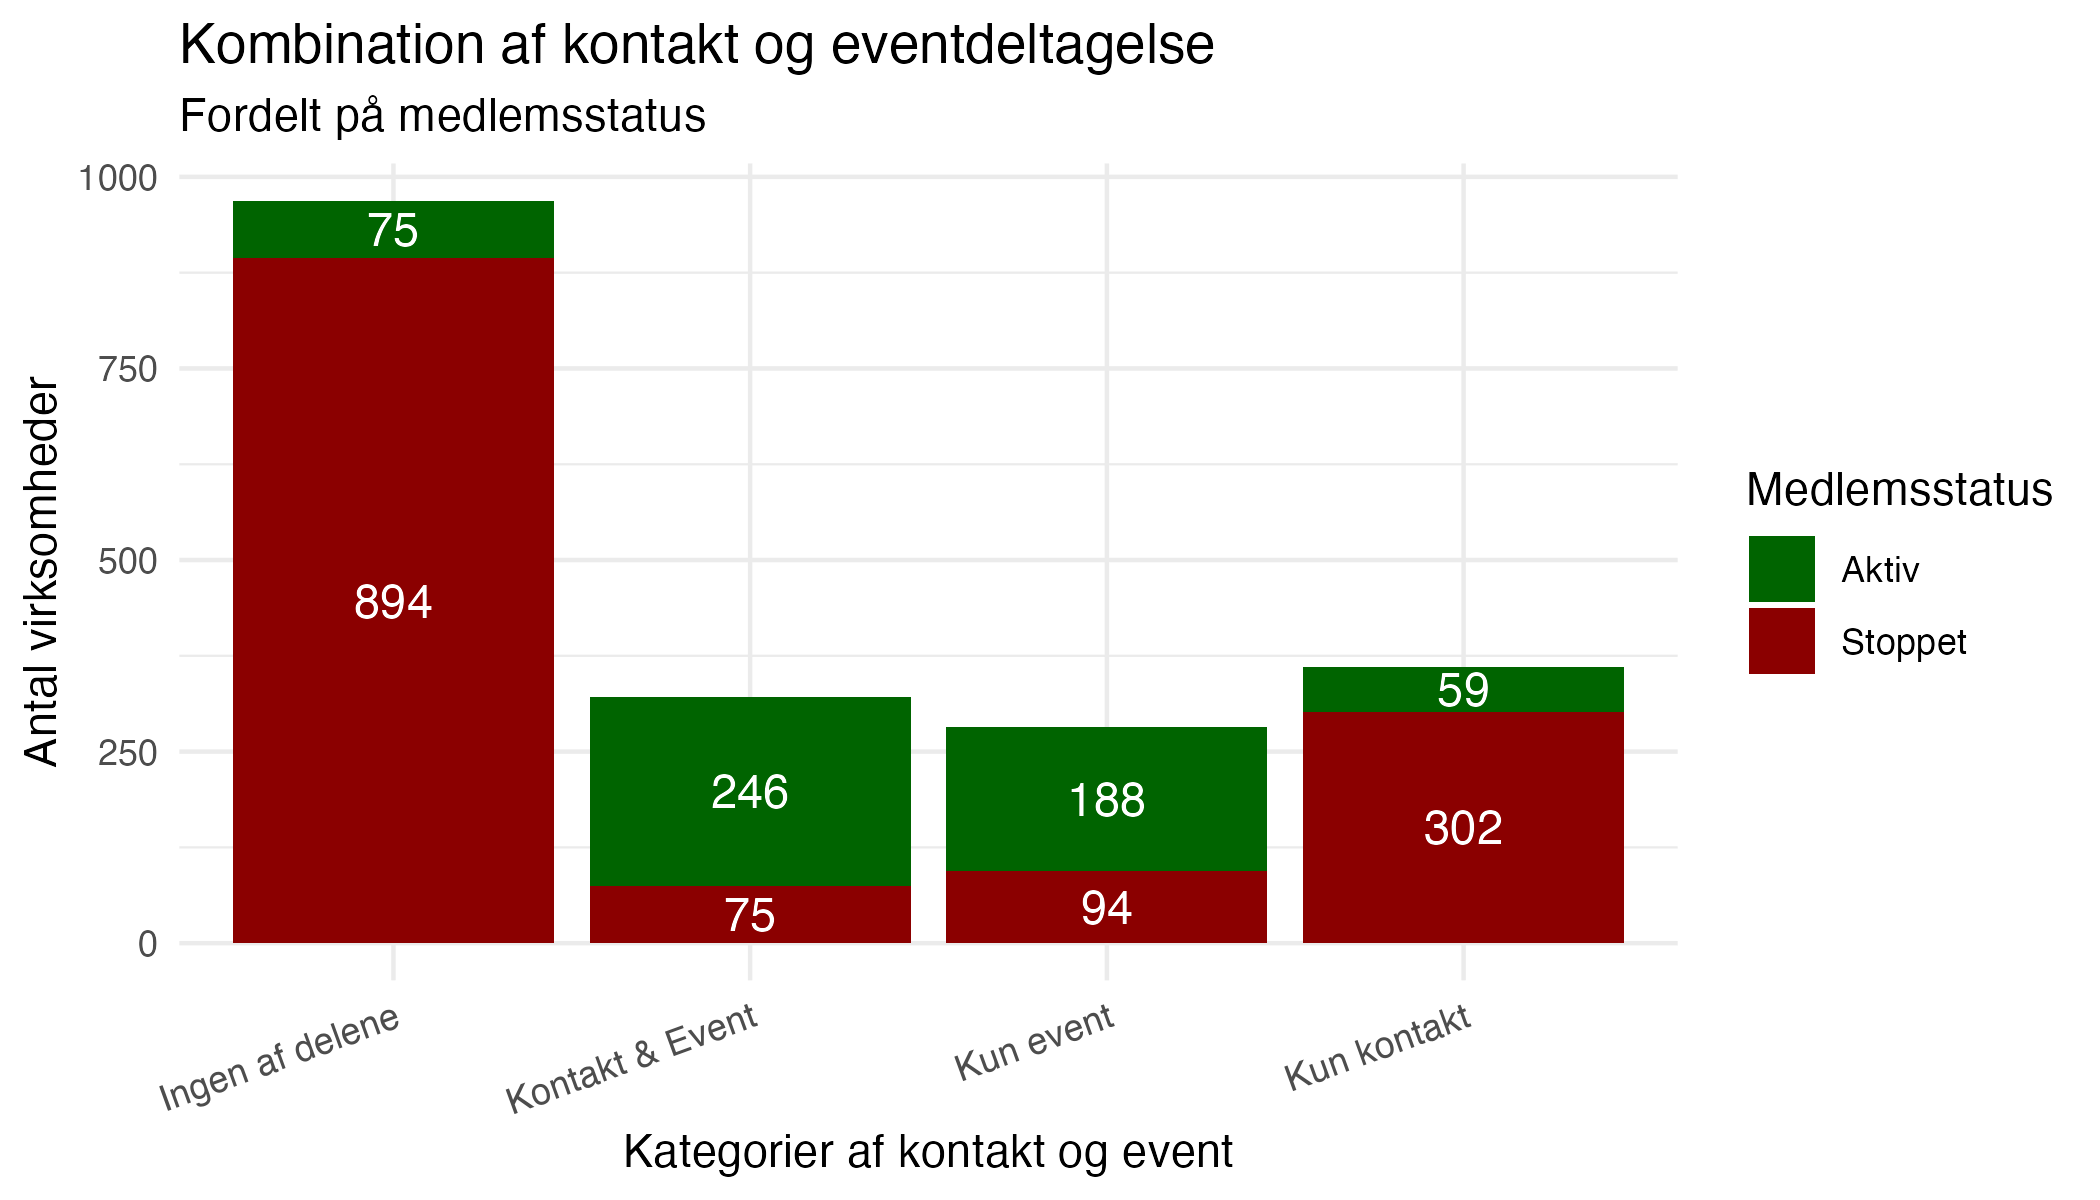
\includegraphics[width=0.8\textwidth,height=\textheight]{images/EDA_3_kombination_kontakt_event.png}

}

\caption{Fravær af begge faktorer er tæt forbundet med udmeldelse, mens
dobbelt engagement viser stærk fastholdelse.}

\end{figure}%

Virksomheder med begrænset kontakt til organisationen, lav deltagelse i
arrangementer og uden dokumenteret interaktion har generelt en markant
højere risiko for at opsige deres medlemskab. Dette underbygges af
figuren nedenfor, der viser de fem postnumre med den højeste
gennemsnitlige churn-risiko. Her ses, at geografiske områder med lav
tilknytning til det centrale område (8800 Viborg) udviser særlig høj
churn-sandsynlighed.

\begin{figure}[H]

{\centering \includegraphics[width=0.8\textwidth,height=\textheight]{images/6_postnummer_højeste_churn.png}

}

\caption{Geografisk afstand fra Viborgs centrum ser ud til at spille en
rolle i udmeldelsestendens. 9620 Aalestrup, 7800 Skive, 7850 Stoholm,
7470 Karup, 8831 Løgstrup}

\end{figure}%

Også på brancheniveau er der tydelige forskelle. Nogle brancher er
kendetegnet ved begrænset interaktion med organisationen og har derfor
en højere sandsynlighed for medlemsophør. Figuren herunder visualiserer
de fem brancher med den højeste gennemsnitlige churn-risiko, hvilket
bekræfter tendensen.

\begin{figure}[H]

{\centering \includegraphics[width=0.8\textwidth,height=\textheight]{images/5_brancher_højeste_churn.png}

}

\caption{Brancher med lav netværksværdi og specialiserede ydelser
udviser generelt højere risiko for medlemsophør.}

\end{figure}%

Omvendt findes der brancher, hvor medlemmerne i langt højere grad
fastholdes. Disse brancher har ofte en mere stabil tilknytning og
deltager aktivt i organisationens tilbud. Den følgende visualisering
viser de fem brancher, hvor medlemmerne i størst omfang forbliver
tilknyttet -- hvilket indikerer, at der her eksisterer en stærkere
relation og et større udbytte af medlemskabet.

\begin{figure}[H]

{\centering 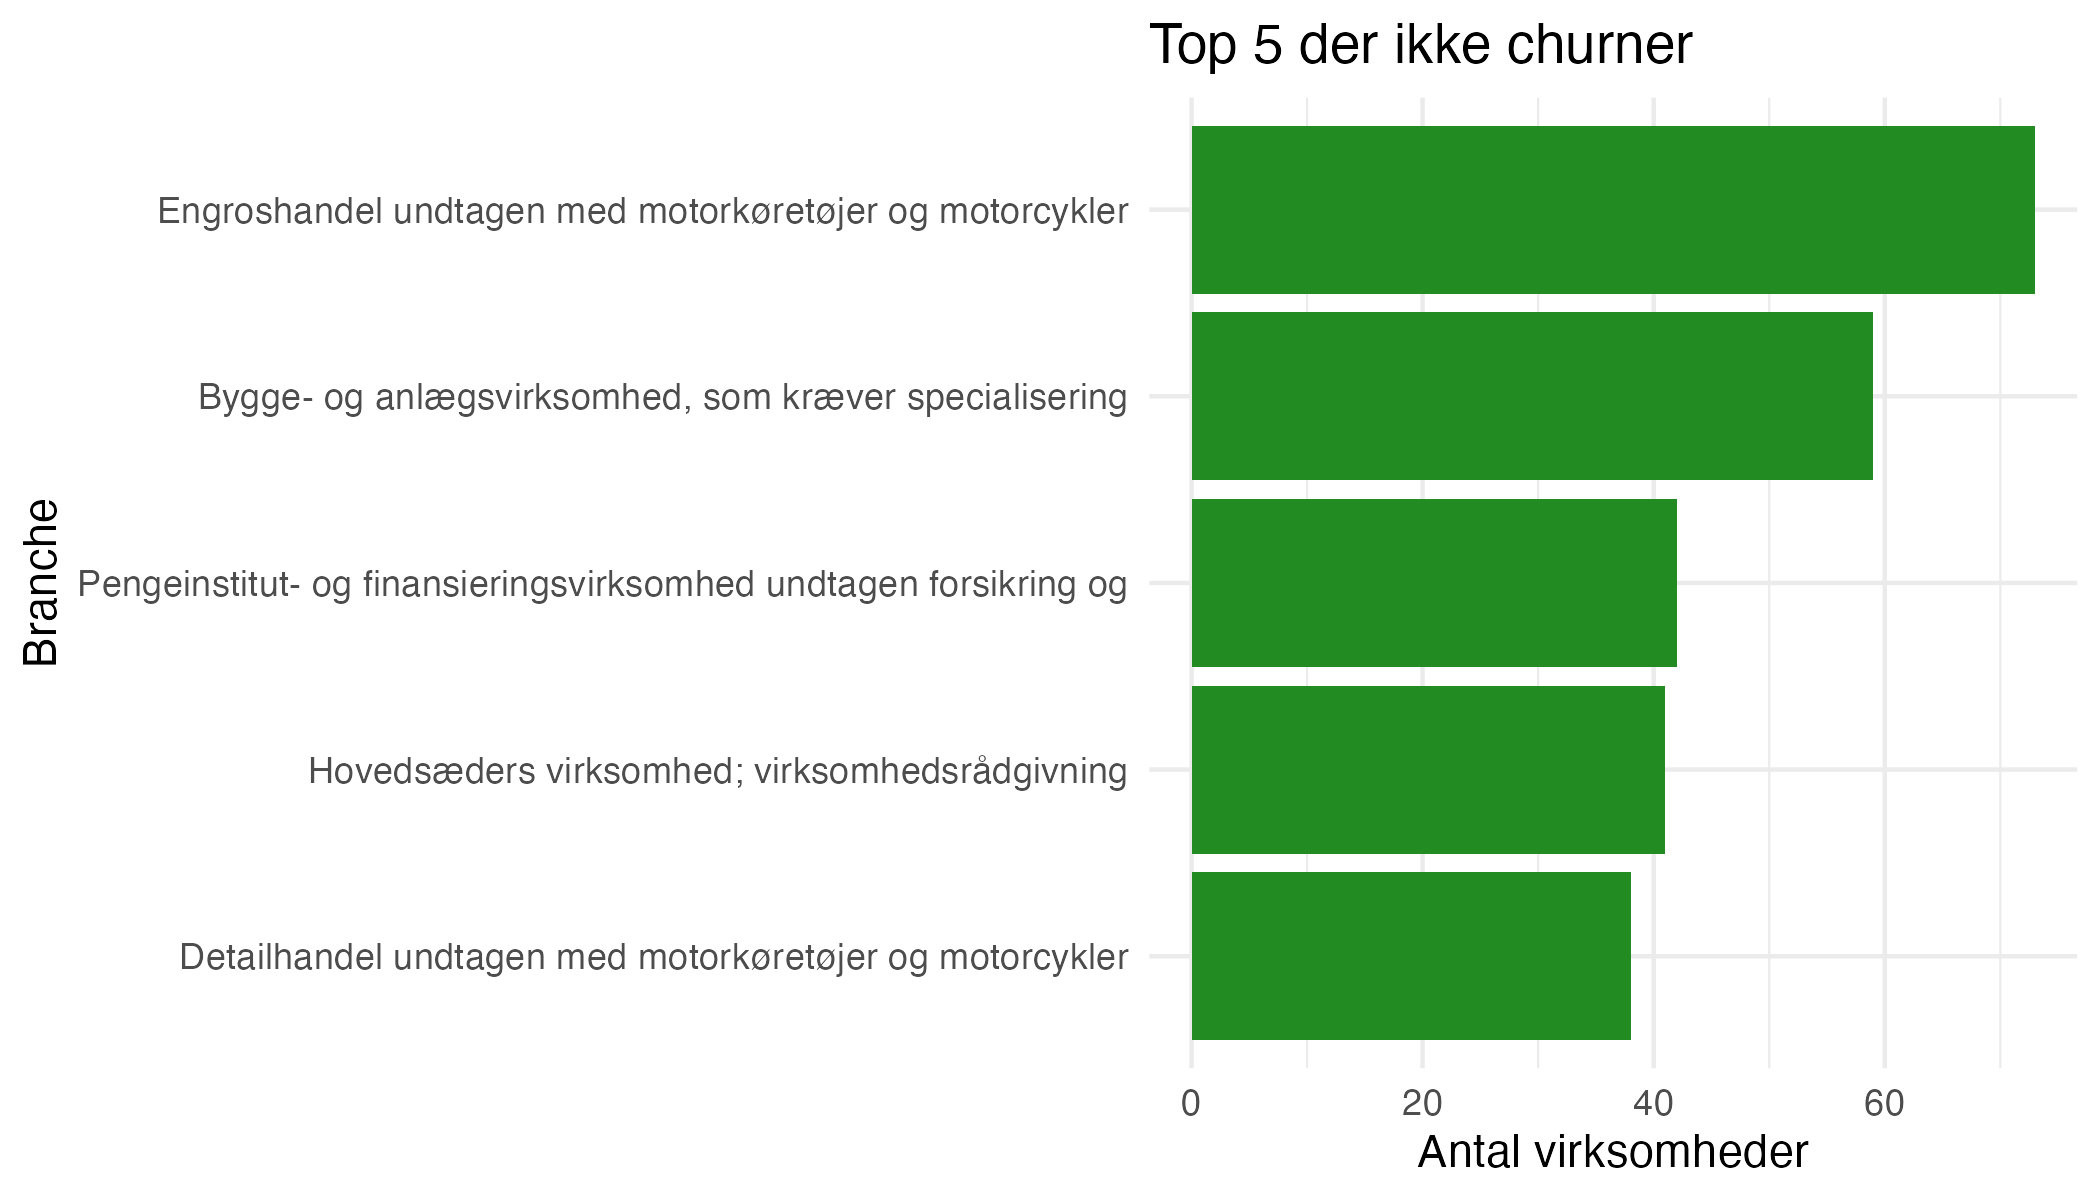
\includegraphics[width=0.8\textwidth,height=\textheight]{images/7_top5_der_ikke_churner.png}

}

\caption{Branchenes høje fastholdelse kan skyldes stærkere relationer og
oplevet værdi af netværket.}

\end{figure}%

I de fem brancher hvor churnrisikoen er lille, er antallet af
virksomheder højt. Dette kunne understøtte teorien om at netværksværdi
har høj prioritet, blandt dem der er medlemmer af Business Viborg.

\subsection{Feature engineering}\label{feature-engineering}

På baggrund af ovenstående mønstre blev der konstrueret nye forklarende
variabler for at styrke modellernes prædiktioner. De mest centrale
inkluderer:

\begin{verbatim}
- medlem_antal_år: længden af medlemskab målt i år
- har_haft_kontakt: binær indikator for, om der har været nogen form for kontakt
- deltaget_i_event: binær indikator for eventdeltagelse
\end{verbatim}

Disse variabler blev udledt på baggrund af domæneviden og eksplorativ
analyse, og bidrog væsentligt til forbedret modelperformance.

\subsection{Modelperformance}\label{modelperformance}

Seks machine learning modeller blev afprøvet: Support Vector Machine
(SVM), XGBoost, Random Forest, logistisk regression, K-nearest Neighbors
(KNN) og Naive Bayes.

\begin{figure}[H]

{\centering 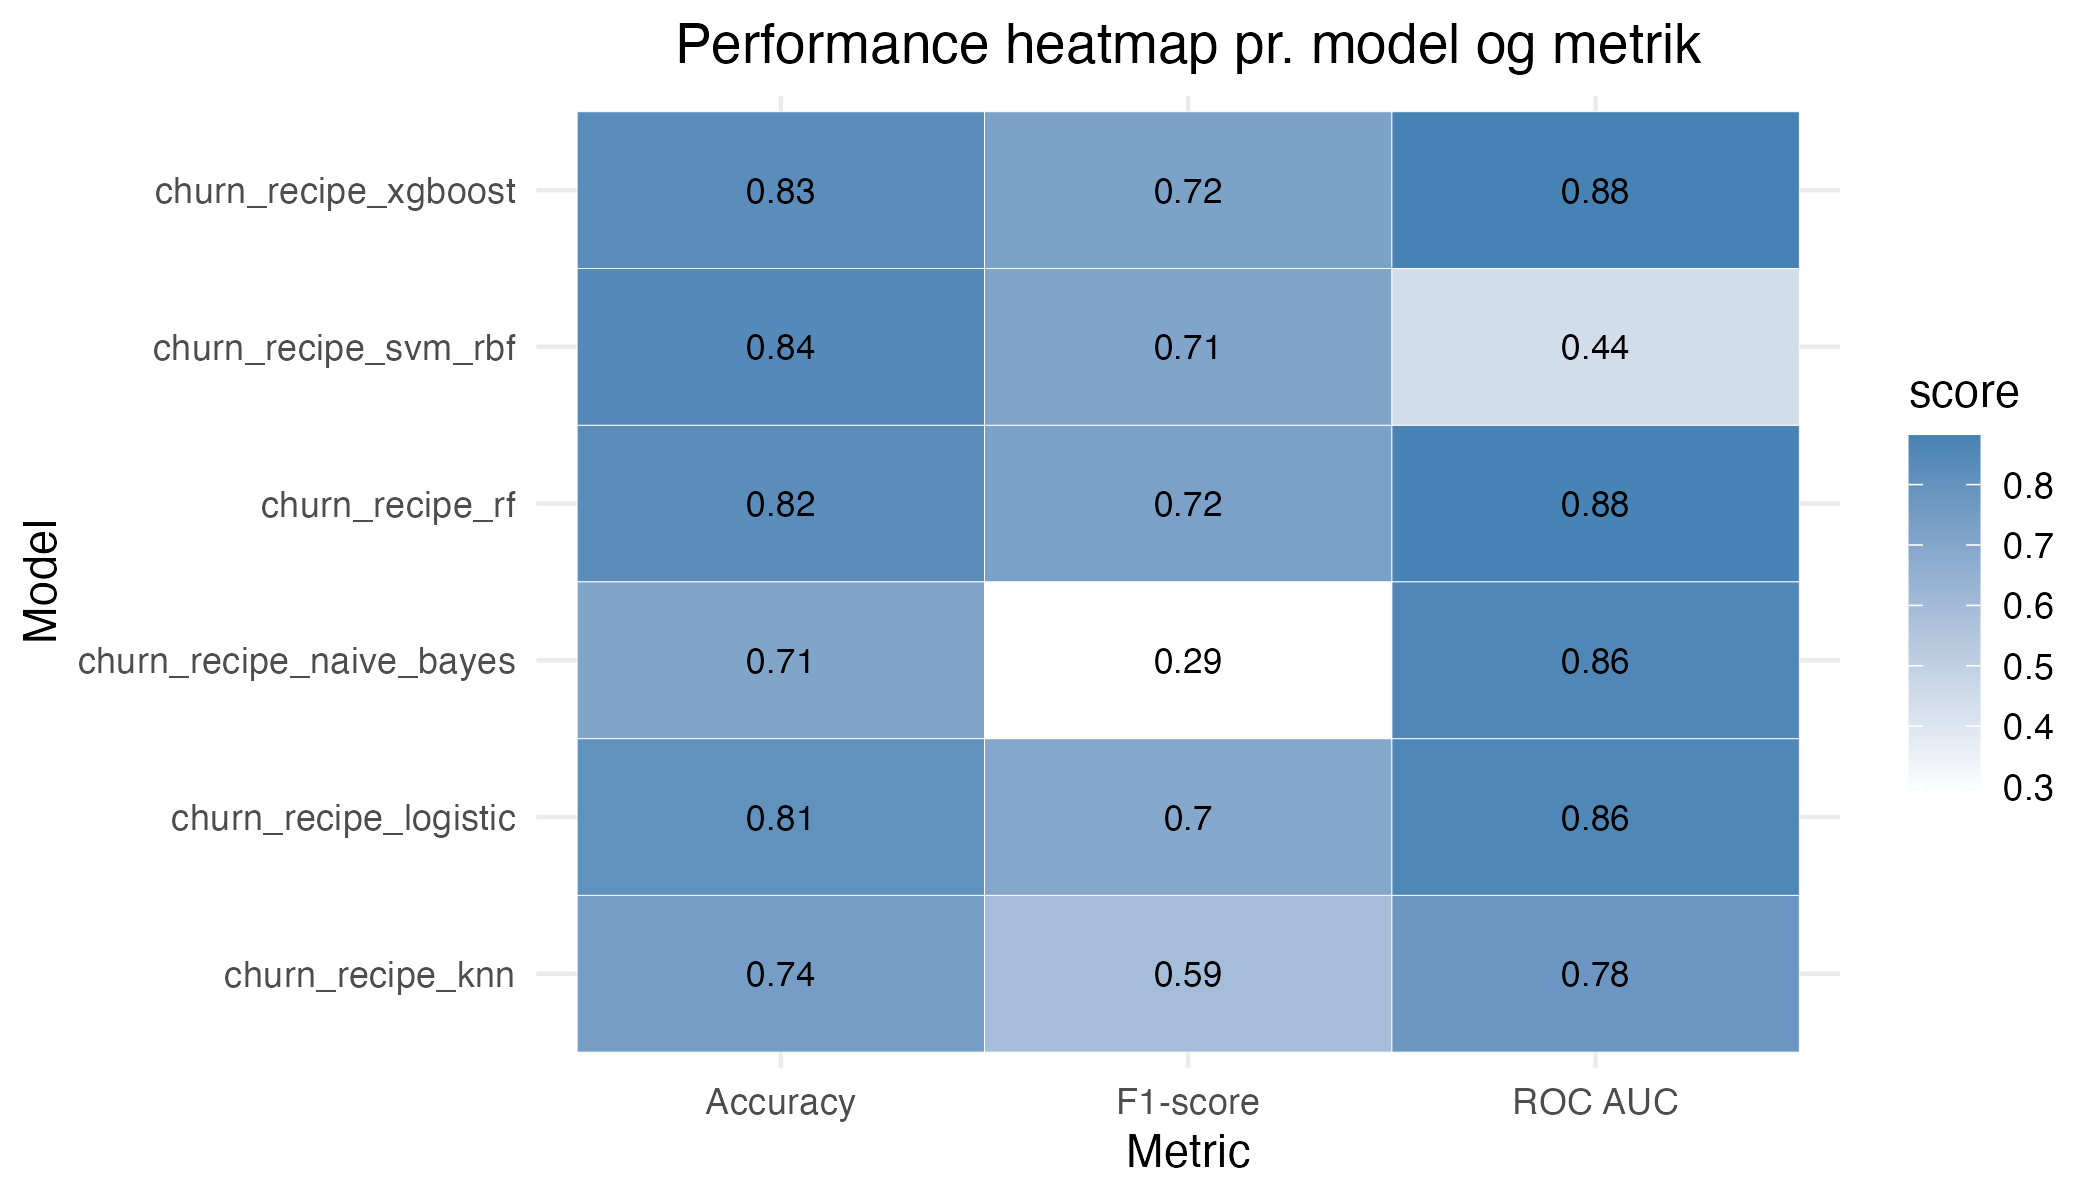
\includegraphics[width=0.8\textwidth,height=\textheight]{images/3_heatmap_pr_model.png}

}

\caption{Farveintensitet viser performance -- mørkere felter angiver
højere score. Random Forest og XGBoost scorer generelt højt, mens Naive
Bayes udviser lav F1-score.}

\end{figure}%

På trods af XGBoost gode resultater blev Random Forest valgt som
slutmodel. Dette skyldes modellens kombination af prædiktiv styrke og
modelgennemsigtighed, hvilket gør den mere anvendelig i en praktisk
kontekst. XGBoost blev fravalgt grundet behovet for yderligere
parameteroptimering, som ikke var formålstjenligt inden for projektets
rammer. Vi valgte den mest simple af de to modeller, da deres metrikker
lå meget tæt.

\begin{figure}[H]

{\centering 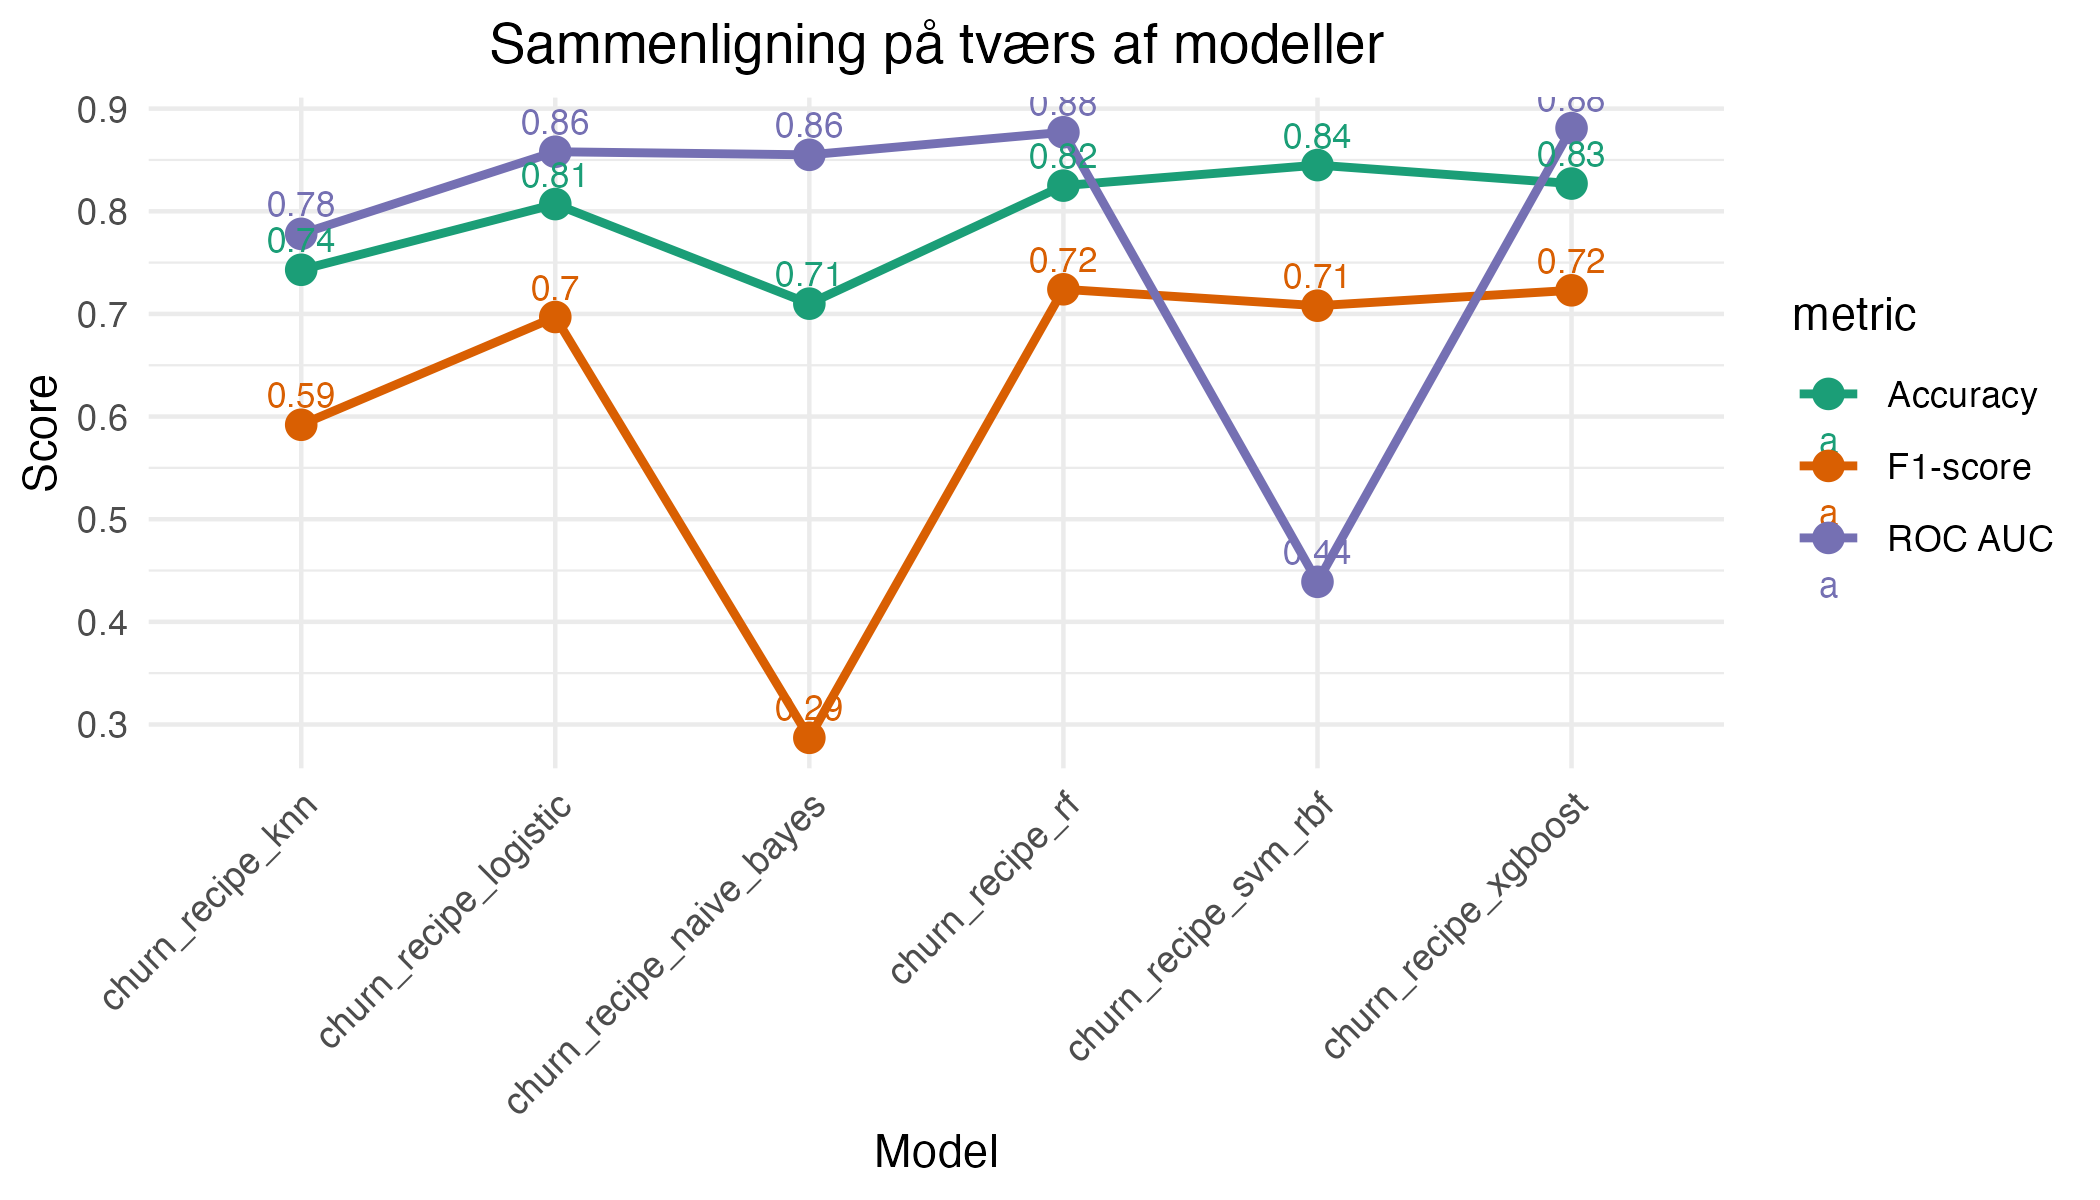
\includegraphics[width=0.8\textwidth,height=\textheight]{images/2_linje_plot.png}

}

\caption{Lineplot over modelperformance. Random Forest og XGBoost opnår
høj score på alle tre metrikker, hvilket underbygger deres styrke som
robuste og præcise modeller.}

\end{figure}%

\subsection{Perspektiv: Modellering af churn over
tid}\label{perspektiv-modellering-af-churn-over-tid}

Da vores datasæt ikke indeholdt tidsstempler for, hvornår virksomheder
præcist meldte sig ud, har vi arbejdet med churn som en binær
klassifikation. Hvis disse oplysninger forelå, ville det være oplagt at
anvende time-to-event-modeller som fx Cox proportional hazards-model.
Disse modeller gør det muligt at estimere, ikke blot om churn
indtræffer, men også hvornår -- hvilket kan styrke den opsøgende indsats
og skabe bedre timing i medlemspleje. Det vil samtidig muliggøre en
dynamisk forståelse af churn-risiko over tid og dermed forbedre
prioriteringen af indsatser.

\subsection{Variable importance og
indsigt}\label{variable-importance-og-indsigt}

Ved hjælp af vip()-pakken blev de mest betydningsfulde variable i Random
Forest-modellen identificeret. De fem vigtigste prædiktorer var:

\begin{itemize}
\tightlist
\item
  deltaget\_i\_event\_Ja
\item
  deltaget\_i\_event\_Nej
\item
  MeetinLenght
\item
  Employees
\item
  medlem\_antal\_år
\end{itemize}

Disse variable udgør tilsammen et stærkt grundlag for at forstå
churn-mekanismer i Business Viborgs medlemsbase og bekræfter den
eksplorative analyses fund.

\begin{figure}[H]

{\centering 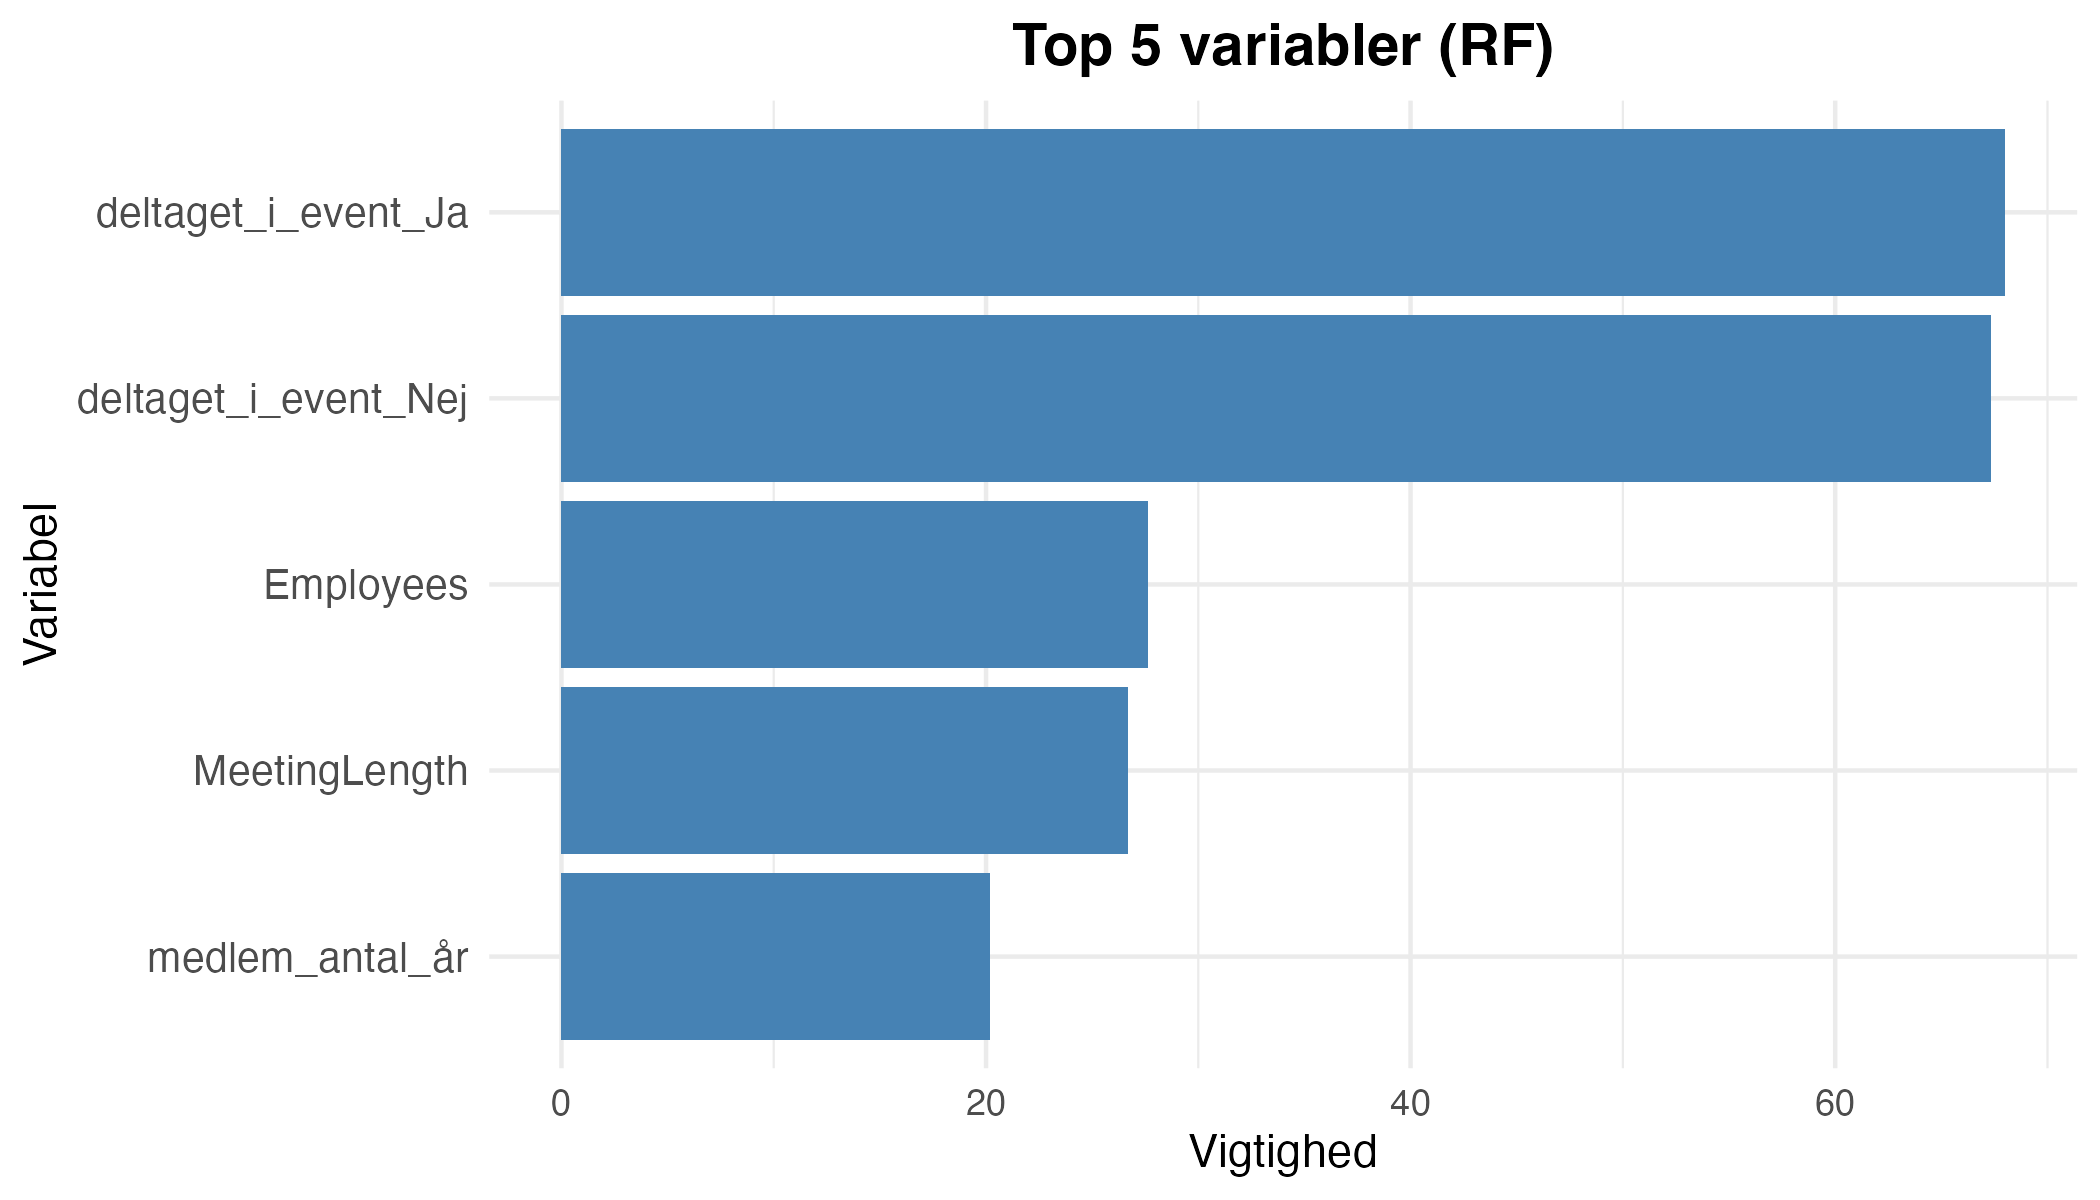
\includegraphics[width=0.8\textwidth,height=\textheight]{images/8_top_5_variabler_rf.png}

}

\caption{Eventdeltagelse, mødelængde, antal ansatte og medlem\_antal\_år
er blandt de mest betydningsfulde prædiktorer for churn.}

\end{figure}%

\subsection{Fordeling af churn-risiko}\label{fordeling-af-churn-risiko}

For at operationalisere modellen i medlemsarbejdet er alle aktive
virksomheder blevet klassificeret i fire risikokategorier baseret på
deres sandsynlighed for churn. Som det fremgår af figuren nedenfor, har
hovedparten af medlemsbasen en lav eller minimal risiko for udmeldelse,
mens en mindre andel er vurderet til at være i moderat eller høj risiko.
Denne fordeling giver medlemskonsulenterne et konkret udgangspunkt for
at prioritere deres indsats og målrette dialogen mod virksomheder i
risikozonen.

\begin{figure}[H]

{\centering 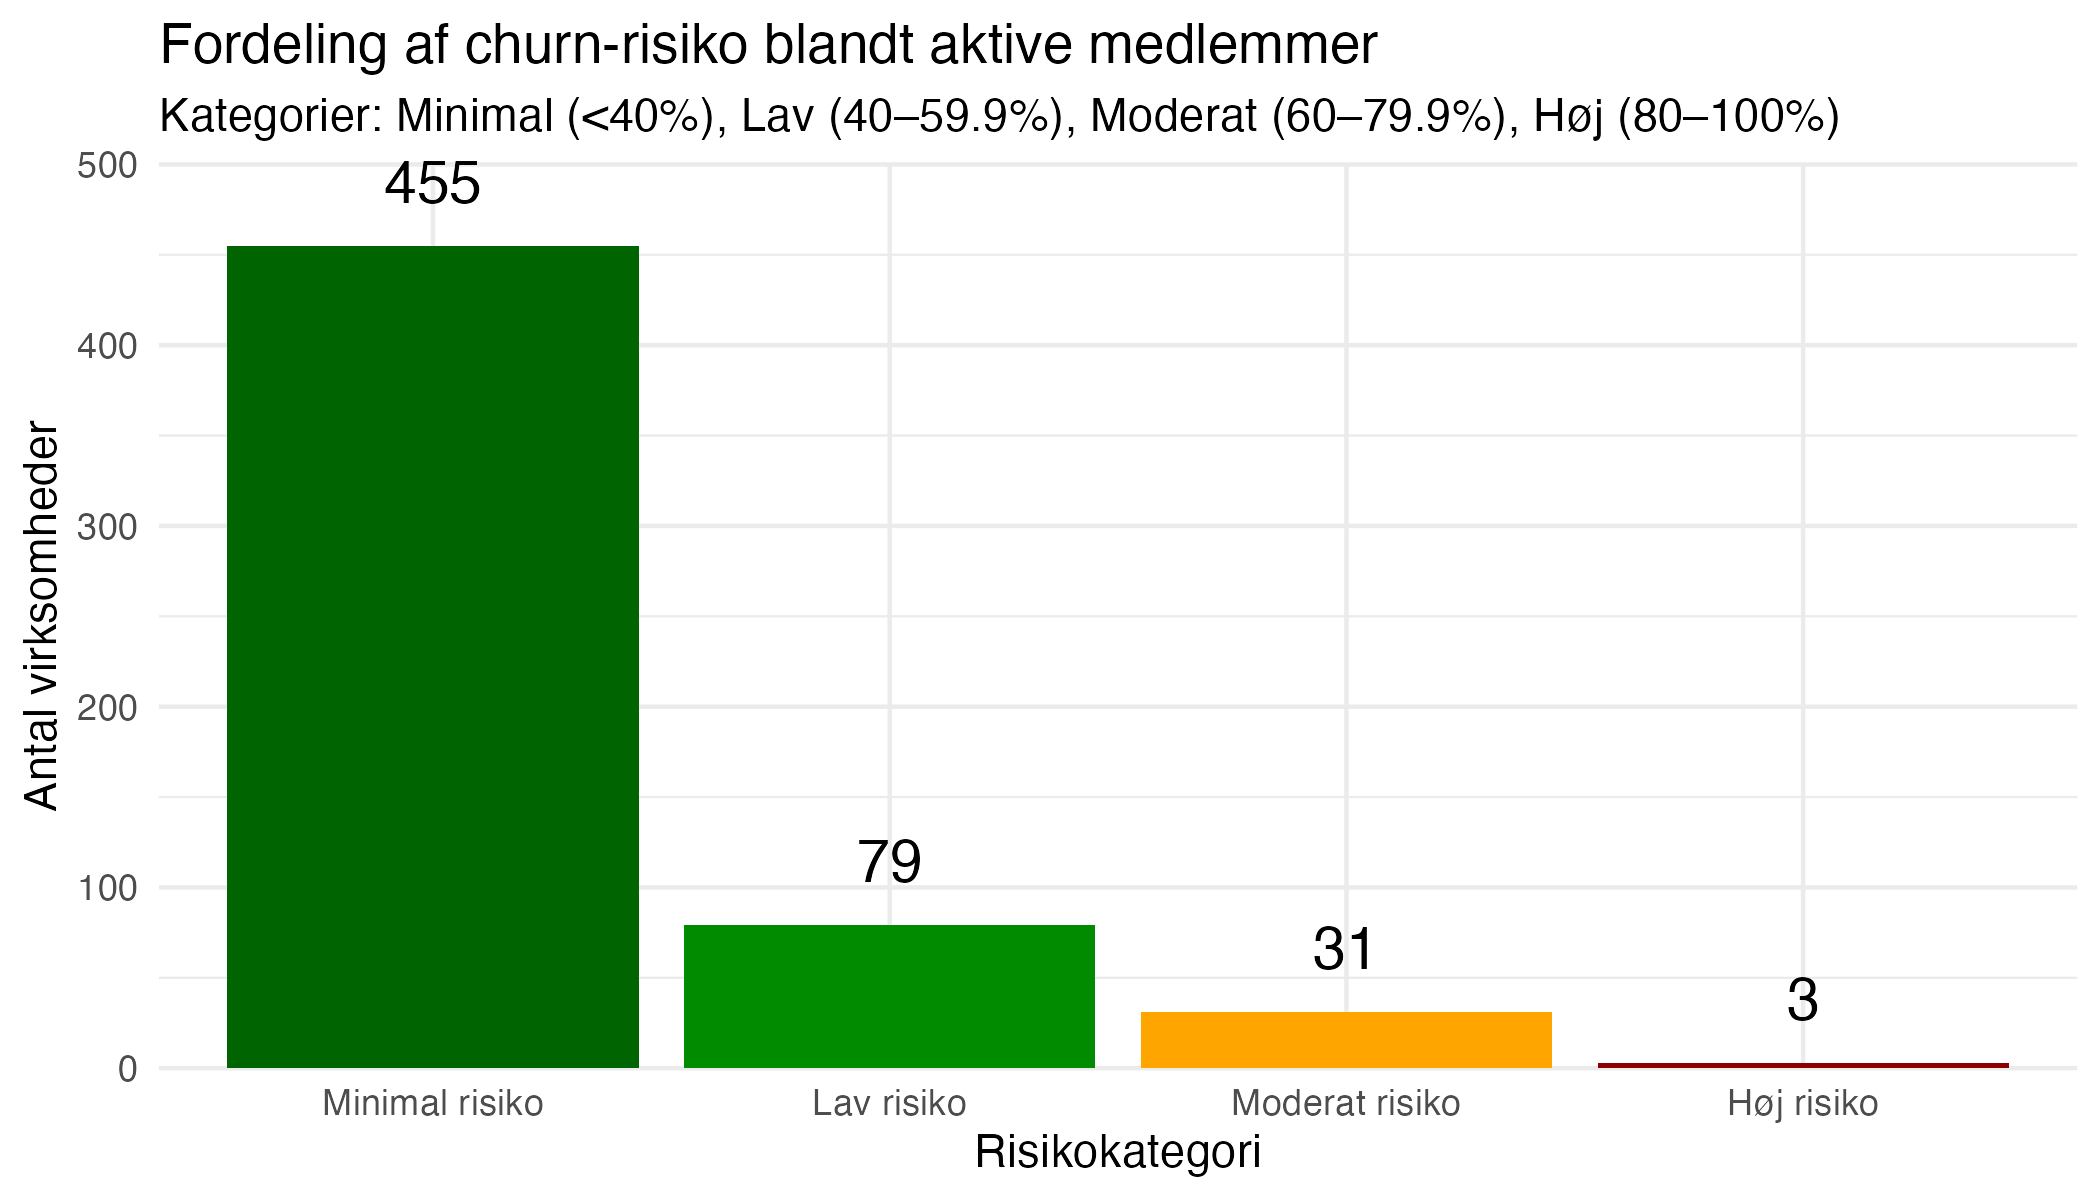
\includegraphics[width=0.8\textwidth,height=\textheight]{images/9_churn_risikokategorier_aktive.png}

}

\caption{Fordeling af churn-risiko blandt aktive medlemmer baseret på
modelprediktioner. Kategorierne ``høj risiko'' og ``moderat risiko''
rummer 38 virksomheder. De udgør et vigtigt proaktivt fokuspunkt.}

\end{figure}%

\section{Anvendelse af dashboard i
medlemsarbejdet}\label{anvendelse-af-dashboard-i-medlemsarbejdet}

Som led i samarbejdet med Business Viborg har vi udviklet et interaktivt
dashboard, der omsætter churn-modellens output til konkret
medlemsindsigt. Dashboardet er målrettet konsulenterne og ledelsen og
gør det muligt at identificere medlemmer med høj risiko for at opsige
deres medlemskab. Visualiseringen er designet til at passe ind i
konsulenternes og ledelsens arbejdsgange og skabe et klart
beslutningsgrundlag i hverdagen.

\textbf{Adgangsoplysninger:}

\begin{itemize}
\tightlist
\item
  \textbf{Link:}
  \url{https://maria-cristiana-maxim.shinyapps.io/churnapp/}\\
\item
  \textbf{Brugernavn:} \texttt{admin@businessviborg.com}\\
\item
  \textbf{Adgangskode:} \texttt{Test1234}
\end{itemize}

\begin{quote}
\emph{Dashboardet er en prototype og bør anvendes til
demonstrationsformål. Ved implementering i praksis anbefales det at
justere adgangskontrol, datasikkerhed og systemintegration.}
\end{quote}

\begin{figure}[H]

{\centering 
\includegraphics[width=0.1\textwidth,height=\textheight]{images/churn_dashboard_qr.png}

}

\caption{QR-kode til churn-dashboard}

\end{figure}%

\section{Juridiske og etiske
overvejelser}\label{juridiske-og-etiske-overvejelser}

\subsection{Juridiske og etiske forhold i churn-projektet for Business
Viborg}\label{juridiske-og-etiske-forhold-i-churn-projektet-for-business-viborg}

I forbindelse med udviklingen af en datadrevet løsning til forudsigelse
af medlems-churn hos Business Viborg er det essentielt, at både
juridiske og etiske hensyn bliver nøje overvejet og integreret i hele
udviklingsprocessen. Den teknologiske og analytiske dimension af
projektet må ikke stå alene, men skal suppleres af en bevidsthed om
datasikkerhed, individets rettigheder og ansvarlig brug af data. Da
løsningen tager udgangspunkt i oplysninger om organisationens medlemmer,
der potentielt kan knyttes til identificerbare personer, er
databehandlingen omfattet af EU's Databeskyttelsesforordning (GDPR).
Dette gælder, uanset om data fremstår pseudonymiserede for os som
analytikere, da Business Viborg internt kan koble data til konkrete
virksomheder eller kontaktpersoner. Formålet med dette afsnit er derfor
at belyse de centrale juridiske forpligtelser samt de etiske
retningslinjer, som Business Viborg bør overholde i forbindelse med
udviklingen og implementeringen af churn-modellen.

\subsection{Behandlingsgrundlag}\label{behandlingsgrundlag}

Et fundamentalt krav i GDPR er, at al behandling af personoplysninger
skal have et lovligt behandlingsgrundlag. Business Viborgs
databehandling relaterer sig til almindelige personoplysninger såsom
virksomhedsnavne, kontaktoplysninger, mødedeltagelse og
interaktionshistorik. Det er derfor nødvendigt at vurdere, hvilket
hjemmelsgrundlag der gør det lovligt at anvende disse data i en
churn-model. Ifølge artikel 6 i GDPR kan behandlingen enten baseres på
samtykke fra medlemmerne (art. 6, stk. 1, litra a) eller på
organisationens legitime interesser (art. 6, stk. 1, litra f). I denne
kontekst vurderes det, at Business Viborg primært bør benytte den
legitime interesse som behandlingsgrundlag, da organisationens formål --
at forbedre medlemsservice, understøtte fastholdelse og sikre et
bæredygtigt erhvervsfællesskab -- er både sagligt, proportionalt og
foreneligt med medlemmernes forventninger. Det er dog vigtigt at
bemærke, at hvis data senere anvendes til andre formål, f.eks. målrettet
markedsføring eller automatiseret profilering, kan det være nødvendigt
at genoverveje behandlingsgrundlaget, herunder at indhente eksplicit
samtykke.

\subsection{Personoplysninger og
dataminimering}\label{personoplysninger-og-dataminimering}

Analyserne tager udgangspunkt i almindelige personoplysninger, som ikke
i sig selv er følsomme, men som i kombination med andre oplysninger
stadig udgør personoplysninger i GDPR-forstand. Eksempler kan være data
om deltagelse i arrangementer, mødeaktivitet eller medlemskabets
varighed. For at overholde principperne om dataminimering og
formålsbegrænsning (jf. GDPR art. 5), skal Business Viborg sikre, at der
kun behandles data, som er nødvendige og relevante i forhold til det
definerede formål -- nemlig at kunne identificere virksomheder i risiko
for udmeldelse. Alle unødvendige oplysninger bør fjernes eller
anonymiseres, og det samlede datasæt skal reduceres til det minimum, der
kræves for at modellere churn med høj præcision. Derudover skal der være
dokumentation for, hvordan og hvorfor de valgte variabler indgår i
modellen. Denne dokumentation skal kunne anvendes til intern kontrol og
overfor Datatilsynet, hvis der føres tilsyn.

\subsection{Oplysningspligt og
transparens}\label{oplysningspligt-og-transparens}

Business Viborg har i henhold til GDPR artikel 13 og 14 en klar
oplysningspligt over for de registrerede medlemmer. Det betyder, at
medlemmerne skal informeres om, at deres data indgår i analyser, hvad
formålet med analysen er, hvilke rettigheder de har, og hvordan de kan
kontakte organisationen for spørgsmål eller indsigelser. Oplysningen bør
være let tilgængelig og formuleret i et sprog, der er forståeligt for
ikke-specialister. Ideelt set bør informationen formidles både via
organisationens privatlivspolitik og i forbindelse med
medlemskommunikation -- f.eks. i velkomstmateriale eller nyhedsbreve.
Transparens er i denne sammenhæng ikke blot et juridisk krav, men også
et middel til at styrke medlemmernes tillid til Business Viborgs
databrug.

\subsection{Pseudonymisering og
identifikationsrisici}\label{pseudonymisering-og-identifikationsrisici}

Selvom datasættet, som analysen baseres på, er pseudonymiseret for
dataanalytikerne, betyder det ikke, at oplysningerne er anonyme i
GDPR-forstand. Business Viborgs medarbejdere har adgang til
nøgleoplysninger såsom medlemsnummer, virksomhedsnavn eller
kontaktpersoner, som gør det muligt at identificere de registrerede.
Dette understreger, at databehandlingen fortsat er omfattet af alle
GDPR-krav. Der skal derfor træffes passende forholdsregler for at sikre,
at oplysningerne ikke anvendes til andre formål uden nyt
behandlingsgrundlag og ikke utilsigtet afslører følsom information om
specifikke virksomheder. Datasikkerhed og organisatorisk ansvar Business
Viborg er som dataansvarlig forpligtet til at beskytte personoplysninger
mod uautoriseret adgang, tab, ændring eller misbrug. I henhold til
artikel 24 og 32 i GDPR skal organisationen iværksætte både tekniske og
organisatoriske sikkerhedsforanstaltninger. Det inkluderer brug af
adgangsstyring, kryptering, logning af datatilgange, opdaterede
sikkerhedspolitikker og uddannelse af personale i datasikkerhed.
Derudover skal der foreligge databehandleraftaler, hvis eksterne
samarbejdspartnere inddrages i projektet. Manglende sikkerhed kan ikke
alene få juridiske konsekvenser, men også underminere den tillid, som
projektet skal baseres på.

\subsection{Etiske overvejelser og ansvarlig
dataanvendelse}\label{etiske-overvejelser-og-ansvarlig-dataanvendelse}

Udover den juridiske ramme bør Business Viborg også forholde sig aktivt
til dataetik og samfundsansvar. Ifølge anbefalinger fra bl.a. Dataetisk
Råd handler ansvarlig dataanvendelse om at sætte mennesket i centrum,
sikre gennemsigtighed og undgå skævvridning eller diskrimination.
Anvendelsen af en churn-model må ikke resultere i, at bestemte
virksomheder eller grupper automatisk vurderes som mindre værdifulde
baseret på statistiske mønstre, som ikke er sagligt begrundede. Der skal
derfor tages højde for fairness og risikoen for bias -- både i
datasættets sammensætning og i de variable, der anvendes i modellen.
Transparens er også afgørende her: medarbejdere skal kunne forstå og
forklare modellens logik og resultater. En ``black box''-model, som ikke
kan forklares, kan føre til uforståelige eller urimelige beslutninger,
hvilket ikke er foreneligt med en ansvarlig og tillidsvækkende
medlemsorganisation. Ledelsen i Business Viborg har desuden et særligt
ansvar for at sikre, at modellen anvendes i overensstemmelse med
organisationens værdier. Det anbefales derfor, at der formuleres en
dataetik-politik, som dækker ansvar, kontrol og kommunikation i relation
til anvendelsen af churn-modellen. Politikken bør revideres løbende i
takt med, at modellen og databrug udvikles.

\subsection{Må Business Viborg beholde data på udmeldte
medlemmer}\label{muxe5-business-viborg-beholde-data-puxe5-udmeldte-medlemmer}

Ifølge GDPR artikel 5, stk. 1, litra e, må personoplysninger ikke
opbevares længere end nødvendigt til det formål, de er indsamlet til.
Når et medlem melder sig ud, er det normale formål -- f.eks.
kommunikation, arrangementer eller medlemsservice -- ikke længere
aktuelt.

Men der kan være lovlige grunde til at opbevare dem i en periode
Business Viborg må godt gemme data i en vis periode efter udmeldelse,
hvis de har et sagligt og dokumenteret formål, f.eks.:

\begin{itemize}
\tightlist
\item
  Bogføring og regnskab -- fx fakturaer, betalinger osv. må gerne
  opbevares i op til 5 år (jf. Bogføringsloven).
\item
  Statistisk analyse -- men kun hvis data anonymiseres eller
  pseudonymiseres, så det ikke længere er muligt at identificere
  personen uden ekstra oplysninger.
\item
  Retligt forsvar -- hvis der er risiko for tvister eller krav, kan man
  argumentere for at opbevare data i en periode, typisk op til
  forældelsesfristen (som ofte er 3 år i civile sager).
\end{itemize}

De må ikke fortsætte med at bruge tidligere medlemmers data til
markedsføring og ikke opbevare data ``bare for en sikkerheds skyld''
uden formål og dokumentation.

CVR-numre tilknyttet enkeltmandsvirksomheder betragtes som
personoplysninger, da de kan føres direkte tilbage til en fysisk person
-- virksomhedens ejer. Selvom disse oplysninger identificerer en person,
klassificeres de ikke som følsomme oplysninger i henhold til GDPR's
artikel 9, da de ikke afslører forhold som helbred, politisk
overbevisning eller religiøs tilhørsforhold. CVR-oplysninger er desuden
offentligt tilgængelige og indgår derfor under almindelige
personoplysninger, som stadig skal behandles i overensstemmelse med
GDPR's generelle principper.

\subsection{Delonklusion}\label{delonklusion}

Sammenfattende vurderes det, at Business Viborgs churn-projekt kan
gennemføres i overensstemmelse med GDPR og etiske retningslinjer,
forudsat at visse betingelser overholdes. Der skal foreligge et klart og
dokumenteret behandlingsgrundlag, medlemmerne skal informeres tydeligt
og rettidigt, og datasættet skal reduceres til relevante oplysninger i
henhold til formålet. Desuden skal organisationen sikre passende
tekniske og organisatoriske sikkerhedsforanstaltninger og være opmærksom
på, at data fortsat er personhenførbare, selvom de fremstår
pseudonymiserede. Afslutningsvis bør Business Viborg betragte dette
projekt som et skridt mod mere datadrevet medlemsservice -- men også som
en mulighed for at styrke sin rolle som en ansvarlig og gennemsigtig
aktør i det lokale erhvervsliv. Det forudsætter, at juridiske
forpligtelser og dataetiske principper ikke ses som forhindringer, men
som en integreret del af en moderne og tillidsbaseret organisation.

\section{Anbefaling}\label{anbefaling}

På baggrund af analysen anbefales det, at Business Viborg anvender den
udviklede churn-model som et beslutningsunderstøttende værktøj i det
opsøgende medlemsarbejde. Modellen kan identificere virksomheder med høj
risiko for udmeldelse og derved muliggøre en mere målrettet og proaktiv
indsats fra medlemskonsulenterne. Det foreslås, at den udviklede Shiny
app indgår som fast element i konsulenternes arbejdsrutiner og
prioritering af medlemmer.

\begin{itemize}
\item
  Medlemspleje prioriteres over for virksomheder uden kontakt,
  eventdeltagelse eller modtaget hjælp, da disse faktorer er stærkt
  associeret med churn. Særligt events er relevante for at bibeholde
  medlemmerne. De har allerede mange events, men det kunne anbefales at
  lave flere skræddersyede events, så man sænker risikoen for churn på
  samtlige medlemmer.
\item
  Løbende opdatering af modellen sikres ved at integrere churn-værktøjet
  i Business Viborgs CRM eller medlemsdatabase, så nye data automatisk
  indgår i fremtidige analyser.
\item
  Etisk og transparent kommunikation om brugen af data indgår i
  medlemsdialogen for at styrke tilliden og sikre overholdelse af GDPR.
\end{itemize}

\section{Konklusion}\label{konklusion}

Projektet har vist, hvordan Business Viborg med et afgrænset
datagrundlag og begrænsede ressourcer kan anvende machine learning som
et konkret værktøj til medlemsfastholdelse. Gennem analyse af 2.966
medlemsvirksomheder og systematisk afprøvning af seks modeller blev der
udviklet en forklarlig Random Forest-model med stærke prædiktive
egenskaber (F1 = 0,79, AUC = 0,93). Modellen er operationaliseret i et
interaktivt dashboard, som giver medlemskonsulenterne og ledelse et
datadrevet grundlag for at prioritere og målrette deres opsøgende
indsats.

Resultaterne peger entydigt på, at fravær af kontakt, manglende
eventdeltagelse og manglende erhvervshjælp er tæt knyttet til
udmeldelse. Samtidig viser analysen, at en langvarig relation og
relationel dybde -- målt gennem fx mødelængde -- hænger tæt sammen med
fastholdelse. Denne indsigt skaber en direkte kobling mellem data og
daglig praksis i medlemsarbejdet. Den største faktor er deltagelse i
events og der kan med fordel udvikles skræddersyede events, der skaber
værdi og dermed fastholdelse af flere medlemmer.

Modellen er udviklet med udgangspunkt i GDPR og principper om ansvarlig
dataanvendelse. Det understreger, at datadrevne løsninger godt kan gå
hånd i hånd med transparens, etik og tillid. Der er taget højde for både
behandlingsgrundlag, oplysningspligt og identifikationsrisici -- og
løsningen kan derfor fungere som en ansvarlig prototype, der med de
rette tekniske og organisatoriske rammer kan bringes i anvendelse.

Et naturligt næste skridt er at inddrage tidsstempler for udmeldelser.
Det vil gøre det muligt ikke kun at vurdere risikoen for churn, men også
at estimere, hvornår en udmeldelse sandsynligvis vil finde sted. Dermed
får Business Viborg et endnu bedre grundlag for at igangsætte målrettede
og rettidige indsatser over for medlemmer i risiko.

Samlet set besvarer projektet sin problemformulering ved at kombinere
teknisk analyse, brugervenlig formidling og etisk ansvarlighed. Det
peger samtidig frem mod en bredere anvendelse af datadrevne
beslutningsværktøjer i medlemsorganisationer, der ønsker at arbejde
strategisk og relationsbaseret -- uden at give køb på tillid,
menneskelig dømmekraft og lokal forankring.

\newpage

\section{Litteraturliste}\label{litteraturliste}

\textbf{AI}

OpenAI. (2025). ChatGPT (version 4.0). Hentet fra https://chatgpt.com/

\textbf{Bøger}

Wickham, H., Çetinkaya-Rundel, M., \& Grolemund, G. (2023). R for Data
Science (2. udg.). O'Reilly Media. Hentet fra https://r4ds.hadley.nz/

Wickham, H. (2016). ggplot2: Elegant Graphics for Data Analysis (2.
udg.). Springer. Hentet fra https://ggplot2-book.org/

Kuhn, M., \& Silge, J. (2022). Tidy Modeling with R. O'Reilly Media.
Hentet fra https://www.tmwr.org/

\textbf{WWW-dokumenter}

Europa-Parlamentet og Rådet. (2016). Forordning (EU) 2016/679 -- Generel
forordning om databeskyttelse (GDPR). Hentet fra
https://eur-lex.europa.eu/legal-content/DA/TXT/?uri=CELEX\%3A32016R0679

Erhvervsstyrelsen. (2025). Vejledning til bogføringsloven. Hentet fra
https://erhvervsstyrelsen.dk/vejledning-bogfoeringsloven

Dataetisk Råd. (2025). Officielt websted for Dataetisk Råd. Hentet fra
https://dataetiskraad.dk/

\newpage

\section{Bilagsoversigt}\label{bilagsoversigt}

\subsection{Bilag 1--6: Eksplorativ
dataanalyse}\label{bilag-16-eksplorativ-dataanalyse}

Anvendt i forbindelse med udarbejdelse og forståelse af datasættet:

\begin{itemize}
\tightlist
\item
  \textbf{Bilag 1:} Fordeling af medlemmer hos Business Viborg
\end{itemize}

\begin{center}
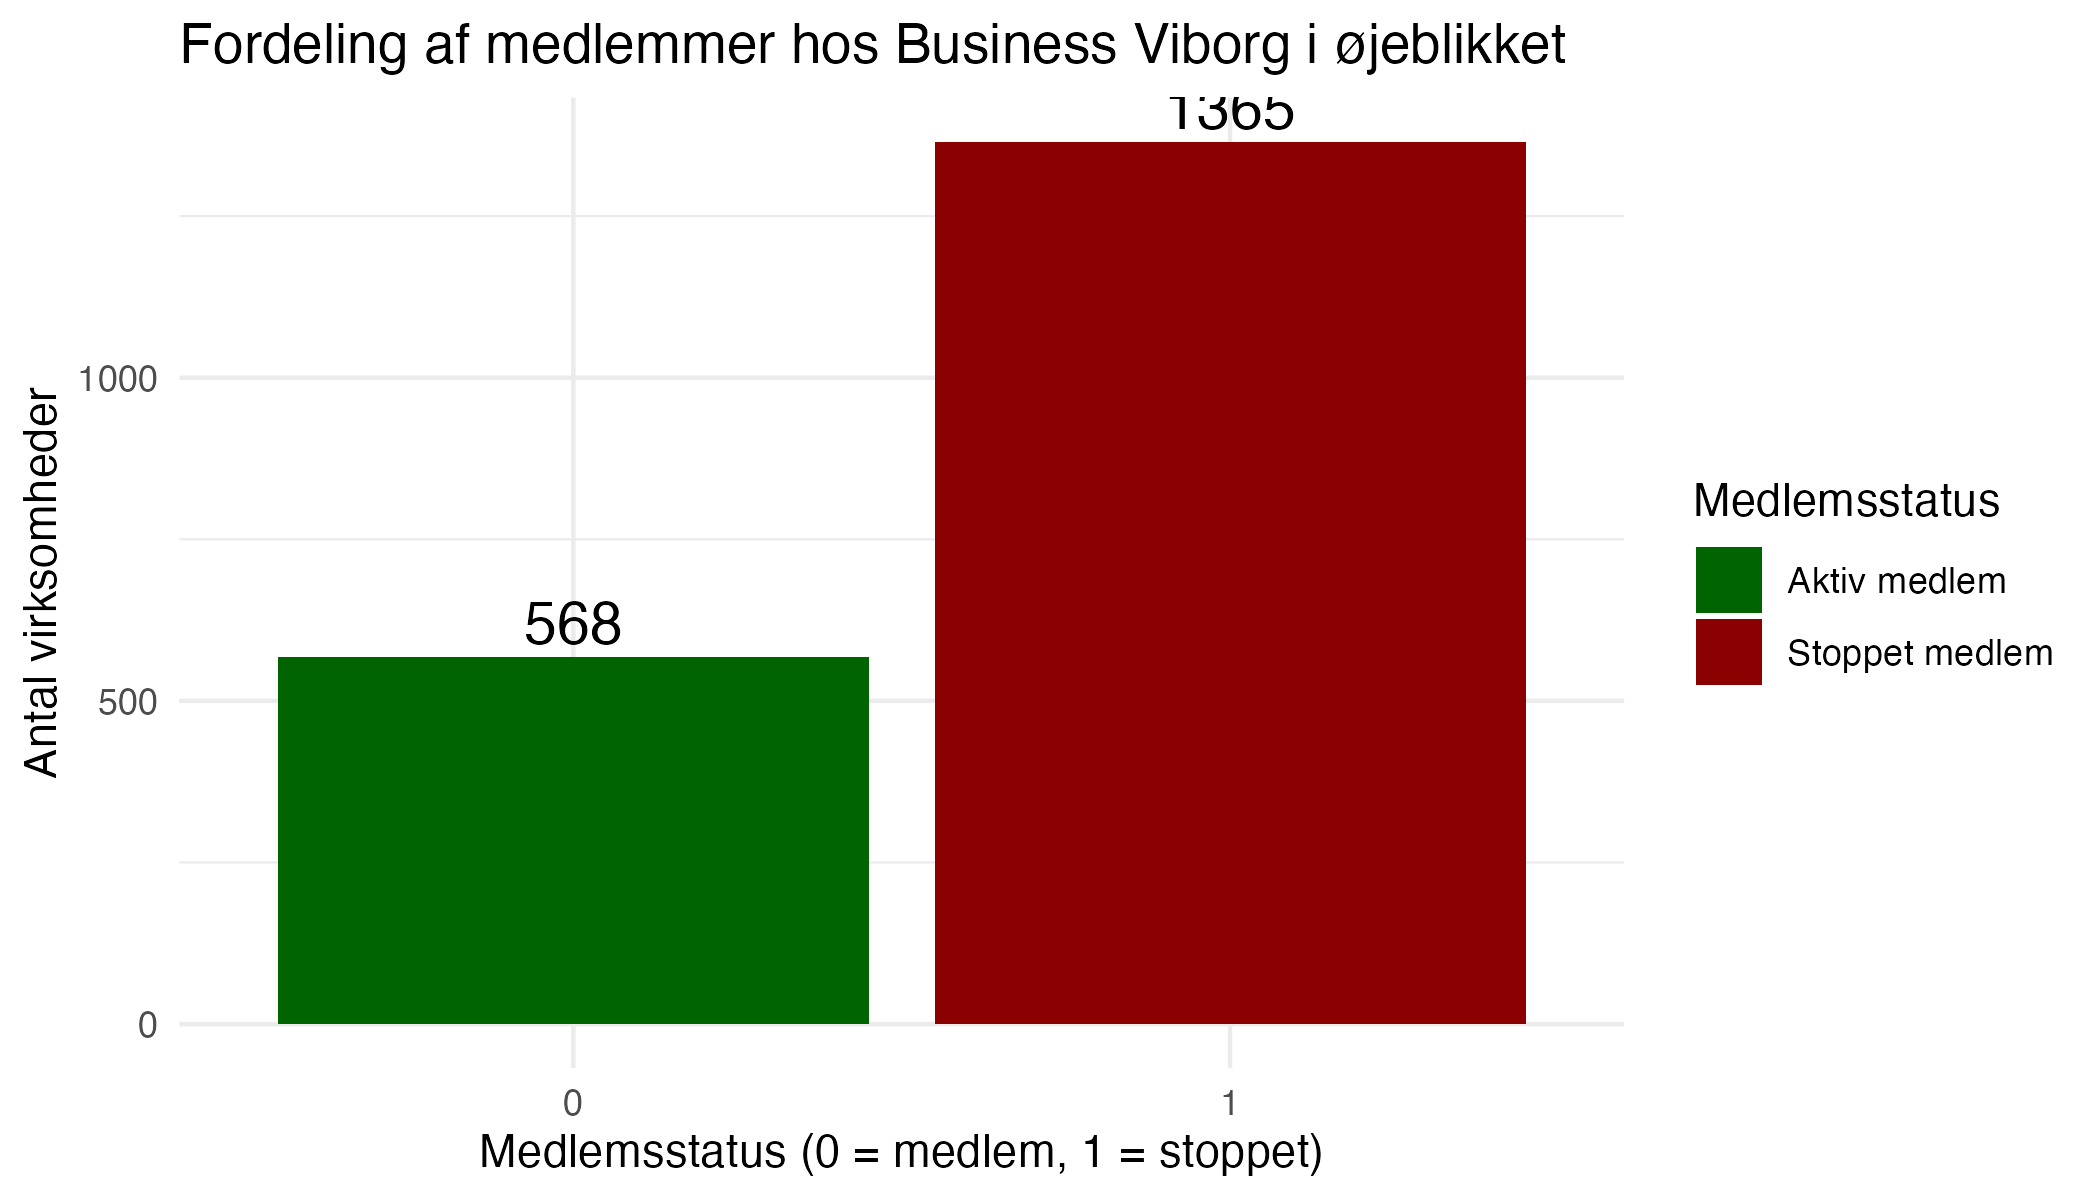
\includegraphics[width=0.8\textwidth,height=\textheight]{images/EDA_1_fordeling_medlemmer.png}
\end{center}

\begin{itemize}
\item
  \textbf{Bilag 2:} Eventdeltagelse blandt aktive medlemmer
  \begin{center}
  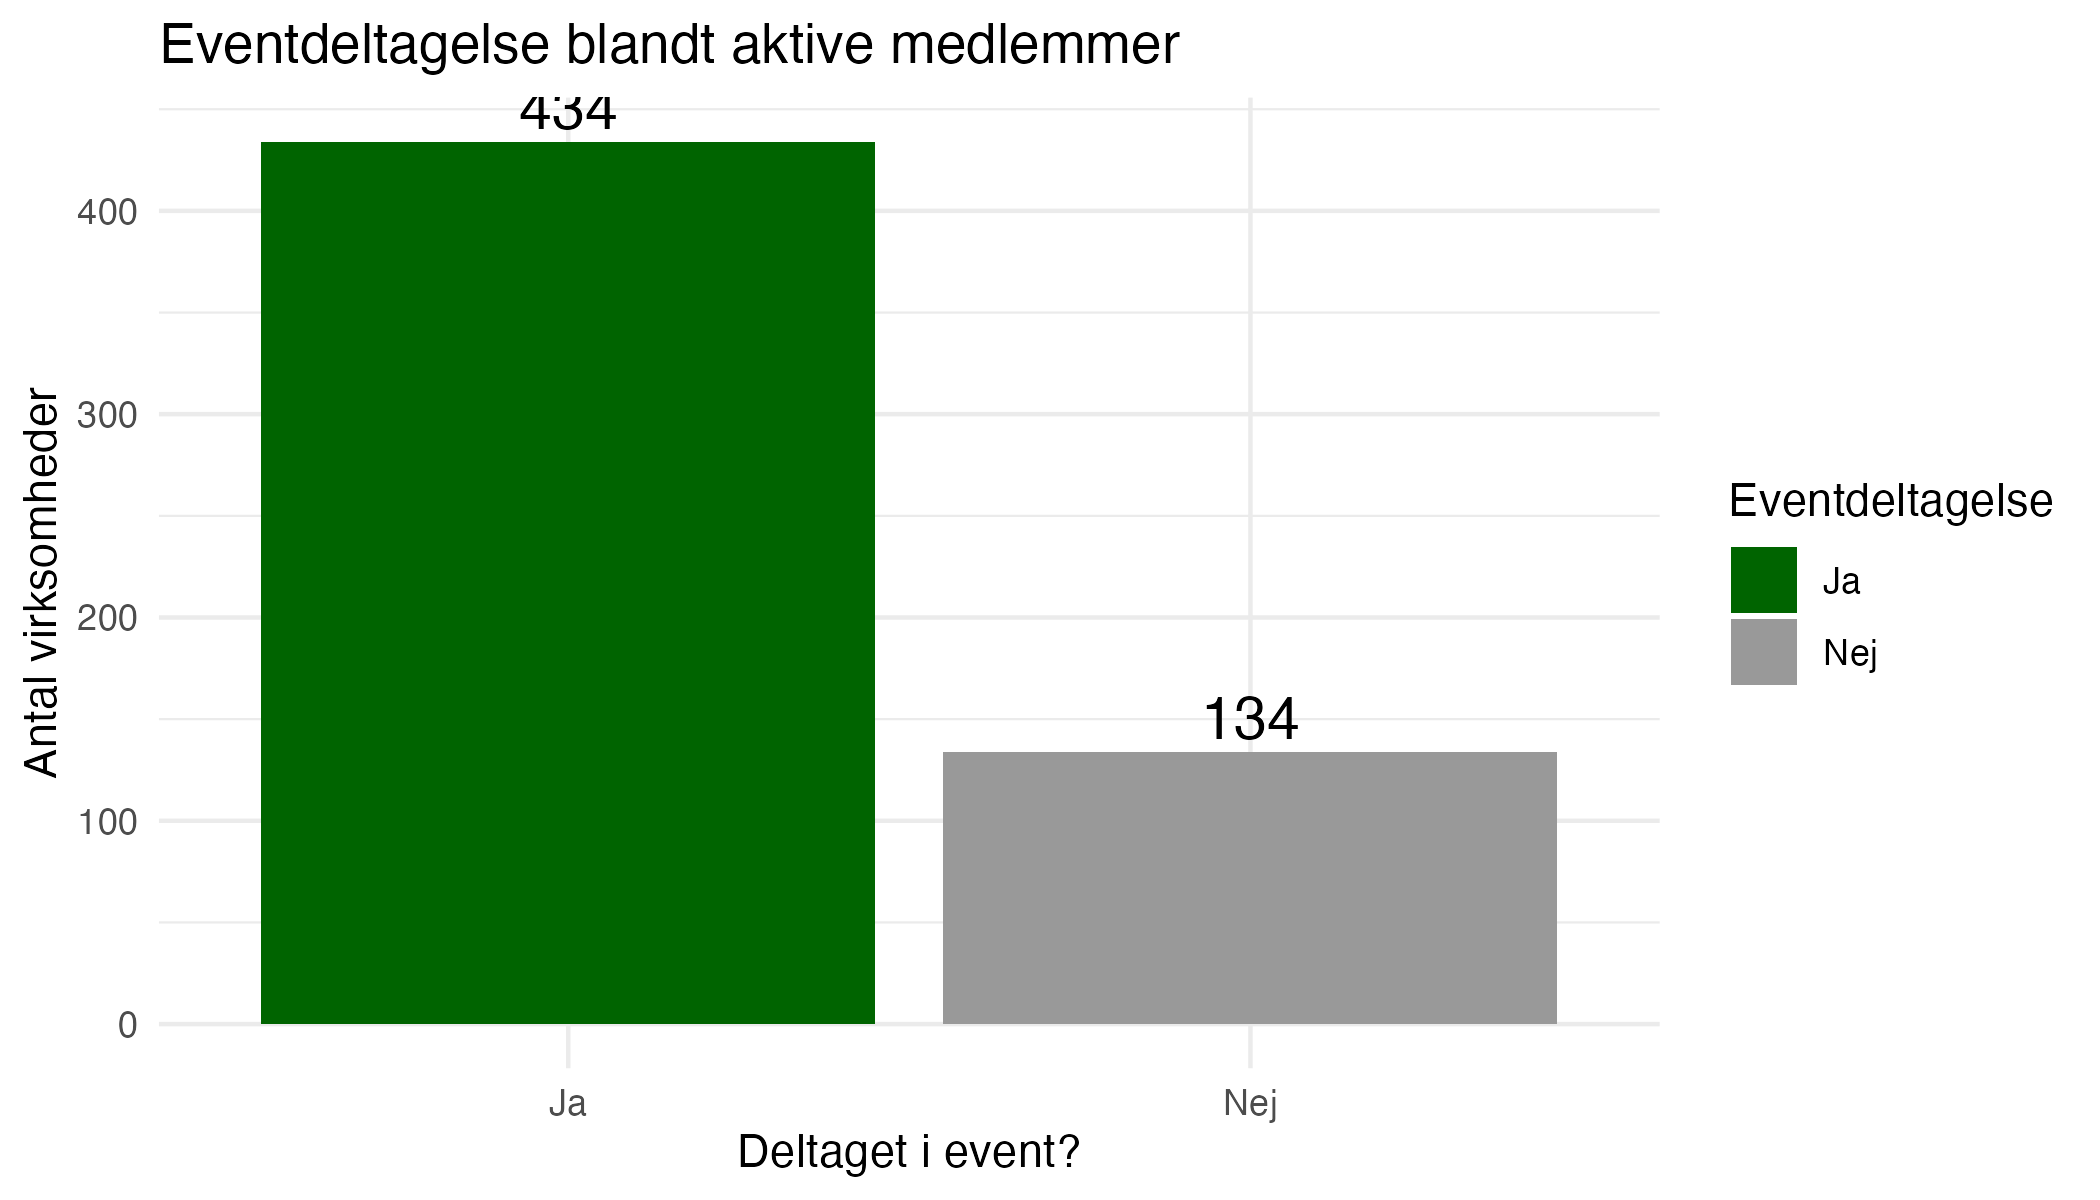
\includegraphics[width=0.8\textwidth,height=\textheight]{images/EDA_2_eventdeltagelse.png}
  \end{center}
\item
  \textbf{Bilag 3:} Branchefordeling blandt aktive medlemmer
  \begin{center}
  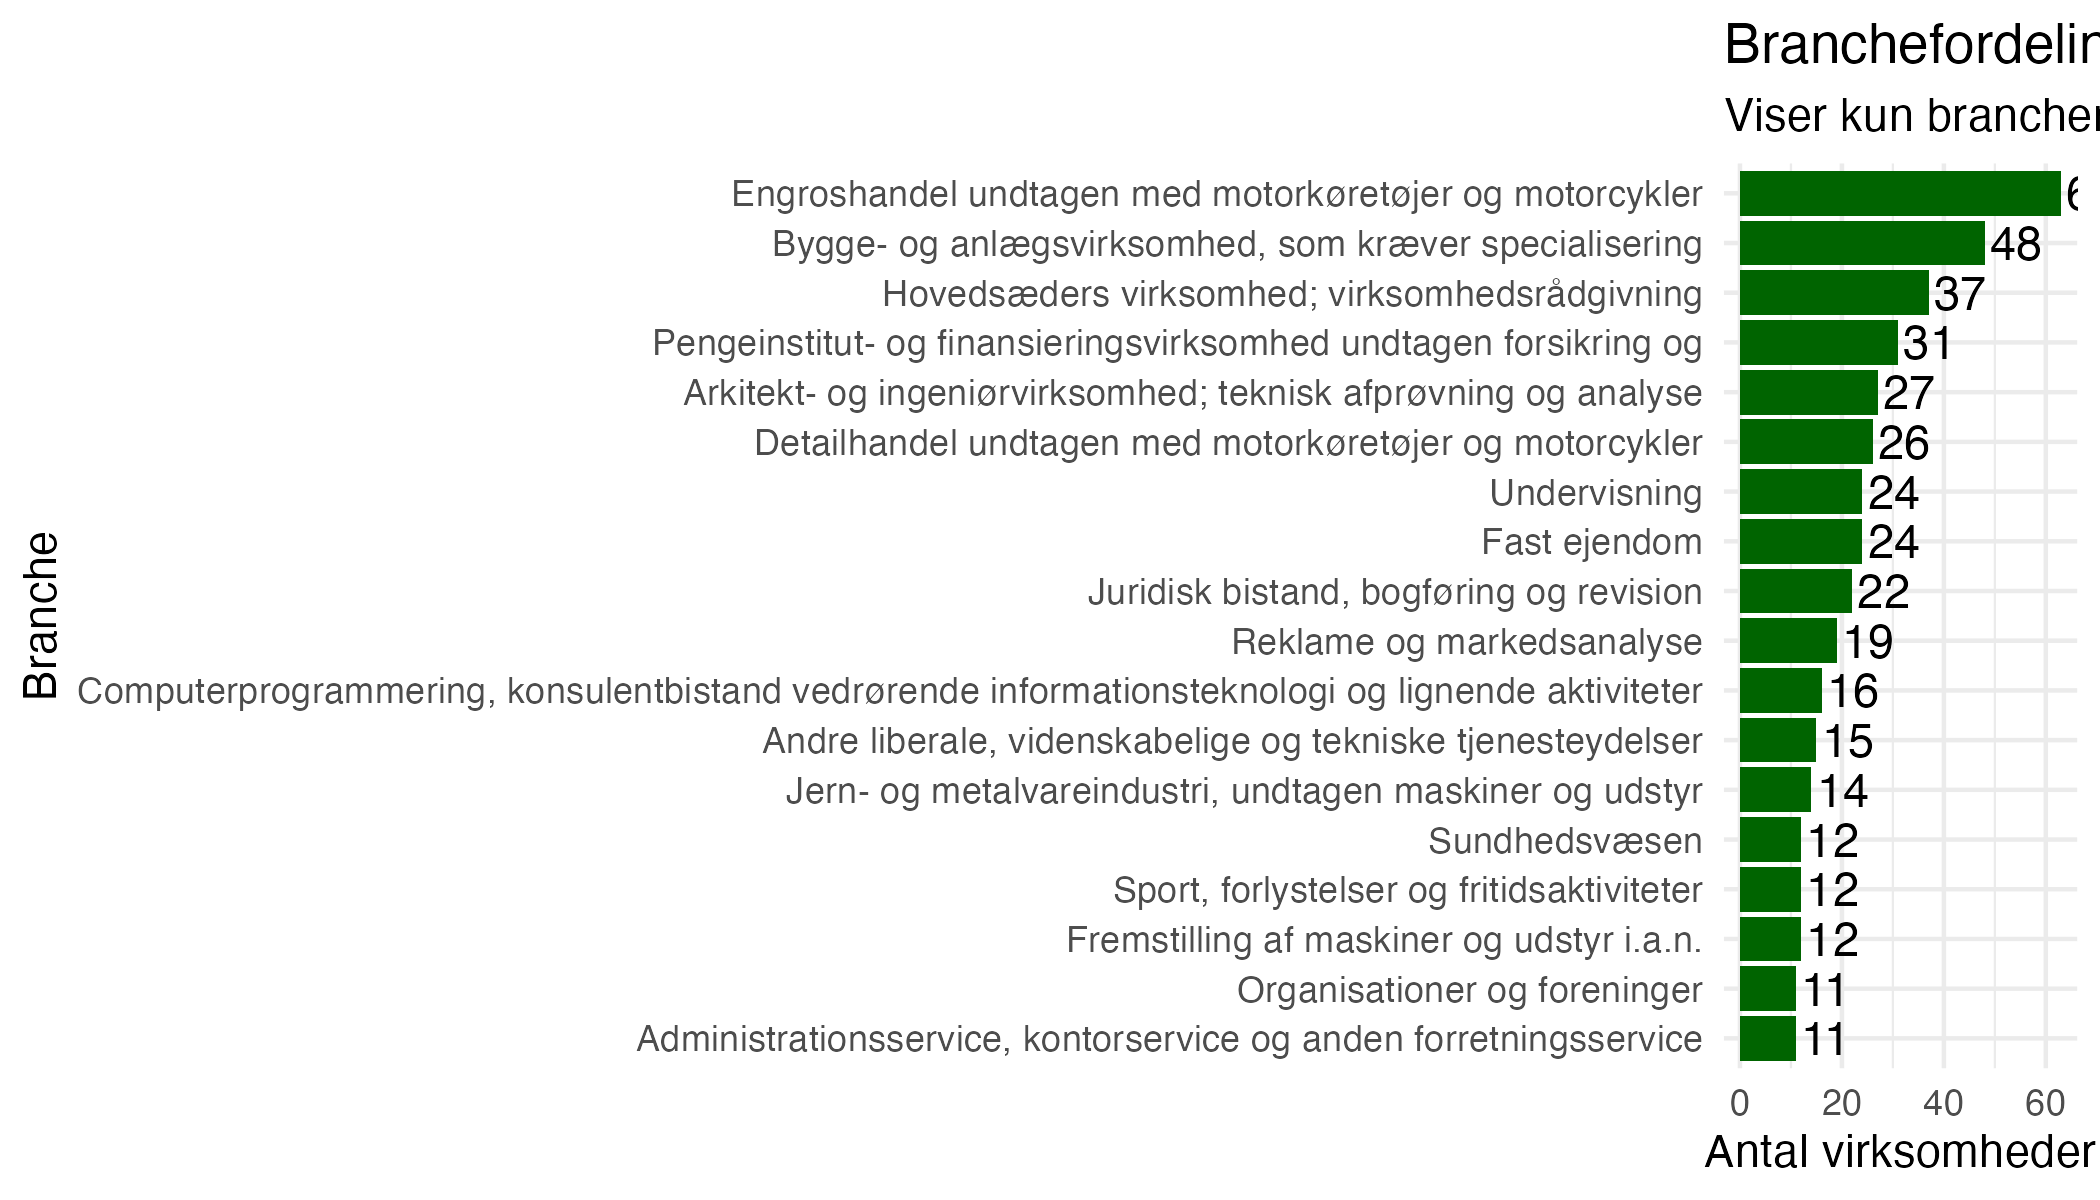
\includegraphics[width=0.8\textwidth,height=\textheight]{images/EDA_4_branchefordeling.png}
  \end{center}
\item
  \textbf{Bilag 4:} Eventdeltagelse pr. postnummer \begin{center}
  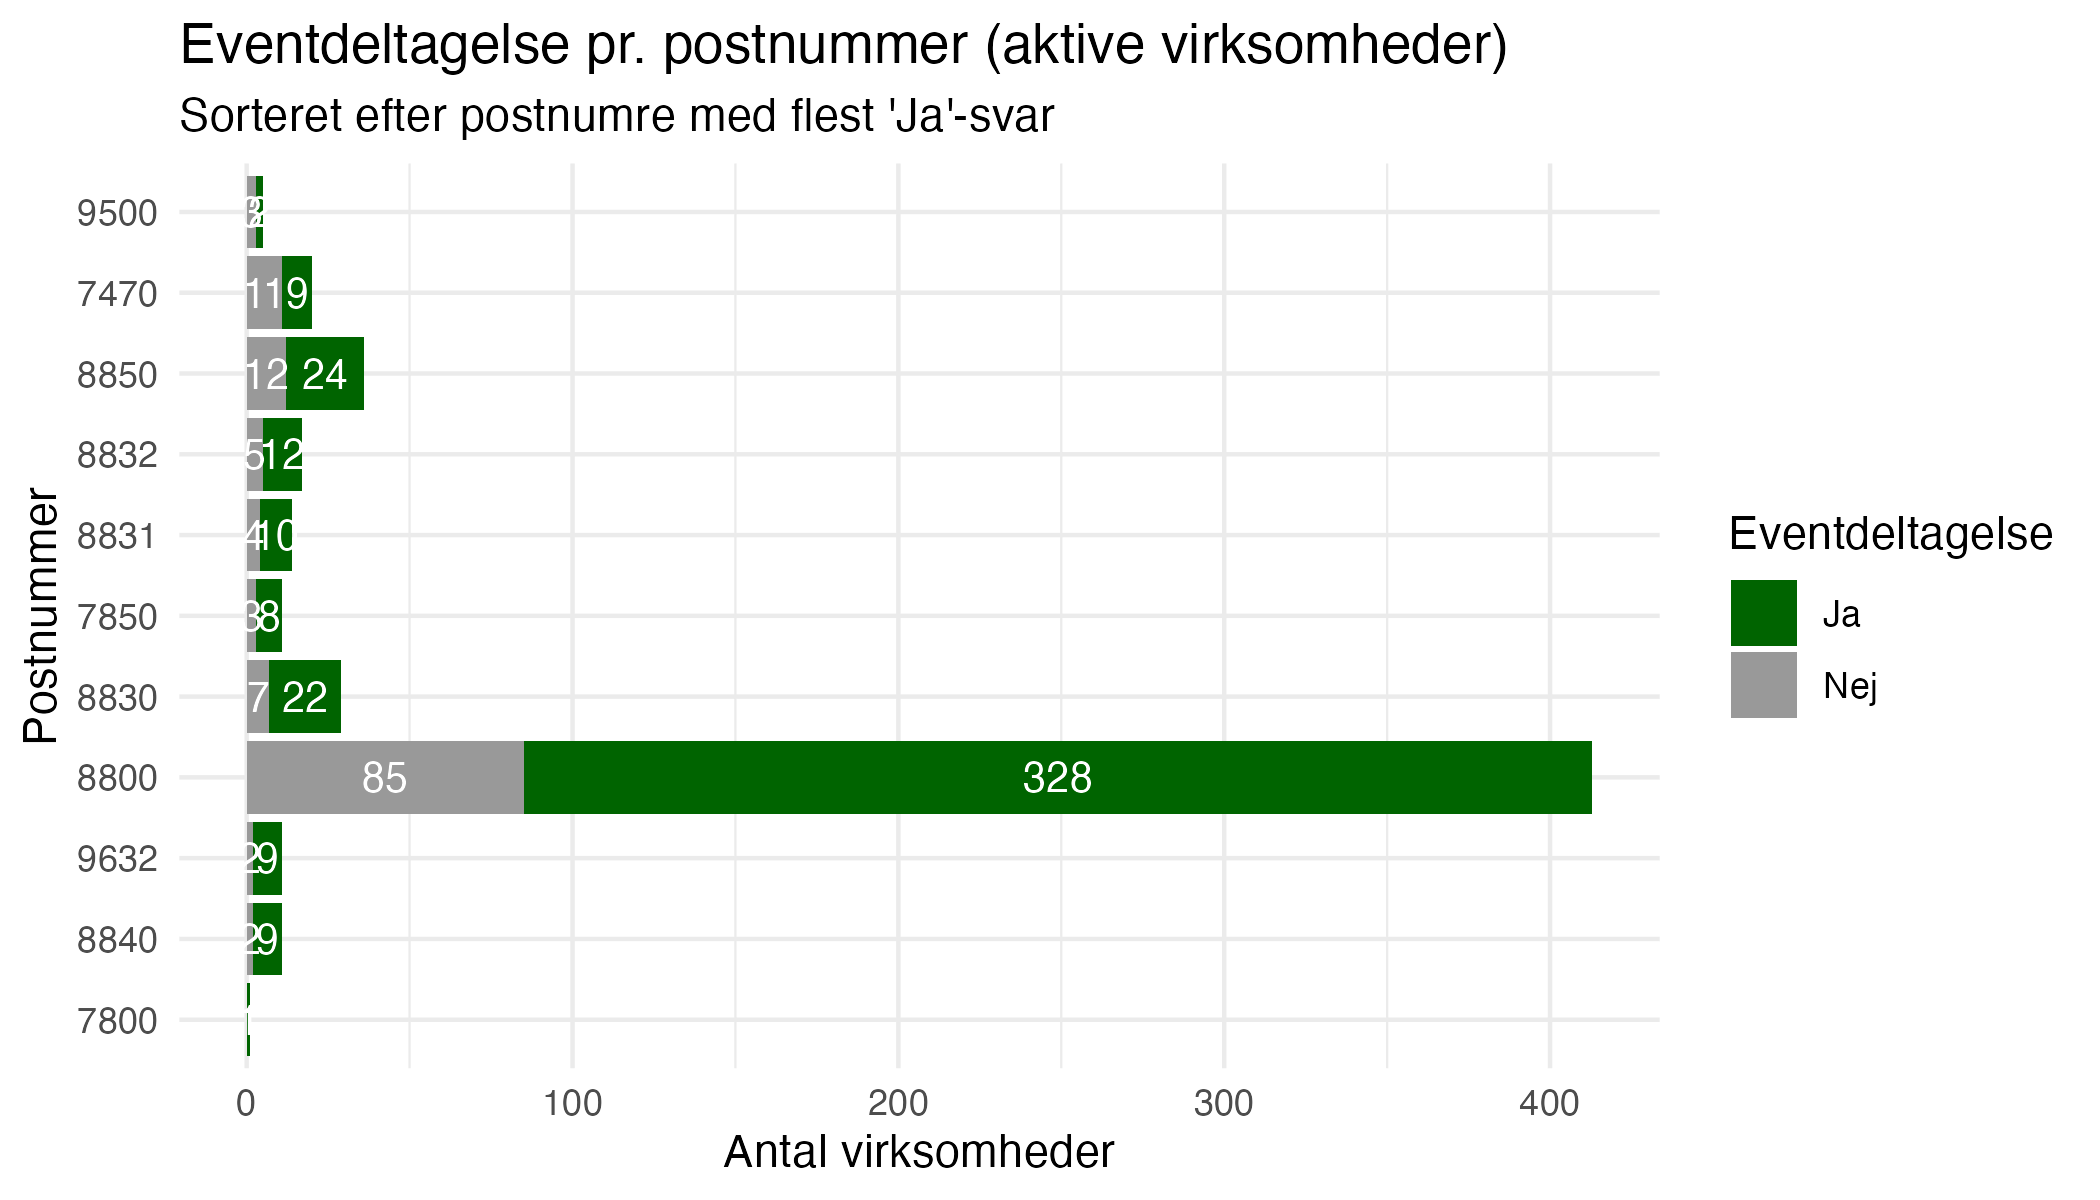
\includegraphics[width=0.8\textwidth,height=\textheight]{images/EDA_5_eventdeltagelse_postnummer.png}
  \end{center}
\item
  \textbf{Bilag 5:} Korrellationsmatrix for numeriske variabler
  \begin{center}
  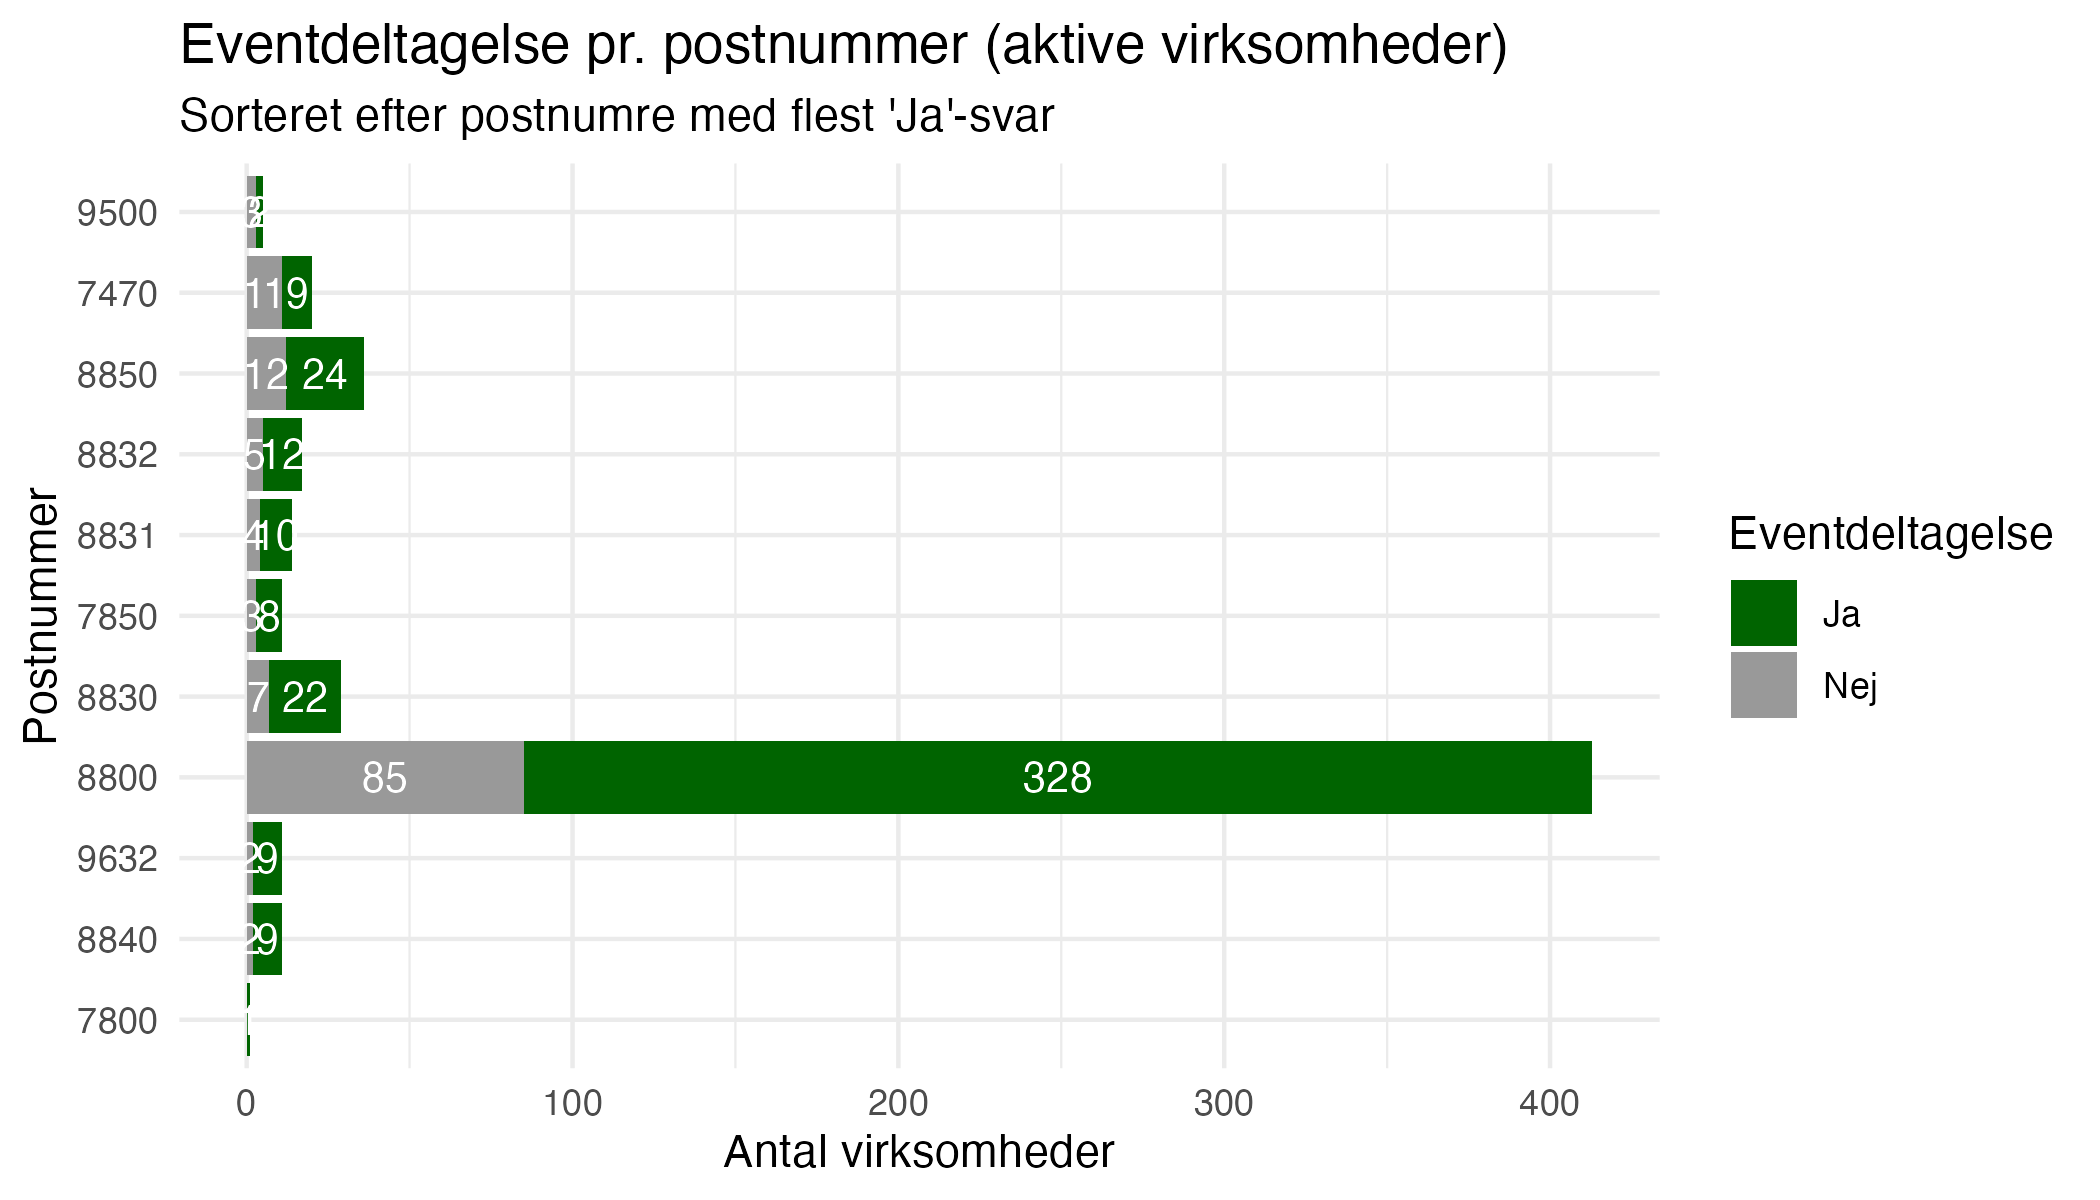
\includegraphics[width=0.8\textwidth,height=\textheight]{images/EDA_6_korrellationsmatrix.png}
  \end{center}
\item
  \textbf{Bilag 6:} Mødelængde vs.~eventdeltagelse\\
  \begin{center}
  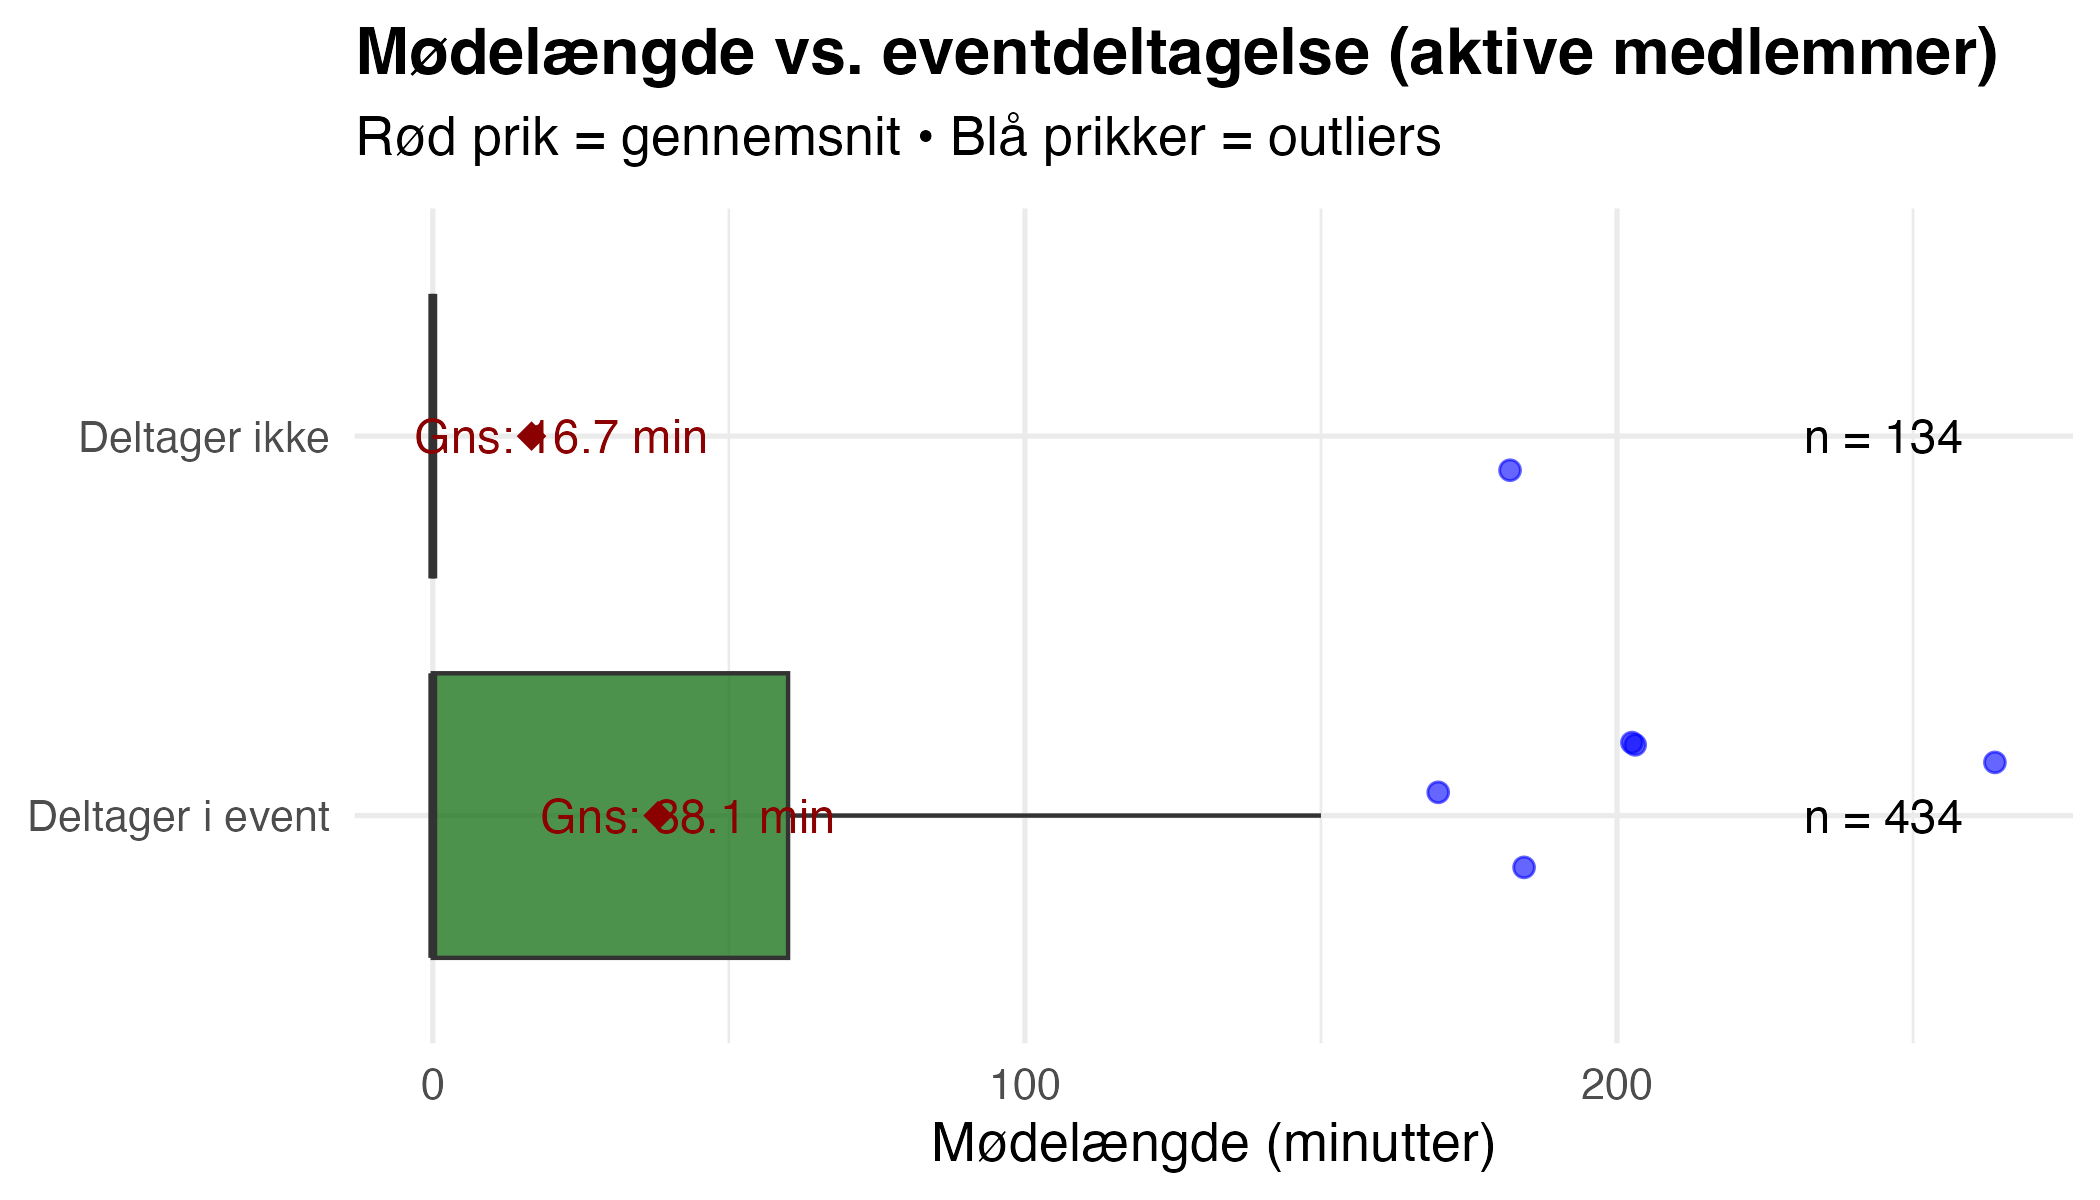
\includegraphics[width=0.8\textwidth,height=\textheight]{images/EDA_7_mødelængde_eventdeltagelse.png}
  \end{center}
\end{itemize}

\subsection{Bilag 7--15: Modeludvikling og
evaluering}\label{bilag-715-modeludvikling-og-evaluering}

Anvendt i forbindelse med udvikling og evaluering af ML-modeller:

\begin{itemize}
\item
  \textbf{Bilag 7:} Model performance (Accuracy, F1 og ROC AUC)\\
  \begin{center}
  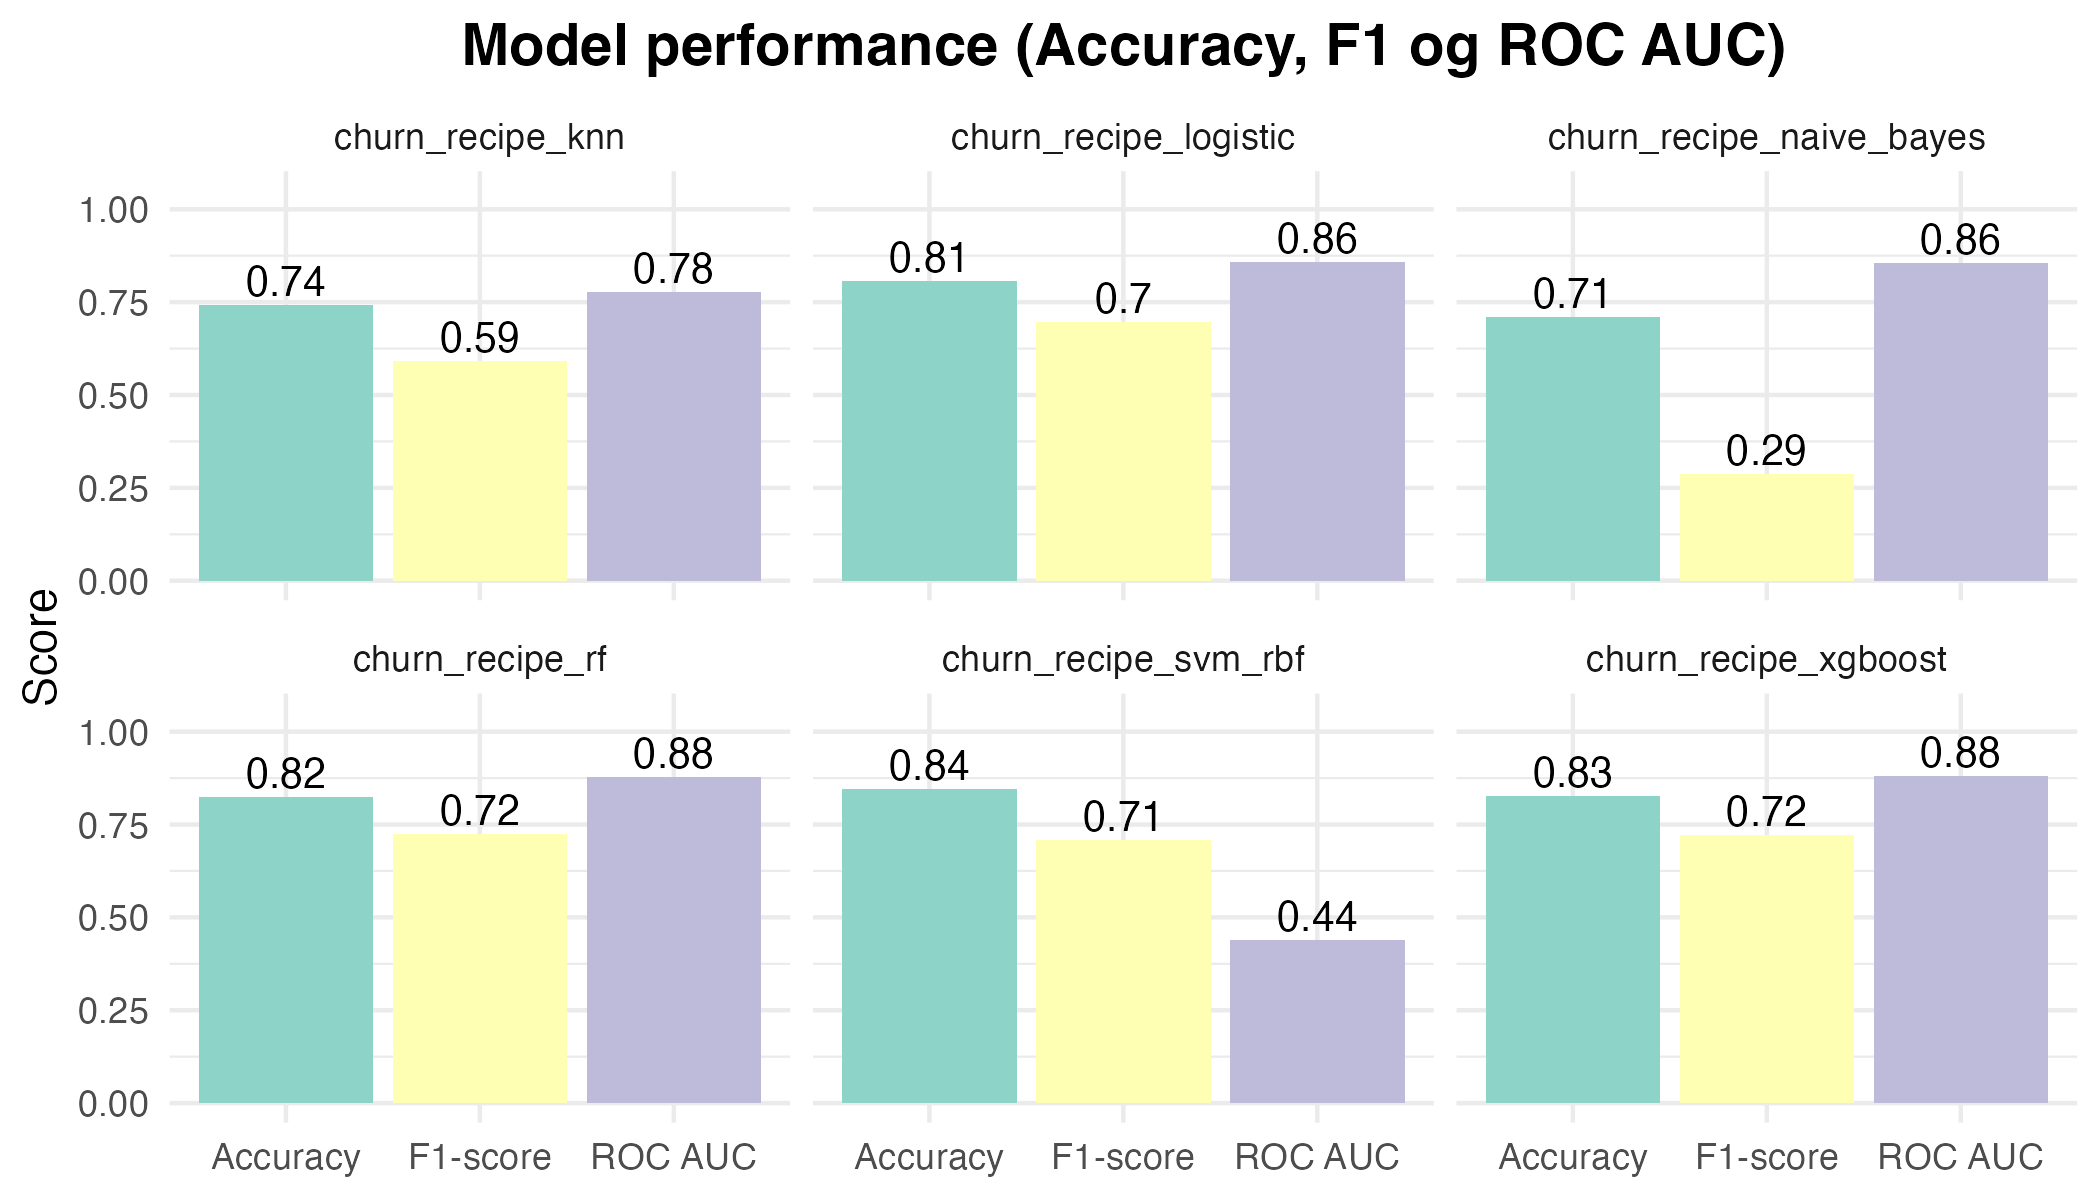
\includegraphics[width=0.8\textwidth,height=\textheight]{images/1_model_performance.png}
  \end{center}
\item
  \textbf{Bilag 8:} Top 10 vigtigste variabler pr. model\\
  \begin{center}
  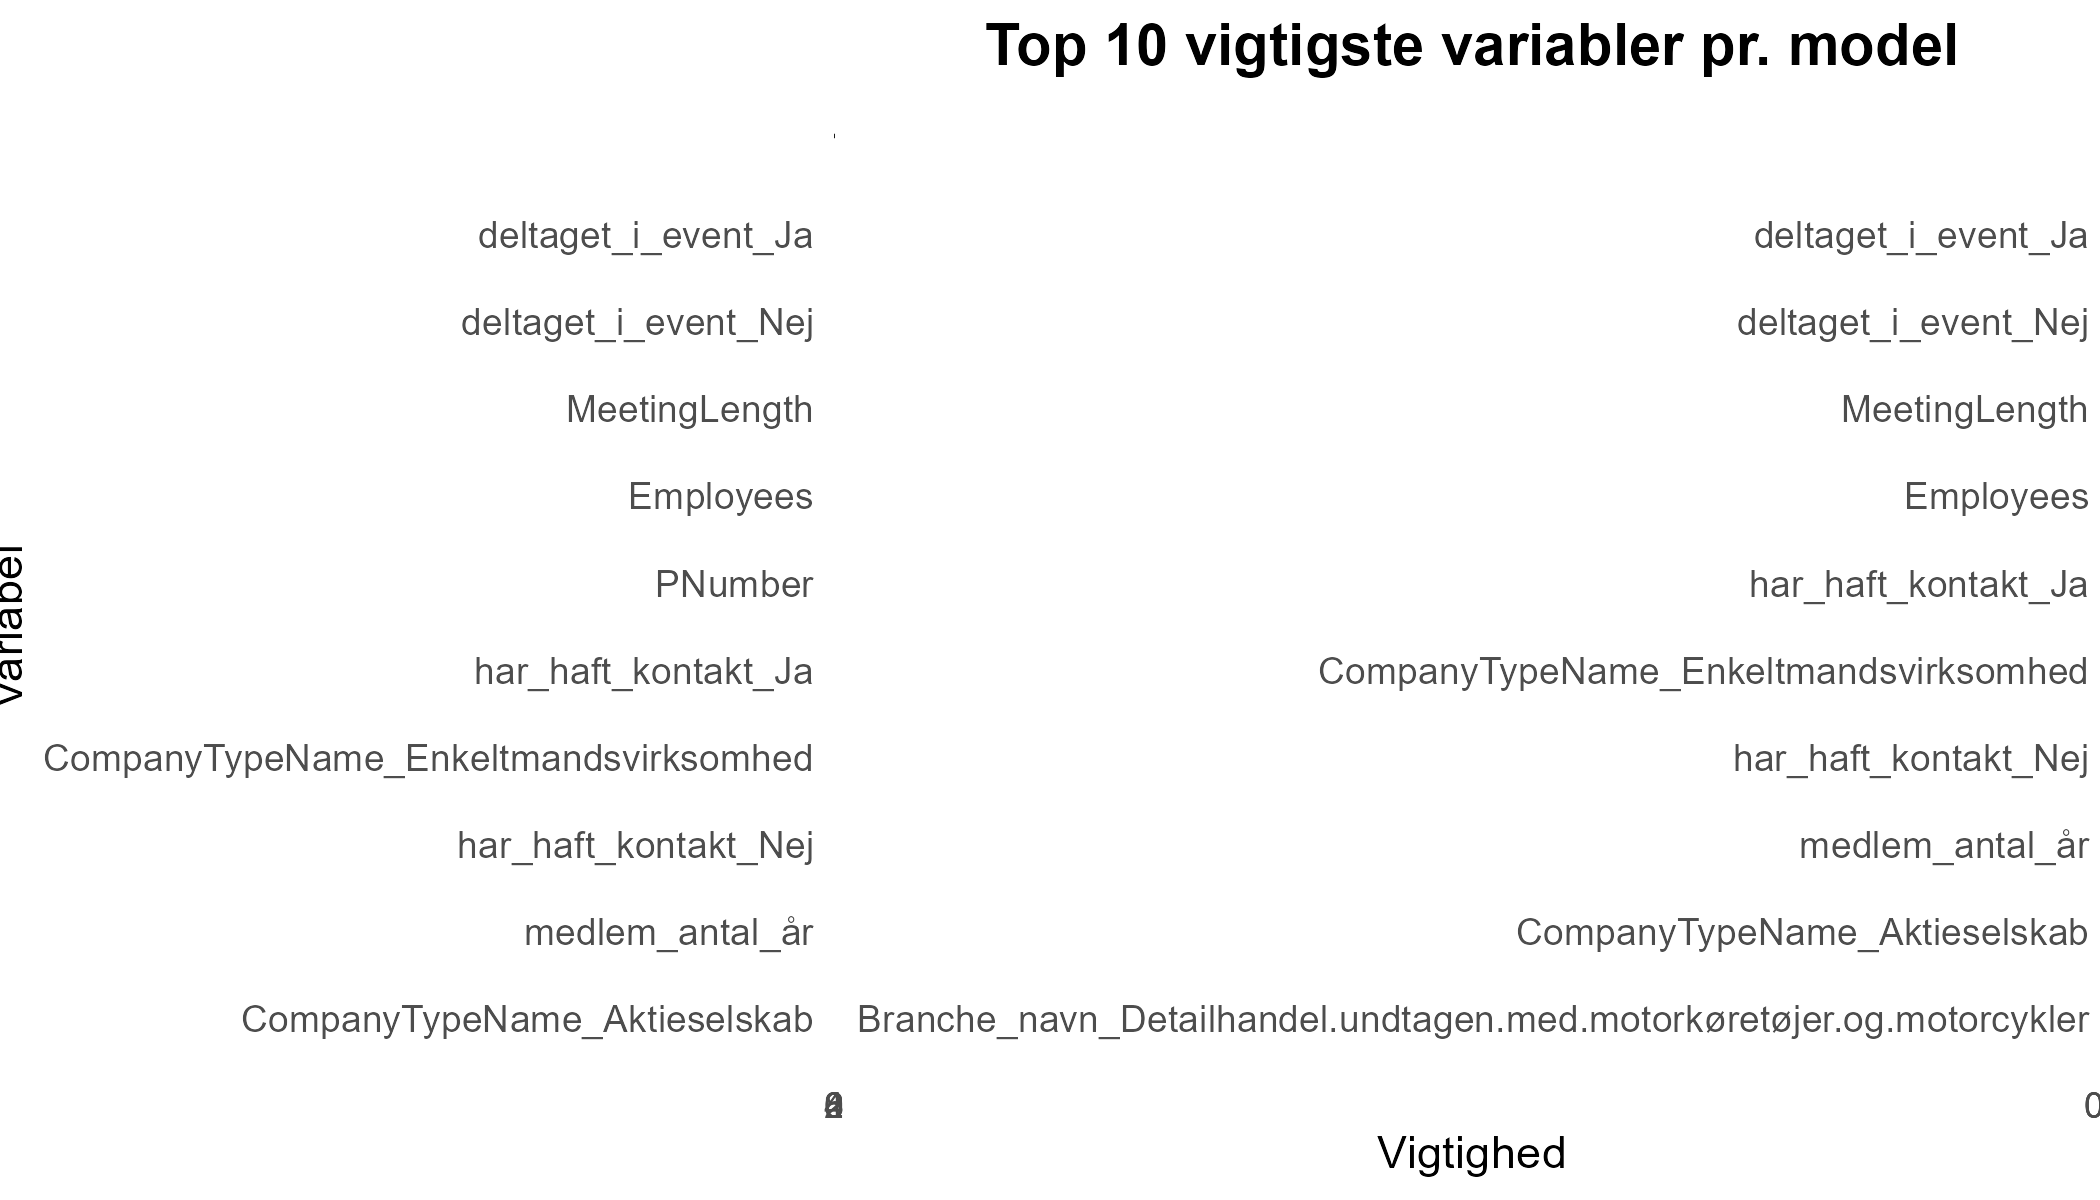
\includegraphics[width=0.8\textwidth,height=\textheight]{images/4_top_10_variabler_pr_model.png}
  \end{center}
\item
  \textbf{Bilag 9:} Sammenlignende heatmap over modeller \begin{center}
  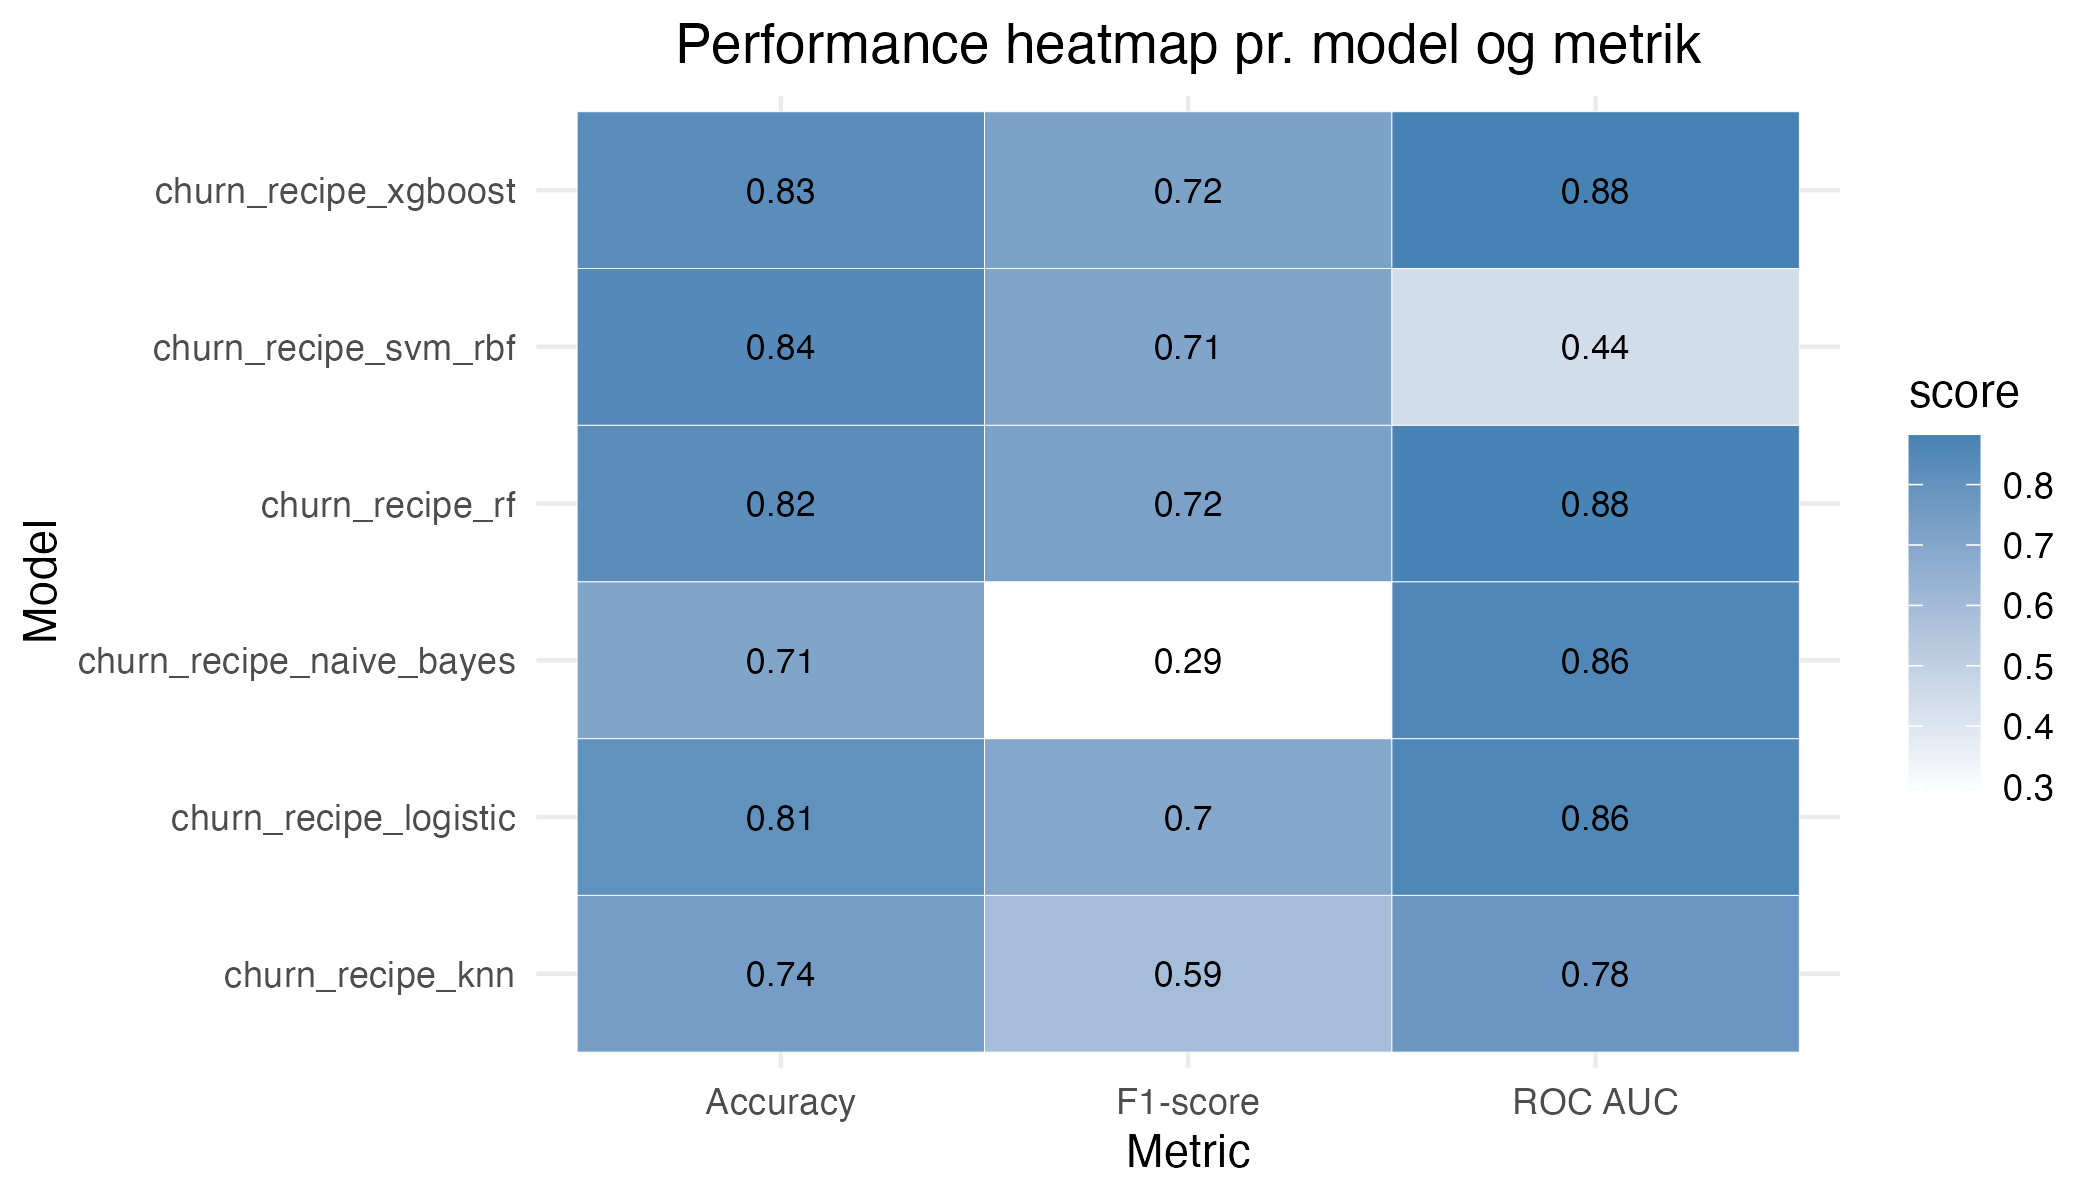
\includegraphics[width=0.8\textwidth,height=\textheight]{images/3_heatmap_pr_model.png}
  \end{center}
\item
  \textbf{Bilag 10:} Udvikling over tid -- churn-risiko \begin{center}
  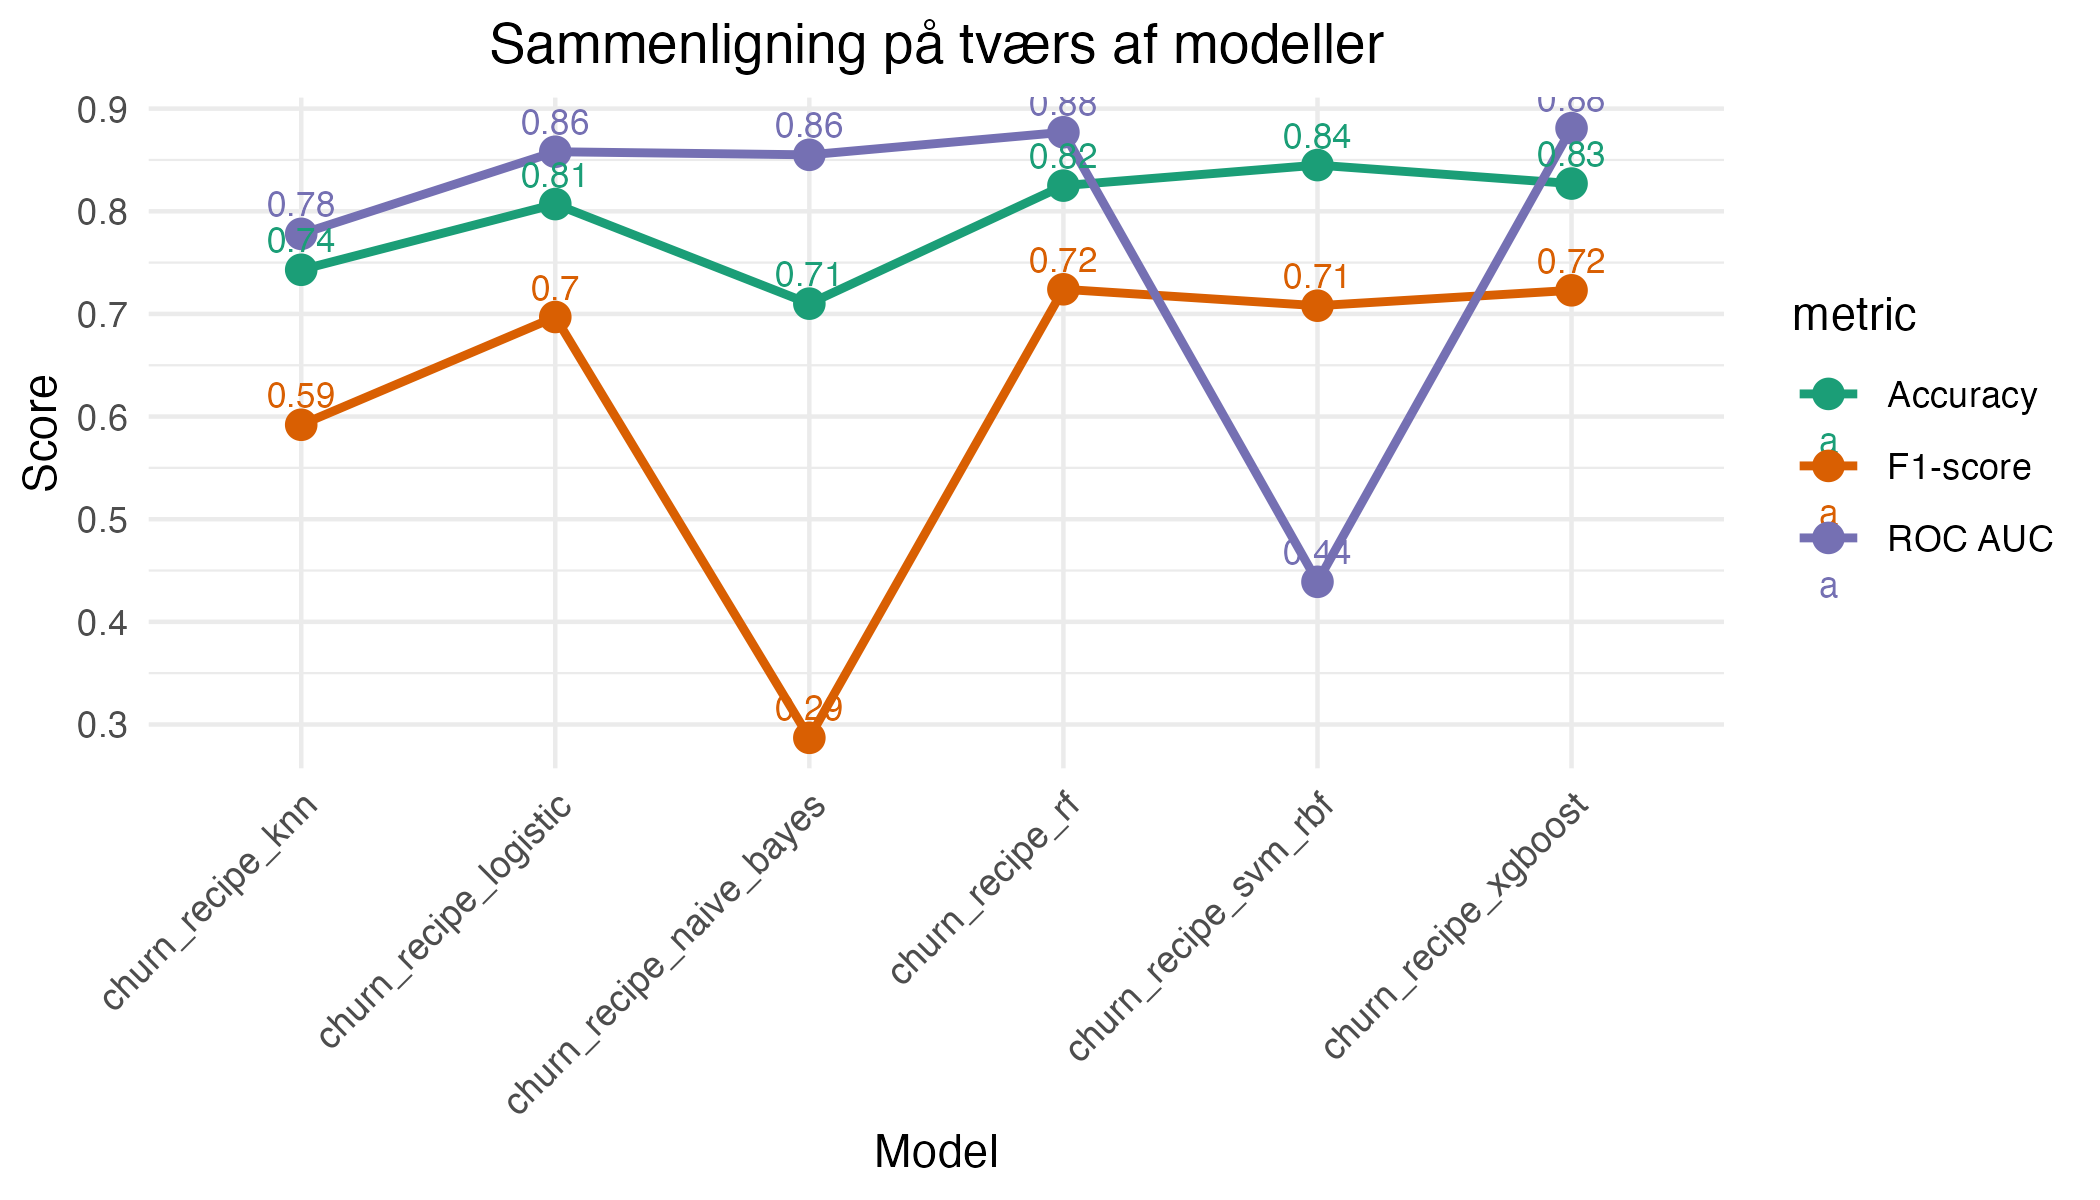
\includegraphics[width=0.8\textwidth,height=\textheight]{images/2_linje_plot.png}
  \end{center}
\item
  \textbf{Bilag 11:} Brancher med højest churn-rate \begin{center}
  \includegraphics[width=0.8\textwidth,height=\textheight]{images/5_brancher_højeste_churn.png}
  \end{center}
\item
  \textbf{Bilag 12:} Postnumre med højest churn-rate \begin{center}
  \includegraphics[width=0.8\textwidth,height=\textheight]{images/6_postnummer_højeste_churn.png}
  \end{center}
\item
  \textbf{Bilag 13:} Top 5 segmenter som ikke churner \begin{center}
  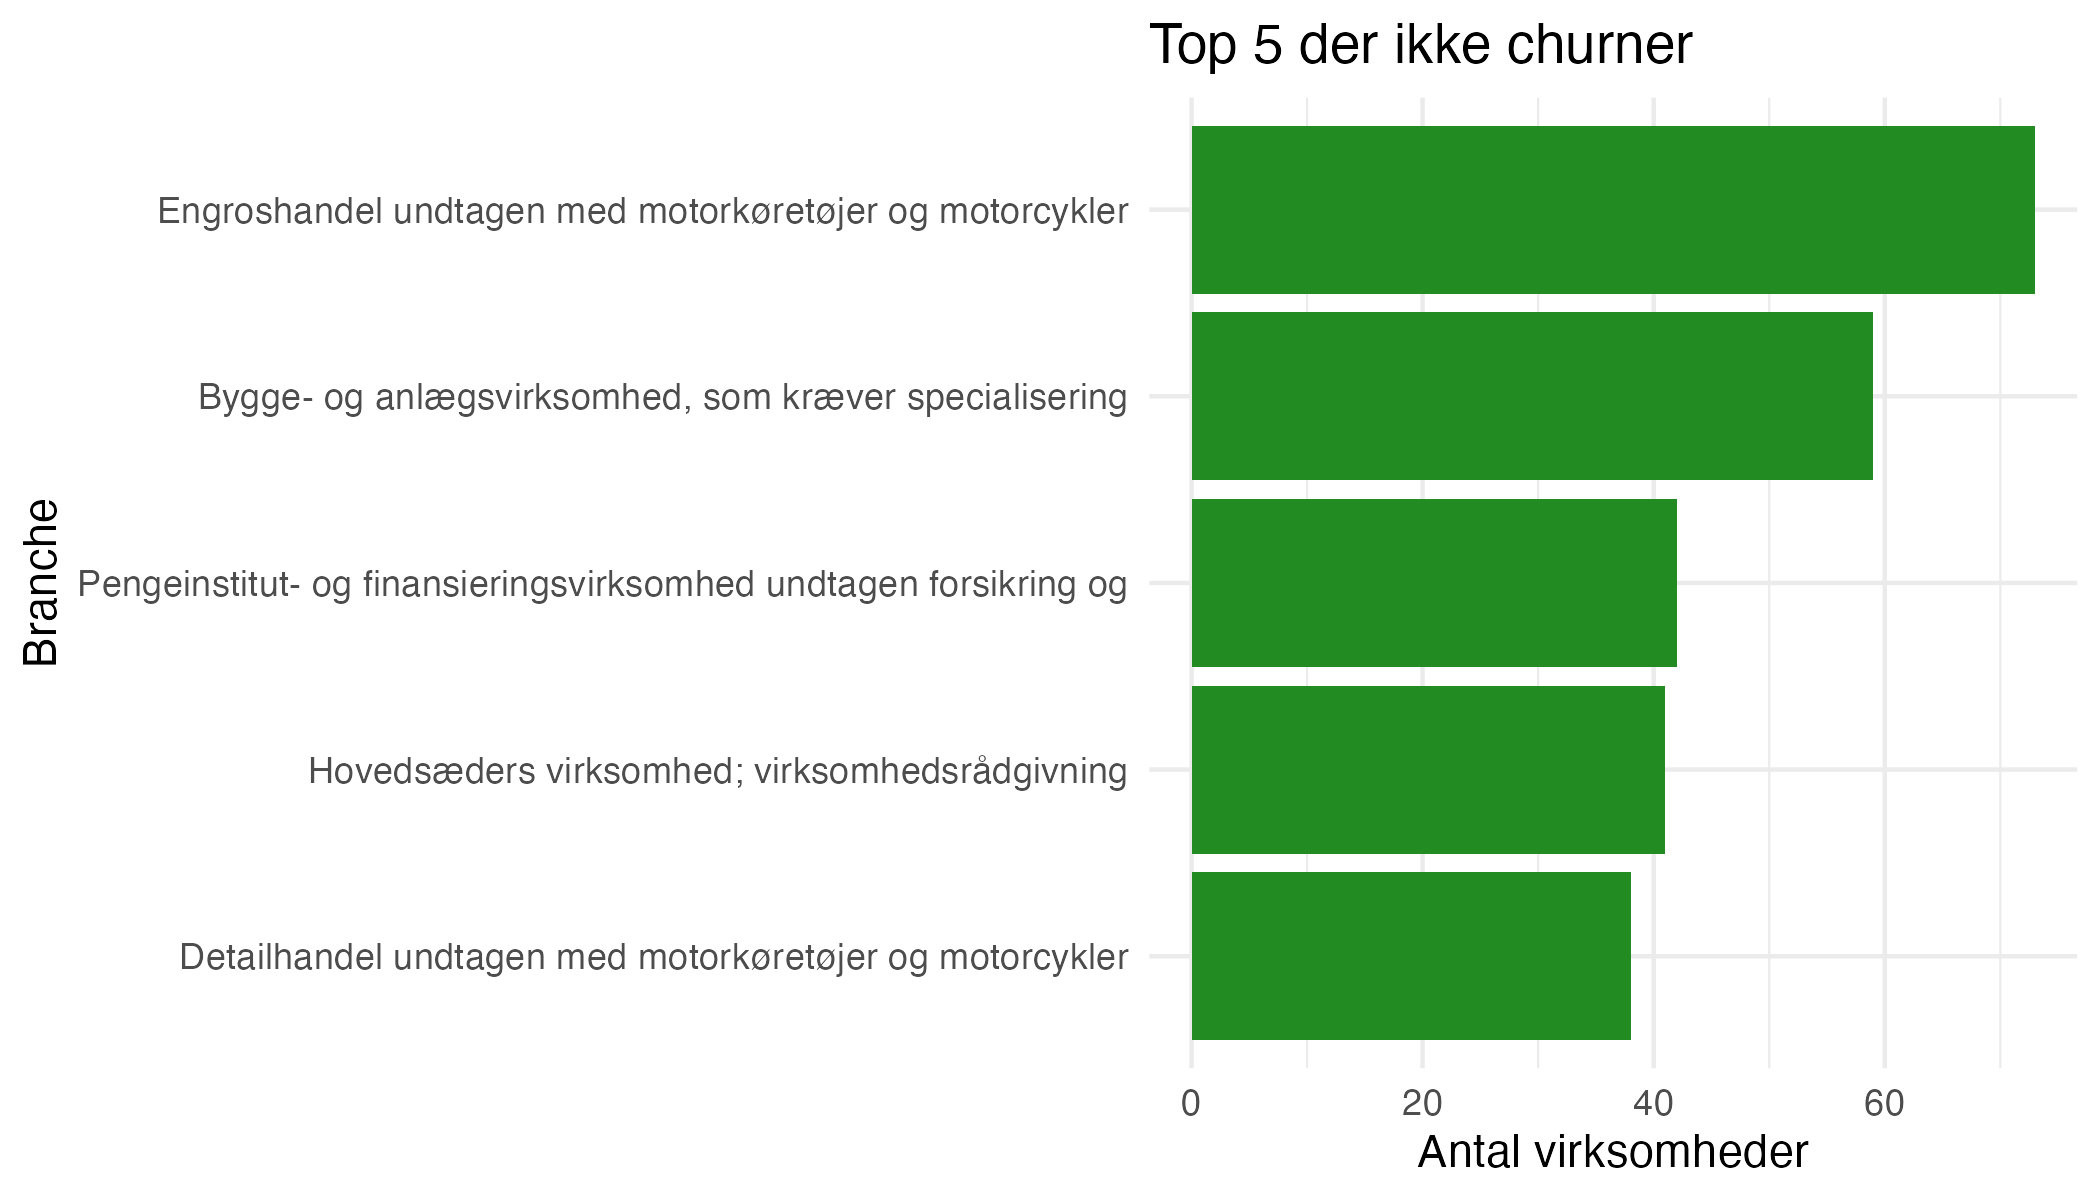
\includegraphics[width=0.8\textwidth,height=\textheight]{images/7_top5_der_ikke_churner.png}
  \end{center}
\item
  \textbf{Bilag 14:} Churn-risikokategorier for aktive kunder
  \begin{center}
  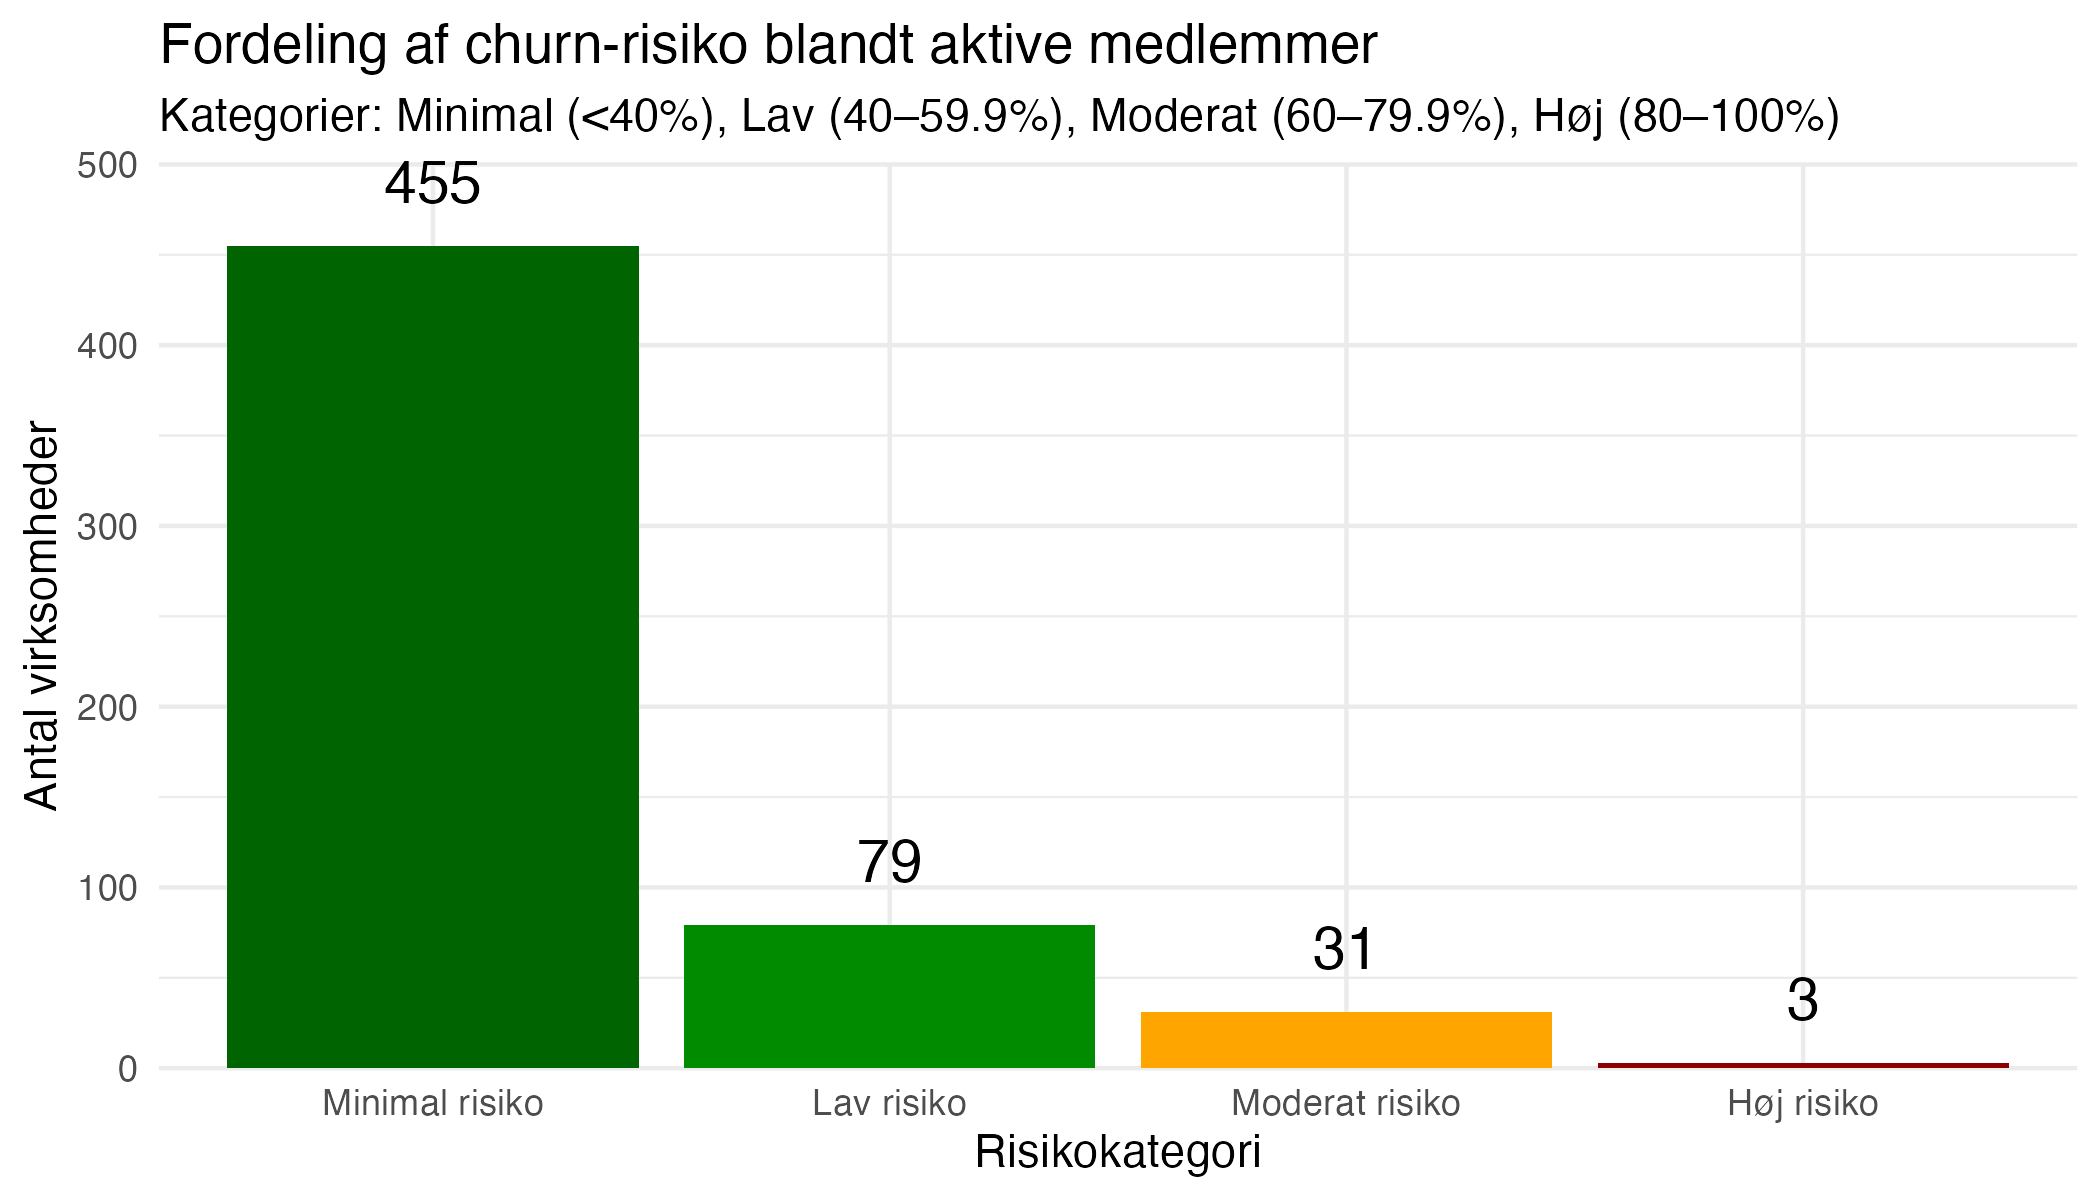
\includegraphics[width=0.8\textwidth,height=\textheight]{images/9_churn_risikokategorier_aktive.png}
  \end{center}
\item
  \textbf{Bilag 15:} Top 10 variable i Random Forest modellen
  \begin{center}
  \includegraphics[width=0.8\textwidth,height=\textheight]{images/8_top_10_variable_rf.png}
  \end{center}
\end{itemize}

\newpage

\begin{Shaded}
\begin{Highlighting}[]
\CommentTok{\# {-}{-}{-}{-}{-}{-}{-}{-}{-}{-}{-}{-}{-}{-}{-}{-}{-}{-}{-}{-}{-}{-}{-}{-}{-}{-}{-}{-}{-}{-}{-}{-}{-}{-}{-}{-}{-}{-}{-}{-}{-}{-}{-}{-}{-}{-}{-}{-}{-}{-}{-}{-}{-}{-}{-}{-}{-}{-}{-}{-}{-}{-}{-}{-}{-}{-}{-}{-}{-}{-}{-}{-}{-}{-}{-}{-}{-}{-}}
\CommentTok{\# 1. Load data}
\CommentTok{\# {-}{-}{-}{-}{-}{-}{-}{-}{-}{-}{-}{-}{-}{-}{-}{-}{-}{-}{-}{-}{-}{-}{-}{-}{-}{-}{-}{-}{-}{-}{-}{-}{-}{-}{-}{-}{-}{-}{-}{-}{-}{-}{-}{-}{-}{-}{-}{-}{-}{-}{-}{-}{-}{-}{-}{-}{-}{-}{-}{-}{-}{-}{-}{-}{-}{-}{-}{-}{-}{-}{-}{-}{-}{-}{-}{-}{-}{-}}

\CommentTok{\# Indlæser alle nødvendige datasæt}
\NormalTok{meetings }\OtherTok{\textless{}{-}} \FunctionTok{readRDS}\NormalTok{(}\StringTok{"data/meetings.rds"}\NormalTok{)}
\NormalTok{events }\OtherTok{\textless{}{-}} \FunctionTok{readRDS}\NormalTok{(}\StringTok{"data/events.rds"}\NormalTok{)}
\NormalTok{event\_participants }\OtherTok{\textless{}{-}} \FunctionTok{readRDS}\NormalTok{(}\StringTok{"data/event\_participants.rds"}\NormalTok{)}
\NormalTok{company\_contacts }\OtherTok{\textless{}{-}} \FunctionTok{readRDS}\NormalTok{(}\StringTok{"data/company\_contacts.rds"}\NormalTok{)}
\NormalTok{all\_contact }\OtherTok{\textless{}{-}} \FunctionTok{readRDS}\NormalTok{(}\StringTok{"data/all\_contact.rds"}\NormalTok{)}
\NormalTok{all\_companies }\OtherTok{\textless{}{-}} \FunctionTok{readRDS}\NormalTok{(}\StringTok{"data/all\_companies.rds"}\NormalTok{)}
\NormalTok{old\_projects }\OtherTok{\textless{}{-}} \FunctionTok{readRDS}\NormalTok{(}\StringTok{"data/old\_projects.rds"}\NormalTok{)}
\end{Highlighting}
\end{Shaded}

\begin{Shaded}
\begin{Highlighting}[]
\CommentTok{\# {-}{-}{-}{-}{-}{-}{-}{-}{-}{-}{-}{-}{-}{-}{-}{-}{-}{-}{-}{-}{-}{-}{-}{-}{-}{-}{-}{-}{-}{-}{-}{-}{-}{-}{-}{-}{-}{-}{-}{-}{-}{-}{-}{-}{-}{-}{-}{-}{-}{-}{-}{-}{-}{-}{-}{-}{-}{-}{-}{-}{-}{-}{-}{-}{-}{-}{-}{-}{-}{-}{-}{-}{-}{-}{-}{-}{-}{-}}
\CommentTok{\# 2. Merge datasets}
\CommentTok{\# {-}{-}{-}{-}{-}{-}{-}{-}{-}{-}{-}{-}{-}{-}{-}{-}{-}{-}{-}{-}{-}{-}{-}{-}{-}{-}{-}{-}{-}{-}{-}{-}{-}{-}{-}{-}{-}{-}{-}{-}{-}{-}{-}{-}{-}{-}{-}{-}{-}{-}{-}{-}{-}{-}{-}{-}{-}{-}{-}{-}{-}{-}{-}{-}{-}{-}{-}{-}{-}{-}{-}{-}{-}{-}{-}{-}{-}{-}}

\CommentTok{\# 2.1: Fjern dubletter og behold første registrering pr. virksomhed}
\NormalTok{meetings\_unique }\OtherTok{\textless{}{-}}\NormalTok{ meetings }\SpecialCharTok{|\textgreater{}}
  \FunctionTok{group\_by}\NormalTok{(CompanyId) }\SpecialCharTok{|\textgreater{}} 
  \FunctionTok{summarise}\NormalTok{(}\FunctionTok{across}\NormalTok{(}\FunctionTok{everything}\NormalTok{(), first))    }\CommentTok{\# Første møde pr. virksomhed}

\NormalTok{events\_unique }\OtherTok{\textless{}{-}}\NormalTok{ events }\SpecialCharTok{|\textgreater{}}
  \FunctionTok{group\_by}\NormalTok{(Cvr) }\SpecialCharTok{|\textgreater{}} 
  \FunctionTok{summarise}\NormalTok{(}\FunctionTok{across}\NormalTok{(}\FunctionTok{everything}\NormalTok{(), first))    }\CommentTok{\# Første event pr. virksomhed}

\NormalTok{event\_participants\_unique }\OtherTok{\textless{}{-}}\NormalTok{ event\_participants }\SpecialCharTok{|\textgreater{}}
  \FunctionTok{group\_by}\NormalTok{(Cvr) }\SpecialCharTok{|\textgreater{}} 
  \FunctionTok{summarise}\NormalTok{(}\FunctionTok{across}\NormalTok{(}\FunctionTok{everything}\NormalTok{(), first))    }\CommentTok{\# Første deltagerinfo pr. virksomhed}


\CommentTok{\# 2.2: Saml alle datasæt med left\_join og ryd op i dubletter}
\NormalTok{merged\_df }\OtherTok{\textless{}{-}}\NormalTok{ all\_companies }\SpecialCharTok{|\textgreater{}} 
  \FunctionTok{left\_join}\NormalTok{(company\_contacts, }\AttributeTok{by =} \StringTok{"CompanyId"}\NormalTok{) }\SpecialCharTok{|\textgreater{}}     \CommentTok{\# Join kontaktpersoner}
  \FunctionTok{left\_join}\NormalTok{(all\_contact, }\AttributeTok{by =} \StringTok{"contactId"}\NormalTok{) }\SpecialCharTok{|\textgreater{}}          \CommentTok{\# Join kontaktinfo}
  \FunctionTok{left\_join}\NormalTok{(meetings\_unique, }\AttributeTok{by =} \StringTok{"CompanyId"}\NormalTok{) }\SpecialCharTok{|\textgreater{}}      \CommentTok{\# Join mødedata}
  \FunctionTok{rename}\NormalTok{(}\AttributeTok{Cvr =} \StringTok{"z\_companies\_1\_CVR{-}nummer\_1"}\NormalTok{) }\SpecialCharTok{|\textgreater{}}        \CommentTok{\# Omdøber kolonnen til }
                                              \CommentTok{\# "Cvr", så den matcher med events}
  \FunctionTok{left\_join}\NormalTok{(events\_unique, }\AttributeTok{by =} \StringTok{"Cvr"}\NormalTok{) }\SpecialCharTok{|\textgreater{}}              \CommentTok{\# Join eventinfo}
  \FunctionTok{left\_join}\NormalTok{(event\_participants\_unique, }\AttributeTok{by =} \StringTok{"Cvr"}\NormalTok{) }\SpecialCharTok{|\textgreater{}}  \CommentTok{\# Join deltagerinfo}
  \FunctionTok{select}\NormalTok{(}\SpecialCharTok{{-}}\FunctionTok{ends\_with}\NormalTok{(}\StringTok{".y"}\NormalTok{), }\SpecialCharTok{{-}}\FunctionTok{ends\_with}\NormalTok{(}\StringTok{".x"}\NormalTok{))           }\CommentTok{\# Fjerner dublet{-}kolonner}


\CommentTok{\# 2.3: Klargør datasæt: fjern anonyme oplysninger og omdøb kolonnenavne}

\CommentTok{\# Fokus: Unikke virksomheder via PNumber (produktionsenhedsnummer)}
\CommentTok{\# Det giver os 2966 unikke observationer.}
\NormalTok{merged\_df }\OtherTok{\textless{}{-}}\NormalTok{ merged\_df }\SpecialCharTok{|\textgreater{}} 
  \FunctionTok{select}\NormalTok{(}\SpecialCharTok{{-}}\NormalTok{z\_companies\_1\_Firmanavn\_1, }\SpecialCharTok{{-}}\NormalTok{z\_contacts\_1\_Email\_1)  }
\CommentTok{\# Fjerner anonymiserede data}

\CommentTok{\# Standardiser kolonnenavne for overskuelighed}
\FunctionTok{colnames}\NormalTok{(merged\_df) }\OtherTok{\textless{}{-}} \FunctionTok{c}\NormalTok{(}
  \StringTok{"BusinessCouncilMember"}\NormalTok{, }\StringTok{"CompanyDateStamp"}\NormalTok{, }\StringTok{"CompanyId"}\NormalTok{, }\StringTok{"CompanyType"}\NormalTok{,}
  \StringTok{"CVR"}\NormalTok{, }\StringTok{"Employees"}\NormalTok{, }\StringTok{"PostalCode"}\NormalTok{, }\StringTok{"CompanyTypeName"}\NormalTok{, }\StringTok{"PNumber"}\NormalTok{, }\StringTok{"Country"}\NormalTok{,}
  \StringTok{"NACECode"}\NormalTok{, }\StringTok{"CompanyStatus"}\NormalTok{, }\StringTok{"AdvertisingProtected"}\NormalTok{, }\StringTok{"ContactId"}\NormalTok{,}
  \StringTok{"CompanyOwnerId"}\NormalTok{, }\StringTok{"ContactLastUpdated"}\NormalTok{, }\StringTok{"TitleChanged"}\NormalTok{, }\StringTok{"LocationChanged"}\NormalTok{,}
  \StringTok{"CreatedBy"}\NormalTok{, }\StringTok{"MeetingLength"}\NormalTok{, }\StringTok{"Firstname"}\NormalTok{, }\StringTok{"UserRole"}\NormalTok{, }\StringTok{"Initials"}\NormalTok{,}
  \StringTok{"EventExternalId"}\NormalTok{, }\StringTok{"EventPublicId"}\NormalTok{, }\StringTok{"Description"}\NormalTok{, }\StringTok{"LocationId"}\NormalTok{,}
  \StringTok{"MaxParticipants"}\NormalTok{, }\StringTok{"EventLength"}\NormalTok{, }\StringTok{"EventId"}
\NormalTok{)}

\CommentTok{\# 2.4: Fjern dubletter og irrelevante kolonner}

\CommentTok{\# Beholder unikke virksomheder, fjerner irrelevante kolonner,}
\CommentTok{\# og udfylder NA i eventdata}
\NormalTok{merged\_unique }\OtherTok{\textless{}{-}}\NormalTok{ merged\_df }\SpecialCharTok{|\textgreater{}}
  \FunctionTok{distinct}\NormalTok{(PNumber, }\AttributeTok{.keep\_all =} \ConstantTok{TRUE}\NormalTok{) }\SpecialCharTok{|\textgreater{}}  \CommentTok{\# Beholder én række pr. PNumber}
  \FunctionTok{select}\NormalTok{(}\SpecialCharTok{{-}}\NormalTok{TitleChanged, }\SpecialCharTok{{-}}\NormalTok{LocationChanged, }\SpecialCharTok{{-}}\NormalTok{CreatedBy, }\SpecialCharTok{{-}}\NormalTok{Firstname,  }
         \CommentTok{\# Fjerner irrelevante variabler}
         \SpecialCharTok{{-}}\NormalTok{UserRole, }\SpecialCharTok{{-}}\NormalTok{Initials, }\SpecialCharTok{{-}}\NormalTok{ContactLastUpdated) }\SpecialCharTok{|\textgreater{}}
  \FunctionTok{mutate}\NormalTok{(}\FunctionTok{across}\NormalTok{(  }\CommentTok{\# Erstatter NA i event{-}kolonner med "Ingen event"}
    \FunctionTok{c}\NormalTok{(MeetingLength, EventExternalId, EventPublicId, Description, }
\NormalTok{      LocationId, MaxParticipants, EventLength, EventId),}
    \SpecialCharTok{\textasciitilde{}} \FunctionTok{if\_else}\NormalTok{(}\FunctionTok{is.na}\NormalTok{(.), }\StringTok{"Ingen event"}\NormalTok{, }\FunctionTok{as.character}\NormalTok{(.))}
\NormalTok{  ))}

\CommentTok{\# Rens MeetingLength og konverter til numerisk (fjern " mins")}
\NormalTok{merged\_unique }\OtherTok{\textless{}{-}}\NormalTok{ merged\_unique }\SpecialCharTok{|\textgreater{}} 
  \FunctionTok{mutate}\NormalTok{(}
    \AttributeTok{MeetingLength =} \FunctionTok{ifelse}\NormalTok{(MeetingLength }\SpecialCharTok{==} \StringTok{"Ingen event"}\NormalTok{, }\StringTok{"0 mins"}\NormalTok{, }
\NormalTok{                           MeetingLength), }
    \AttributeTok{MeetingLength =} \FunctionTok{as.numeric}\NormalTok{(}\FunctionTok{str\_remove}\NormalTok{(MeetingLength, }\StringTok{" mins"}\NormalTok{))}
\NormalTok{  )}

\CommentTok{\# 2.5: Splitter NACECode i kode og beskrivelse, }
\CommentTok{\# fjern original kolonne og NA{-}rækker}

\NormalTok{merged\_unique }\OtherTok{\textless{}{-}}\NormalTok{ merged\_unique }\SpecialCharTok{|\textgreater{}}
  \FunctionTok{mutate}\NormalTok{(}
    \AttributeTok{Employees   =} \FunctionTok{if\_else}\NormalTok{(}\FunctionTok{is.na}\NormalTok{(Employees), }\StringTok{"Ukendt"}\NormalTok{, }\FunctionTok{as.character}\NormalTok{(Employees)),}
    \CommentTok{\# NA {-}\textgreater{} "Ukendt"}
    
    \AttributeTok{NACECode    =} \FunctionTok{if\_else}\NormalTok{(}\FunctionTok{is.na}\NormalTok{(NACECode),  }\StringTok{"Ukendt"}\NormalTok{, }\FunctionTok{as.character}\NormalTok{(NACECode)),}
    \CommentTok{\# NA {-}\textgreater{} "Ukendt"}
    
    \AttributeTok{Nacecode    =} \FunctionTok{if\_else}\NormalTok{(NACECode }\SpecialCharTok{==} \StringTok{"Ukendt"}\NormalTok{, }\StringTok{"Ukendt"}\NormalTok{, }
                          \FunctionTok{str\_extract}\NormalTok{(NACECode, }\StringTok{"\^{}[0{-}9]+"}\NormalTok{)),                 }
    \CommentTok{\# Hent kode}
    \AttributeTok{Nacebranche =} \FunctionTok{if\_else}\NormalTok{(NACECode }\SpecialCharTok{==} \StringTok{"Ukendt"}\NormalTok{, }\StringTok{"Ukendt"}\NormalTok{, }
                          \FunctionTok{str\_remove}\NormalTok{(NACECode, }\StringTok{"\^{}[0{-}9]+}\SpecialCharTok{\textbackslash{}\textbackslash{}}\StringTok{s*"}\NormalTok{))               }
    \CommentTok{\# Hent branche}
\NormalTok{  ) }\SpecialCharTok{|\textgreater{}}
  \FunctionTok{select}\NormalTok{(}\SpecialCharTok{{-}}\NormalTok{NACECode) }\SpecialCharTok{|\textgreater{}}  \CommentTok{\# Fjerner original NACECode{-}kolonne}
  \FunctionTok{na.omit}\NormalTok{()             }\CommentTok{\# Fjerner rækker med NA{-}værdier}

\CommentTok{\# 2.6: Tjek for tilbageværende NA{-}værdier}
\CommentTok{\# colSums(is.na(merged\_unique))}


\CommentTok{\# 2.7: Gem det rensede datasæt til senere brug}

\FunctionTok{saveRDS}\NormalTok{(merged\_unique, }\StringTok{"merged\_unique.rds"}\NormalTok{)}

\CommentTok{\# 2.8: Merge old\_projects (frivillig) med virksomhedsdata}

\CommentTok{\# Omdøb SMVContactId til ContactId}
\NormalTok{old\_projects }\OtherTok{\textless{}{-}}\NormalTok{ old\_projects }\SpecialCharTok{|\textgreater{}}
  \FunctionTok{rename}\NormalTok{(}\AttributeTok{ContactId =}\NormalTok{ SMVContactId) }\CommentTok{\# Omdøb kolonne for at matche join}

\CommentTok{\# Gem kolonnenavne fra old\_projects (ekskl. ContactId)}
\NormalTok{old\_project\_cols }\OtherTok{\textless{}{-}} \FunctionTok{setdiff}\NormalTok{(}\FunctionTok{names}\NormalTok{(old\_projects), }\StringTok{"ContactId"}\NormalTok{)}
\NormalTok{cols\_to\_fill }\OtherTok{\textless{}{-}} \FunctionTok{setdiff}\NormalTok{(old\_project\_cols, }\FunctionTok{c}\NormalTok{(}\StringTok{"Id"}\NormalTok{, }\StringTok{"SMVCompanyId"}\NormalTok{, }\StringTok{"SharedWith"}\NormalTok{))}

\CommentTok{\# Join med merged\_unique og erstat NA med "Tom"}
\NormalTok{merged\_unique\_old\_projects }\OtherTok{\textless{}{-}}\NormalTok{ merged\_unique }\SpecialCharTok{|\textgreater{}}
  \FunctionTok{left\_join}\NormalTok{(old\_projects, }\AttributeTok{by =} \StringTok{"ContactId"}\NormalTok{) }\SpecialCharTok{|\textgreater{}}   \CommentTok{\# Merger på ContactId}
  \FunctionTok{select}\NormalTok{(}\SpecialCharTok{{-}}\NormalTok{Id, }\SpecialCharTok{{-}}\NormalTok{SMVCompanyId, }\SpecialCharTok{{-}}\NormalTok{SharedWith) }\SpecialCharTok{|\textgreater{}}     \CommentTok{\# Fjerner unødvendige kolonner}
  \FunctionTok{mutate}\NormalTok{(}\FunctionTok{across}\NormalTok{(}\FunctionTok{all\_of}\NormalTok{(cols\_to\_fill), }
                \SpecialCharTok{\textasciitilde{}} \FunctionTok{if\_else}\NormalTok{(}\FunctionTok{is.na}\NormalTok{(.), }\StringTok{"Tom"}\NormalTok{, }\FunctionTok{as.character}\NormalTok{(.)))) }\SpecialCharTok{|\textgreater{}} \CommentTok{\# NA → "Tom"}
  \FunctionTok{distinct}\NormalTok{(PNumber, }\AttributeTok{.keep\_all =} \ConstantTok{TRUE}\NormalTok{)            }\CommentTok{\# Behold unikke virksomheder}


\CommentTok{\# 2.9: Tjek for NA{-}værdier i det udvidede datasæt}

\CommentTok{\# colSums(is.na(merged\_unique\_old\_projects))}

\NormalTok{merge\_datasets }\OtherTok{\textless{}{-}}\NormalTok{ merged\_unique\_old\_projects}
\end{Highlighting}
\end{Shaded}

\begin{Shaded}
\begin{Highlighting}[]
\CommentTok{\# {-}{-}{-}{-}{-}{-}{-}{-}{-}{-}{-}{-}{-}{-}{-}{-}{-}{-}{-}{-}{-}{-}{-}{-}{-}{-}{-}{-}{-}{-}{-}{-}{-}{-}{-}{-}{-}{-}{-}{-}{-}{-}{-}{-}{-}{-}{-}{-}{-}{-}{-}{-}{-}{-}{-}{-}{-}{-}{-}{-}{-}{-}{-}{-}{-}{-}{-}{-}{-}{-}{-}{-}{-}{-}{-}{-}{-}{-}}
\CommentTok{\# 3. Cleaning data}
\CommentTok{\# {-}{-}{-}{-}{-}{-}{-}{-}{-}{-}{-}{-}{-}{-}{-}{-}{-}{-}{-}{-}{-}{-}{-}{-}{-}{-}{-}{-}{-}{-}{-}{-}{-}{-}{-}{-}{-}{-}{-}{-}{-}{-}{-}{-}{-}{-}{-}{-}{-}{-}{-}{-}{-}{-}{-}{-}{-}{-}{-}{-}{-}{-}{-}{-}{-}{-}{-}{-}{-}{-}{-}{-}{-}{-}{-}{-}{-}{-}}

\CommentTok{\# 3.1: Første kig på datastrukturen}
\CommentTok{\# Giver et hurtigt overblik over variabelnavne, typer og eksempelværdier}

\CommentTok{\# glimpse(merge\_datasets)}


\CommentTok{\# 3.2: Tæl hvor mange NA (manglende værdier) der findes i hver kolonne}
\CommentTok{\# Dette er nyttigt for at forstå, hvor der evt. skal renses eller imputeres}

\CommentTok{\# Tjekker for manglende værdier (NA) i alle variabler}
\NormalTok{na\_count }\OtherTok{\textless{}{-}}\NormalTok{ merge\_datasets }\SpecialCharTok{|\textgreater{}} 
  \FunctionTok{summarise}\NormalTok{(}\FunctionTok{across}\NormalTok{(}\FunctionTok{everything}\NormalTok{(), }\SpecialCharTok{\textasciitilde{}} \FunctionTok{sum}\NormalTok{(}\FunctionTok{is.na}\NormalTok{(.)))) }\SpecialCharTok{|\textgreater{}} 
  \FunctionTok{pivot\_longer}\NormalTok{(}\FunctionTok{everything}\NormalTok{(), }\AttributeTok{names\_to =} \StringTok{"variable"}\NormalTok{, }\AttributeTok{values\_to =} \StringTok{"na\_count"}\NormalTok{)}

\CommentTok{\# 3.3: Rensning af kolonnenavne}
\CommentTok{\# Fjerner forstyrrende elementer som tal, specialtegn og mellemrum}
\CommentTok{\# Gør kolonnenavne nemmere at bruge i videre analyser og modeller}

\CommentTok{\# Rydder op i variabelnavne: fjerner tal, specialtegn og whitespace}
\FunctionTok{names}\NormalTok{(merge\_datasets) }\OtherTok{\textless{}{-}} \FunctionTok{names}\NormalTok{(merge\_datasets) }\SpecialCharTok{|\textgreater{}}
  \FunctionTok{str\_remove}\NormalTok{(}\StringTok{"\^{}[0{-}9]+\_1*}\SpecialCharTok{\textbackslash{}\textbackslash{}}\StringTok{s*"}\NormalTok{) }\SpecialCharTok{|\textgreater{}}     \CommentTok{\# Fjerner startende tal/1{-}taller}
  \FunctionTok{str\_replace\_all}\NormalTok{(}\StringTok{"[ /}\SpecialCharTok{\textbackslash{}\textbackslash{}}\StringTok{{-}]+"}\NormalTok{, }\StringTok{"\_"}\NormalTok{) }\SpecialCharTok{|\textgreater{}} \CommentTok{\# Erstatter mellemrum og specialtegn med \_}
  \FunctionTok{str\_replace\_all}\NormalTok{(}\StringTok{"\_+"}\NormalTok{, }\StringTok{"\_"}\NormalTok{) }\SpecialCharTok{|\textgreater{}}       \CommentTok{\# Fjerner dobbelte underscores}
  \FunctionTok{str\_remove}\NormalTok{(}\StringTok{"\_$"}\NormalTok{) }\SpecialCharTok{|\textgreater{}}                 \CommentTok{\# Fjerner underscore i slutningen}
  \FunctionTok{str\_trim}\NormalTok{()                          }\CommentTok{\# Trim whitespace}

\CommentTok{\# Udskriver de rensede kolonnenavne}
\CommentTok{\# print(names(merge\_datasets))}

\CommentTok{\# 3.4: Fjern irrelevante kolonner (ID’er og tekniske felter)}
\CommentTok{\# Disse kolonner bruges ikke i analysen og fjernes derfor fra datasættet}

\NormalTok{clean\_data }\OtherTok{\textless{}{-}}\NormalTok{ merge\_datasets }\SpecialCharTok{|\textgreater{}} 
\NormalTok{  dplyr}\SpecialCharTok{::}\FunctionTok{select}\NormalTok{(}\SpecialCharTok{{-}}\NormalTok{ContactId, }\SpecialCharTok{{-}}\NormalTok{CompanyOwnerId, }\SpecialCharTok{{-}}\NormalTok{EventExternalId,}
                \SpecialCharTok{{-}}\NormalTok{EventPublicId, }\SpecialCharTok{{-}}\NormalTok{LocationId, }\SpecialCharTok{{-}}\NormalTok{Tekstfelt, }\SpecialCharTok{{-}}\NormalTok{CompanyType)}


\CommentTok{\# 3.5: Erstatning og konvertering af værdier}
\CommentTok{\# {-} Tekst som "Tom", "Ukendt" og "Ingen event" → NA}
\CommentTok{\# {-} NA i tekstfelter bliver til "Ukendt"}
\CommentTok{\# {-} NA i tal bliver til 0}
\CommentTok{\# {-} Udvalgte kolonner konverteres til numerisk format}

\NormalTok{clean\_data }\OtherTok{\textless{}{-}}\NormalTok{ clean\_data }\SpecialCharTok{|\textgreater{}}
  \FunctionTok{mutate}\NormalTok{(}
    \FunctionTok{across}\NormalTok{(}
      \FunctionTok{c}\NormalTok{(CVR, Nacecode, PostalCode, PNumber, MaxParticipants, }
\NormalTok{        EventLength, Employees), }\SpecialCharTok{\textasciitilde{}} \FunctionTok{as.numeric}\NormalTok{(}\FunctionTok{ifelse}\NormalTok{(.x }\SpecialCharTok{\%in\%} \FunctionTok{c}\NormalTok{(}\StringTok{" "}\NormalTok{, }\StringTok{""}\NormalTok{, }\StringTok{"Tom"}\NormalTok{, }
                                            \StringTok{"Ukendt"}\NormalTok{, }\StringTok{"Ingen event"}\NormalTok{), }\ConstantTok{NA}\NormalTok{, .x))}
\NormalTok{    ),}
    \FunctionTok{across}\NormalTok{(}\FunctionTok{where}\NormalTok{(is.character), }\SpecialCharTok{\textasciitilde{}} \FunctionTok{replace\_na}\NormalTok{(.x, }\StringTok{"Ukendt"}\NormalTok{)), }\CommentTok{\# Tekst: NA → }
    \CommentTok{\# "Ukendt"}
    \FunctionTok{across}\NormalTok{(}\FunctionTok{where}\NormalTok{(is.numeric), }\SpecialCharTok{\textasciitilde{}} \FunctionTok{replace\_na}\NormalTok{(.x, }\DecValTok{0}\NormalTok{))             }\CommentTok{\# Tal: NA → 0}
\NormalTok{  )}


\CommentTok{\# 3.6: Konverter dato{-}kolonner til rigtig datoformat}

\NormalTok{CompanyDateStamp }\OtherTok{\textless{}{-}} \FunctionTok{as.Date}\NormalTok{(clean\_data}\SpecialCharTok{$}\NormalTok{CompanyDateStamp, }\AttributeTok{format =} \StringTok{"\%Y{-}\%m{-}\%d"}\NormalTok{)}
\NormalTok{Kontaktdato      }\OtherTok{\textless{}{-}} \FunctionTok{as.Date}\NormalTok{(clean\_data}\SpecialCharTok{$}\NormalTok{Kontaktdato, }\AttributeTok{format =} \StringTok{"\%Y{-}\%m{-}\%d"}\NormalTok{)}


\CommentTok{\# 3.7: \# Viser datastruktur efter rensning}

\CommentTok{\# glimpse(clean\_data)}
\end{Highlighting}
\end{Shaded}

\begin{Shaded}
\begin{Highlighting}[]
\CommentTok{\# {-}{-}{-}{-}{-}{-}{-}{-}{-}{-}{-}{-}{-}{-}{-}{-}{-}{-}{-}{-}{-}{-}{-}{-}{-}{-}{-}{-}{-}{-}{-}{-}{-}{-}{-}{-}{-}{-}{-}{-}{-}{-}{-}{-}{-}{-}{-}{-}{-}{-}{-}{-}{-}{-}{-}{-}{-}{-}{-}{-}{-}{-}{-}{-}{-}{-}{-}{-}{-}{-}{-}{-}{-}{-}{-}{-}{-}{-}}
\CommentTok{\# 4. Feature Engineering}
\CommentTok{\# {-}{-}{-}{-}{-}{-}{-}{-}{-}{-}{-}{-}{-}{-}{-}{-}{-}{-}{-}{-}{-}{-}{-}{-}{-}{-}{-}{-}{-}{-}{-}{-}{-}{-}{-}{-}{-}{-}{-}{-}{-}{-}{-}{-}{-}{-}{-}{-}{-}{-}{-}{-}{-}{-}{-}{-}{-}{-}{-}{-}{-}{-}{-}{-}{-}{-}{-}{-}{-}{-}{-}{-}{-}{-}{-}{-}{-}{-}}

\CommentTok{\# 4.1: \# Viser datastruktur efter rensning}


\CommentTok{\# glimpse(clean\_data) \# Bruger glimpse til at få et hurtigt overblik over data}


\CommentTok{\# 4.2: Opretter en ny variabel, der beregner hvor mange år }
\CommentTok{\# en virksomhed har været medlem. Vi bruger CompanyDateStamp (oprettelsesdato)}
\CommentTok{\# og beregner forskellen til dags dato.}

\NormalTok{feature\_engineering }\OtherTok{\textless{}{-}}\NormalTok{ clean\_data }\SpecialCharTok{|\textgreater{}}
  \FunctionTok{mutate}\NormalTok{(}
\NormalTok{    medlem\_antal\_å}\AttributeTok{r =} \FunctionTok{round}\NormalTok{(}
      \FunctionTok{as.numeric}\NormalTok{(}\FunctionTok{difftime}\NormalTok{(}\FunctionTok{Sys.Date}\NormalTok{(), }\FunctionTok{as.Date}\NormalTok{(CompanyDateStamp), }
                          \AttributeTok{units =} \StringTok{"days"}\NormalTok{)) }\SpecialCharTok{/} \DecValTok{365}\NormalTok{, }
      \DecValTok{0}
\NormalTok{    )}
\NormalTok{  )}
  

\CommentTok{\# 4.3: Rensning af Employees{-}kolonnen (antal ansatte). }
\CommentTok{\# Nogle gange kan tal være formateret med punktummer (f.eks. "1.000") }
\CommentTok{\# eller mellemrum (f.eks. "1 000"). }
\CommentTok{\# Disse fjernes, så kolonnen kan konverteres til numerisk format}

\NormalTok{feature\_engineering }\OtherTok{\textless{}{-}}\NormalTok{ feature\_engineering }\SpecialCharTok{|\textgreater{}}
  \FunctionTok{mutate}\NormalTok{(}
    \AttributeTok{Employees =}\NormalTok{ Employees }\SpecialCharTok{|\textgreater{}} 
      \FunctionTok{str\_replace\_all}\NormalTok{(}\StringTok{"}\SpecialCharTok{\textbackslash{}\textbackslash{}}\StringTok{."}\NormalTok{, }\StringTok{""}\NormalTok{) }\SpecialCharTok{|\textgreater{}}       \CommentTok{\# Fjerner punktummer}
      \FunctionTok{str\_replace\_all}\NormalTok{(}\StringTok{"}\SpecialCharTok{\textbackslash{}\textbackslash{}}\StringTok{s+"}\NormalTok{, }\StringTok{""}\NormalTok{) }\SpecialCharTok{|\textgreater{}}      \CommentTok{\# Fjerner mellemrum}
      \FunctionTok{as.numeric}\NormalTok{()                        }\CommentTok{\# Konverterer til tal}
\NormalTok{  )}


\CommentTok{\# 4.4: Oversættelse af virksomhedstyper til mere læsbare formater}
\CommentTok{\# Eksempel: "A/S" bliver til "Aktieselskab"}

\NormalTok{feature\_engineering }\OtherTok{\textless{}{-}}\NormalTok{ feature\_engineering }\SpecialCharTok{|\textgreater{}}
  \FunctionTok{mutate}\NormalTok{(}
\AttributeTok{CompanyTypeName =} \FunctionTok{str\_replace\_all}\NormalTok{(CompanyTypeName, }\StringTok{"A/S"}\NormalTok{, }\StringTok{"Aktieselskab"}\NormalTok{),}
\AttributeTok{CompanyTypeName =} \FunctionTok{str\_replace\_all}\NormalTok{(CompanyTypeName, }\StringTok{"ApS"}\NormalTok{, }\StringTok{"Anpartsselskab"}\NormalTok{),}
\AttributeTok{CompanyTypeName =} \FunctionTok{str\_replace\_all}\NormalTok{(CompanyTypeName, }\StringTok{"IVS"}\NormalTok{, }\StringTok{"Iværksætterselskab"}\NormalTok{),}
\AttributeTok{CompanyTypeName =} \FunctionTok{str\_replace\_all}\NormalTok{(CompanyTypeName, }\StringTok{"P/S"}\NormalTok{, }\StringTok{"Partnerselskab"}\NormalTok{),}
\AttributeTok{CompanyTypeName =} \FunctionTok{str\_replace\_all}\NormalTok{(CompanyTypeName, }\StringTok{"K/S"}\NormalTok{, }\StringTok{"Kommanditselskab"}\NormalTok{)}
\NormalTok{  )}


\CommentTok{\# 4.5: Tilføj branchebetegnelse baseret på NACE{-}koder}
\CommentTok{\# NACE er en standard for brancheklassifikation (fx "01 Landbrug")}
\CommentTok{\# Vi bruger de første to cifre til at matche mod en lookup{-}tabel med branchenavne}

\NormalTok{nace\_lookup }\OtherTok{\textless{}{-}} \FunctionTok{read\_delim}\NormalTok{(}\StringTok{"data/nace\_branchenavne.csv"}\NormalTok{, }\AttributeTok{delim =} \StringTok{";"}\NormalTok{) }\SpecialCharTok{|\textgreater{}} 
  \FunctionTok{select}\NormalTok{(KODE, TITEL) }\SpecialCharTok{|\textgreater{}} 
  \FunctionTok{rename}\NormalTok{(}\AttributeTok{Nace\_kort =}\NormalTok{ KODE, }\AttributeTok{Branche\_navn =}\NormalTok{ TITEL)}
\end{Highlighting}
\end{Shaded}

\begin{verbatim}
Rows: 1732 Columns: 10
-- Column specification --------------------------------------------------------
Delimiter: ";"
chr (6): KODE, TITEL, GENERELLE_NOTER, INKLUDERER, INKLUDERER_OGSÅ, EKSKLUDERER
dbl (2): SEKVENS, NIVEAU
lgl (2): PARAGRAF, MÅLEENHED

i Use `spec()` to retrieve the full column specification for this data.
i Specify the column types or set `show_col_types = FALSE` to quiet this message.
\end{verbatim}

\begin{Shaded}
\begin{Highlighting}[]
\CommentTok{\# Tilføj branchebetegnelse baseret på Nacecode og fjern overflødige kolonner}
\CommentTok{\# Lav en ny kolonne med de første to cifre af Nacecode}
\NormalTok{feature\_engineering }\OtherTok{\textless{}{-}}\NormalTok{ feature\_engineering }\SpecialCharTok{|\textgreater{}} 
  \FunctionTok{mutate}\NormalTok{(}\AttributeTok{Nace\_kort =} \FunctionTok{substr}\NormalTok{(Nacecode, }\DecValTok{1}\NormalTok{, }\DecValTok{2}\NormalTok{)) }\SpecialCharTok{|\textgreater{}} \CommentTok{\# Udtrækker de to første cifre}
  \FunctionTok{select}\NormalTok{(}\SpecialCharTok{{-}}\NormalTok{Nacebranche) }\SpecialCharTok{|\textgreater{}}                       \CommentTok{\# Fjerner den gamle kolonne}
  \FunctionTok{left\_join}\NormalTok{(nace\_lookup, }\AttributeTok{by =} \StringTok{"Nace\_kort"}\NormalTok{) }\SpecialCharTok{|\textgreater{}}   \CommentTok{\# Slår op i brancheregister}
  \FunctionTok{mutate}\NormalTok{(}
    \AttributeTok{Branche\_navn =} \FunctionTok{replace\_na}\NormalTok{(Branche\_navn, }\StringTok{"Ukendt"}\NormalTok{), }
    \CommentTok{\# Hvis ingen match, brug "Ukendt"}
    \AttributeTok{Branche\_navn =} \FunctionTok{as.factor}\NormalTok{(Branche\_navn) }
    \CommentTok{\# Gør den klar til ML (kategorisk)}
\NormalTok{  ) }\SpecialCharTok{|\textgreater{}} 
  \FunctionTok{select}\NormalTok{(}\SpecialCharTok{{-}}\NormalTok{Nacecode, }\SpecialCharTok{{-}}\NormalTok{Nace\_kort) }\SpecialCharTok{|\textgreater{}}         \CommentTok{\# Fjerner unødvendige kolonner}
  \FunctionTok{relocate}\NormalTok{(Branche\_navn, }\AttributeTok{.after =}\NormalTok{ PNumber) }\CommentTok{\# Flytter Branche\_navn efter PNumber}



\CommentTok{\# 4.6: Opretter 2. feature/variabel – har virksomheden haft kontakt?}
\CommentTok{\# Vi kigger på flere kolonner og vurderer: }
\CommentTok{\# hvis mindst én ikke er "Tom", så har der været kontakt}

\NormalTok{feature\_engineering }\OtherTok{\textless{}{-}}\NormalTok{ feature\_engineering }\SpecialCharTok{|\textgreater{}}
  \FunctionTok{mutate}\NormalTok{(}
    \AttributeTok{har\_haft\_kontakt =} \FunctionTok{if\_else}\NormalTok{(}
\NormalTok{      Virksomhedsbesøg }\SpecialCharTok{!=} \StringTok{"Tom"} \SpecialCharTok{|}\NormalTok{ Telefonkontakt }\SpecialCharTok{!=} \StringTok{"Tom"} \SpecialCharTok{|} 
\NormalTok{        Konsulent\_Navn }\SpecialCharTok{!=} \StringTok{"Tom"} \SpecialCharTok{|}\NormalTok{ Notat }\SpecialCharTok{!=} \StringTok{"Tom"} \SpecialCharTok{|}\NormalTok{ Kontaktdato }\SpecialCharTok{!=} \StringTok{"Tom"}\NormalTok{,}
      \StringTok{"Ja"}\NormalTok{, }\StringTok{"Nej"}\NormalTok{)}
\NormalTok{    ) }\SpecialCharTok{|\textgreater{}}  
  \FunctionTok{select}\NormalTok{(}\SpecialCharTok{{-}}\NormalTok{Virksomhedsbesøg, }\SpecialCharTok{{-}}\NormalTok{Telefonkontakt, }\SpecialCharTok{{-}}\NormalTok{ Konsulent\_Navn, }
         \SpecialCharTok{{-}}\NormalTok{Notat, }\SpecialCharTok{{-}}\NormalTok{Kontaktdato)}

\CommentTok{\# 4.7: Opretter 3. feature/variabel – har virksomheden deltaget i event?}
\CommentTok{\# Hvis EventLength er større end 0, siger vi "Ja", ellers "Nej"}

\NormalTok{feature\_engineering }\OtherTok{\textless{}{-}}\NormalTok{ feature\_engineering }\SpecialCharTok{|\textgreater{}}
  \FunctionTok{mutate}\NormalTok{(}\AttributeTok{deltaget\_i\_event =} \FunctionTok{if\_else}\NormalTok{(}\FunctionTok{as.numeric}\NormalTok{(EventLength) }\SpecialCharTok{\textgreater{}} \DecValTok{0}\NormalTok{, }\StringTok{"Ja"}\NormalTok{, }\StringTok{"Nej"}\NormalTok{))}


\CommentTok{\# 4.8: Skaber kategorier der viser virksomhedens behov for hjælp}
\CommentTok{\# Her grupperes TRUE/FALSE{-}kolonner i temaer som Strategi, Jura, Økonomi osv.}
  \CommentTok{\# Den viser, hvilken overordnet type hjælp virksomheden har modtaget.}

\NormalTok{feature\_engineering }\OtherTok{\textless{}{-}}\NormalTok{ feature\_engineering }\SpecialCharTok{|\textgreater{}}
  \CommentTok{\# Sørg for at konvertere kolonnerne til logiske værdier (TRUE/FALSE)}
  \FunctionTok{mutate}\NormalTok{(}\FunctionTok{across}\NormalTok{(}\FunctionTok{matches}\NormalTok{(}\StringTok{"\^{}}\SpecialCharTok{\textbackslash{}\textbackslash{}}\StringTok{d+\_1"}\NormalTok{), }\SpecialCharTok{\textasciitilde{}}\NormalTok{ .x }\SpecialCharTok{!=} \StringTok{"FALSE"} \SpecialCharTok{\&}\NormalTok{ .x }\SpecialCharTok{!=} \StringTok{"Tom"}\NormalTok{)) }\SpecialCharTok{|\textgreater{}}
  \FunctionTok{mutate}\NormalTok{(}
    
\CommentTok{\# Opretter en enkelt variabel, der kategoriserer virksomheden baseret på de }
    \CommentTok{\# 8 områder}
\NormalTok{    hjælp}\AttributeTok{\_kategori =} \FunctionTok{case\_when}\NormalTok{(}

\CommentTok{\# Hvis virksomheden har søgt hjælp til strategi/emner som }
      \CommentTok{\# forretningsidé, produkt osv.}
\NormalTok{      (}\FunctionTok{as.logical}\NormalTok{(Kundeportefølje) }\SpecialCharTok{|} \FunctionTok{as.logical}\NormalTok{(Forretningsmodel) }\SpecialCharTok{|} 
         \FunctionTok{as.logical}\NormalTok{(Forretningsidé) }\SpecialCharTok{|} \FunctionTok{as.logical}\NormalTok{(Produktportefølje)) }
      \SpecialCharTok{\textasciitilde{}} \StringTok{"Strategi Udvikling"}\NormalTok{,}
      
\CommentTok{\# Hvis fokus har været på markedsføring, branding eller PR}
\NormalTok{      (}\FunctionTok{as.logical}\NormalTok{(Markedsføring) }\SpecialCharTok{|} \FunctionTok{as.logical}\NormalTok{(Branding) }\SpecialCharTok{|} 
         \FunctionTok{as.logical}\NormalTok{(Kommunikation\_og\_PR)) }\SpecialCharTok{\textasciitilde{}} \StringTok{"Marketing og Kommunikation"}\NormalTok{,}

\CommentTok{\# Hvis der er søgt hjælp til salg, eksport eller markedsposition}
\NormalTok{      (}\FunctionTok{as.logical}\NormalTok{(Salg) }\SpecialCharTok{|} \FunctionTok{as.logical}\NormalTok{(Eksport) }\SpecialCharTok{|} 
         \FunctionTok{as.logical}\NormalTok{(Markedsposition)) }\SpecialCharTok{\textasciitilde{}} \StringTok{"Salg og Eksport"}\NormalTok{,}
      
\CommentTok{\# Hvis der har været fokus på ledelse, netværk eller organisation}
\NormalTok{      (}\FunctionTok{as.logical}\NormalTok{(Medarbejdere) }\SpecialCharTok{|} \FunctionTok{as.logical}\NormalTok{(Netværk) }\SpecialCharTok{|} 
         \FunctionTok{as.logical}\NormalTok{(Samarbejdspartnere) }\SpecialCharTok{|} \FunctionTok{as.logical}\NormalTok{(Ejer\_og\_bestyrelse)) }
                                            \SpecialCharTok{\textasciitilde{}} \StringTok{"Organisation og Ledelse"}\NormalTok{,}
      
\CommentTok{\# Hvis det handler om økonomi, finansiering eller fonde}
\NormalTok{      (}\FunctionTok{as.logical}\NormalTok{(Økonomistyring) }\SpecialCharTok{|} \FunctionTok{as.logical}\NormalTok{(Finansiering) }\SpecialCharTok{|} 
         \FunctionTok{as.logical}\NormalTok{(Kapitalfond) }\SpecialCharTok{|} \FunctionTok{as.logical}\NormalTok{(Vækstfonden) }\SpecialCharTok{|} 
         \FunctionTok{as.logical}\NormalTok{(Innovationsfonden)) }\SpecialCharTok{\textasciitilde{}} \StringTok{"Økonomi og Finansiering"}\NormalTok{,}
      
\CommentTok{\# Hvis det handler om daglig drift, it{-}systemer eller forretningsgange}
\NormalTok{      (}\FunctionTok{as.logical}\NormalTok{(Leverance\_og\_projektstyring) }\SpecialCharTok{|} \FunctionTok{as.logical}\NormalTok{(IT\_systemer) }\SpecialCharTok{|} 
         \FunctionTok{as.logical}\NormalTok{(Faciliteter) }\SpecialCharTok{|} 
         \FunctionTok{as.logical}\NormalTok{(Forretningsgange)) }\SpecialCharTok{\textasciitilde{}} \StringTok{"Drift og Systemer"}\NormalTok{,}
      
\CommentTok{\# Hvis fokus er på jura, ejerskifte mv.}
\NormalTok{      (}\FunctionTok{as.logical}\NormalTok{(Juridiske\_forhold) }\SpecialCharTok{|} 
         \FunctionTok{as.logical}\NormalTok{(Ejerskifte\_og\_generationsskifte)) }\SpecialCharTok{\textasciitilde{}} \StringTok{"Jura og Struktur"}\NormalTok{,}
    
\CommentTok{\# Hvis der er søgt støtte gennem offentlige ordninger}
\NormalTok{      (}\FunctionTok{as.logical}\NormalTok{(EU\_Kontoret\_i\_DK\_Interreg) }\SpecialCharTok{|} \FunctionTok{as.logical}\NormalTok{(Erhvervshuset) }\SpecialCharTok{|} 
         \FunctionTok{as.logical}\NormalTok{(FN\_1) }\SpecialCharTok{|} 
         \FunctionTok{as.logical}\NormalTok{(Andre\_nationale\_ordninger)) }\SpecialCharTok{\textasciitilde{}} \StringTok{"Støtteordninger"}\NormalTok{,}
      
      \CommentTok{\# Tilføjelse af de nye kategorier}
\NormalTok{      (}\FunctionTok{as.logical}\NormalTok{(Uddannelse\_kompetenceudvikling) }\SpecialCharTok{|} 
         \FunctionTok{as.logical}\NormalTok{(Vidensordninger) }\SpecialCharTok{|} 
         \FunctionTok{as.logical}\NormalTok{(IV\_Vejledning) }\SpecialCharTok{|} 
         \FunctionTok{as.logical}\NormalTok{(Virksomhedsbesøg\_Virksomhed\_under\_3\_år) }\SpecialCharTok{|} 
         \FunctionTok{as.logical}\NormalTok{(I\_Værkstedet) }\SpecialCharTok{|} 
         \FunctionTok{as.logical}\NormalTok{(Klippekort\_Udleveret) }\SpecialCharTok{|} 
         \FunctionTok{as.logical}\NormalTok{(Væksthjul\_Screening) }\SpecialCharTok{|} 
         \FunctionTok{as.logical}\NormalTok{(Agro\_Business\_Park) }\SpecialCharTok{|} 
         \FunctionTok{as.logical}\NormalTok{(Konsulent\_virksomhed\_uden\_for\_Kommunen\_DK) }\SpecialCharTok{|} 
         \FunctionTok{as.logical}\NormalTok{(Lokal\_konsulent\_eller\_virksomhed) }\SpecialCharTok{|} 
         \FunctionTok{as.logical}\NormalTok{(Indenrigsministeriet\_The\_Trade\_Council) }\SpecialCharTok{|} 
         \FunctionTok{as.logical}\NormalTok{(Produktudviklin)) }\SpecialCharTok{\textasciitilde{}} \StringTok{"Andre Hjælpeordninger"}\NormalTok{,}
      
      \ConstantTok{TRUE} \SpecialCharTok{\textasciitilde{}} \StringTok{"Ingen specifik hjælp"}
\NormalTok{    )}
\NormalTok{  ) }\SpecialCharTok{|\textgreater{}}
  \CommentTok{\# Ryd op ved at fjerne de originale variabler der er brugt til grupperingen}
  \FunctionTok{select}\NormalTok{(}\SpecialCharTok{{-}}\FunctionTok{c}\NormalTok{(}
\NormalTok{    Kundeportefølje, Forretningsmodel, Forretningsidé, Produktportefølje,}
\NormalTok{    Markedsføring, Branding, Kommunikation\_og\_PR,}
\NormalTok{    Salg, Eksport, Markedsposition,}
\NormalTok{    Medarbejdere, Netværk, Samarbejdspartnere, Ejer\_og\_bestyrelse,}
\NormalTok{    Økonomistyring, Finansiering, Kapitalfond, Vækstfonden, Innovationsfonden,}
\NormalTok{    Leverance\_og\_projektstyring, IT\_systemer, Faciliteter, Forretningsgange,}
\NormalTok{    Juridiske\_forhold, Ejerskifte\_og\_generationsskifte,}
\NormalTok{    EU\_Kontoret\_i\_DK\_Interreg, Erhvervshuset, FN\_1, Andre\_nationale\_ordninger,}
\NormalTok{    Uddannelse\_kompetenceudvikling, Vidensordninger, IV\_Vejledning, }
\NormalTok{    Virksomhedsbesøg\_Virksomhed\_under\_3\_år, I\_Værkstedet, }
\NormalTok{    Klippekort\_Udleveret, Væksthjul\_Screening, Agro\_Business\_Park, }
\NormalTok{    Konsulent\_virksomhed\_uden\_for\_Kommunen\_DK, Lokal\_konsulent\_eller\_virksomhed, }
\NormalTok{    Indenrigsministeriet\_The\_Trade\_Council, Produktudviklin}
\NormalTok{  ))}

\CommentTok{\# Tjek resultatet}
\CommentTok{\# glimpse(feature\_engineering)}

\CommentTok{\# Gemmer PNumber til senere brug (hvis vi kan gøre det, så vi ikke er nødt til}
\CommentTok{\# at have det med videre i modellerne)}
\CommentTok{\# pnumbers \textless{}{-} feature\_engineering$PNumber}

\CommentTok{\# 4.9: Behold kun aktive virksomheder}

\NormalTok{feature\_engineering }\OtherTok{\textless{}{-}}\NormalTok{ feature\_engineering }\SpecialCharTok{|\textgreater{}} 
  \FunctionTok{filter}\NormalTok{(CompanyStatus }\SpecialCharTok{\%in\%} \FunctionTok{c}\NormalTok{(}\StringTok{"Aktiv"}\NormalTok{, }\StringTok{"NORMAL"}\NormalTok{)) }\SpecialCharTok{|\textgreater{}} 
\NormalTok{  dplyr}\SpecialCharTok{::}\FunctionTok{select}\NormalTok{(}\SpecialCharTok{{-}}\NormalTok{CompanyDateStamp, }\SpecialCharTok{{-}}\NormalTok{CompanyId, }\SpecialCharTok{{-}}\NormalTok{CVR, }\SpecialCharTok{{-}}\NormalTok{Country, }
    \SpecialCharTok{{-}}\NormalTok{CompanyStatus, }\SpecialCharTok{{-}}\NormalTok{AdvertisingProtected, }\SpecialCharTok{{-}}\NormalTok{MaxParticipants, }\SpecialCharTok{{-}}\NormalTok{Description,}
    \SpecialCharTok{{-}}\NormalTok{EventLength, }\SpecialCharTok{{-}}\NormalTok{EventId, }\SpecialCharTok{{-}}\NormalTok{Andet) }\CommentTok{\# Sletter de kolonner vi ikke vil bruge}

\CommentTok{\# 4.10: Tilføj churn{-}kolonne}
\CommentTok{\# Opretter ny kolonne kaldet \textquotesingle{}churn\textquotesingle{},viser om virksomheden er stoppet som medlem. }
\CommentTok{\# Hvis BusinessCouncilMember er TRUE (virksomheden er medlem), sættes churn = 0}
\CommentTok{\# Hvis BusinessCouncilMember er FALSE (virksomheden har forladt fællesskabet), }
\CommentTok{\# sættes churn = 1}

\NormalTok{feature\_engineering }\OtherTok{\textless{}{-}}\NormalTok{ feature\_engineering }\SpecialCharTok{|\textgreater{}}
  \FunctionTok{mutate}\NormalTok{(}\AttributeTok{churn =} \FunctionTok{if\_else}\NormalTok{(BusinessCouncilMember }\SpecialCharTok{==} \ConstantTok{TRUE}\NormalTok{, }\DecValTok{0}\NormalTok{, }\DecValTok{1}\NormalTok{)) }\SpecialCharTok{|\textgreater{}}
  \FunctionTok{select}\NormalTok{(}\SpecialCharTok{{-}}\NormalTok{BusinessCouncilMember)}

\CommentTok{\# 4.11: Konverter udvalgte kolonner til faktorer, }
\CommentTok{\# som er nødvendigt for ML{-}modeller}
\CommentTok{\# En faktor er en kategorisk variabel – dvs. den indeholder en begrænset mængde }
\CommentTok{\# unikke værdier (kategorier). \# Eksempler på faktorer: postnumre, ja/nej, }
\CommentTok{\# virksomhedsformer (ApS, A/S, IVS osv.)}
\CommentTok{\# I maskinlæring skal sådanne kolonner være faktorer, }
\CommentTok{\# så algoritmerne forstår dem som kategorier og ikke som tekst.}

\NormalTok{feature\_engineering }\OtherTok{\textless{}{-}}\NormalTok{ feature\_engineering }\SpecialCharTok{|\textgreater{}} 
  \FunctionTok{mutate}\NormalTok{(}
    \AttributeTok{CompanyTypeName =} \FunctionTok{as.factor}\NormalTok{(CompanyTypeName),}
    \AttributeTok{har\_haft\_kontakt =} \FunctionTok{as.factor}\NormalTok{(har\_haft\_kontakt),}
    \AttributeTok{deltaget\_i\_event =} \FunctionTok{as.factor}\NormalTok{(deltaget\_i\_event),}
\NormalTok{    hjælp}\AttributeTok{\_kategori =} \FunctionTok{as.factor}\NormalTok{(hjælp\_kategori),}
    \AttributeTok{PostalCode =} \FunctionTok{as.factor}\NormalTok{(PostalCode),}
    \AttributeTok{churn =} \FunctionTok{as.factor}\NormalTok{(churn)}
\NormalTok{  )}


\CommentTok{\# 4.12: Gem det færdigbehandlede datasæt til senere analyse eller modellering}

\FunctionTok{write\_rds}\NormalTok{(feature\_engineering, }\StringTok{"data/feature\_engineered\_data.rds"}\NormalTok{)}
\end{Highlighting}
\end{Shaded}

\begin{Shaded}
\begin{Highlighting}[]
\CommentTok{\# {-}{-}{-}{-}{-}{-}{-}{-}{-}{-}{-}{-}{-}{-}{-}{-}{-}{-}{-}{-}{-}{-}{-}{-}{-}{-}{-}{-}{-}{-}{-}{-}{-}{-}{-}{-}{-}{-}{-}{-}{-}{-}{-}{-}{-}{-}{-}{-}{-}{-}{-}{-}{-}{-}{-}{-}{-}{-}{-}{-}{-}{-}{-}{-}{-}{-}{-}{-}{-}{-}{-}{-}{-}{-}{-}{-}{-}{-}}
\CommentTok{\# 5. Eksplorativ Dataanalyse (EDA)}
\CommentTok{\# {-}{-}{-}{-}{-}{-}{-}{-}{-}{-}{-}{-}{-}{-}{-}{-}{-}{-}{-}{-}{-}{-}{-}{-}{-}{-}{-}{-}{-}{-}{-}{-}{-}{-}{-}{-}{-}{-}{-}{-}{-}{-}{-}{-}{-}{-}{-}{-}{-}{-}{-}{-}{-}{-}{-}{-}{-}{-}{-}{-}{-}{-}{-}{-}{-}{-}{-}{-}{-}{-}{-}{-}{-}{-}{-}{-}{-}{-}}

\CommentTok{\# Indlæs data}

\NormalTok{featured }\OtherTok{\textless{}{-}}\NormalTok{ feature\_engineering}

\CommentTok{\# Funktion: Identificer outliers med IQR{-}metoden}

\CommentTok{\# Vi bruger interkvartil{-}afstanden (IQR) til at identificere outliers.}
\CommentTok{\# Observationer udenfor [Q1 {-} 1.5*IQR, Q3 + 1.5*IQR] regnes som outliers.}

\NormalTok{find\_outliers }\OtherTok{\textless{}{-}} \ControlFlowTok{function}\NormalTok{(x) \{}
\NormalTok{  iqr }\OtherTok{\textless{}{-}} \FunctionTok{IQR}\NormalTok{(x, }\AttributeTok{na.rm =} \ConstantTok{TRUE}\NormalTok{)}
\NormalTok{  lower }\OtherTok{\textless{}{-}} \FunctionTok{quantile}\NormalTok{(x, }\FloatTok{0.25}\NormalTok{, }\AttributeTok{na.rm =} \ConstantTok{TRUE}\NormalTok{) }\SpecialCharTok{{-}} \FloatTok{1.5} \SpecialCharTok{*}\NormalTok{ iqr}
\NormalTok{  upper }\OtherTok{\textless{}{-}} \FunctionTok{quantile}\NormalTok{(x, }\FloatTok{0.75}\NormalTok{, }\AttributeTok{na.rm =} \ConstantTok{TRUE}\NormalTok{) }\SpecialCharTok{+} \FloatTok{1.5} \SpecialCharTok{*}\NormalTok{ iqr}
\NormalTok{  x }\SpecialCharTok{\textless{}}\NormalTok{ lower }\SpecialCharTok{|}\NormalTok{ x }\SpecialCharTok{\textgreater{}}\NormalTok{ upper}
\NormalTok{\}}


\CommentTok{\# 5.1 Søjlediagram: Fordeling af medlemsstatus}

\CommentTok{\# En simpel søjlediagram der viser, hvor mange virksomheder der er}
\CommentTok{\# henholdsvis aktive og stoppede.}

\NormalTok{featured }\SpecialCharTok{|\textgreater{}} 
  \FunctionTok{ggplot}\NormalTok{(}\FunctionTok{aes}\NormalTok{(}\AttributeTok{x =} \FunctionTok{factor}\NormalTok{(churn), }\AttributeTok{fill =} \FunctionTok{factor}\NormalTok{(churn))) }\SpecialCharTok{+}
  \FunctionTok{geom\_bar}\NormalTok{() }\SpecialCharTok{+}
  \FunctionTok{geom\_text}\NormalTok{(}\AttributeTok{stat =} \StringTok{"count"}\NormalTok{, }\FunctionTok{aes}\NormalTok{(}\AttributeTok{label =}\NormalTok{ ..count..), }\AttributeTok{vjust =} \SpecialCharTok{{-}}\FloatTok{0.3}\NormalTok{, }\AttributeTok{size =} \DecValTok{5}\NormalTok{) }\SpecialCharTok{+}
  \FunctionTok{scale\_fill\_manual}\NormalTok{(}
    \AttributeTok{values =} \FunctionTok{c}\NormalTok{(}\StringTok{"0"} \OtherTok{=} \StringTok{"darkgreen"}\NormalTok{, }\StringTok{"1"} \OtherTok{=} \StringTok{"darkred"}\NormalTok{),}
    \AttributeTok{labels =} \FunctionTok{c}\NormalTok{(}\StringTok{"0"} \OtherTok{=} \StringTok{"Aktiv medlem"}\NormalTok{, }\StringTok{"1"} \OtherTok{=} \StringTok{"Stoppet medlem"}\NormalTok{),}
    \AttributeTok{name =} \StringTok{"Medlemsstatus"}
\NormalTok{  ) }\SpecialCharTok{+}
  \FunctionTok{labs}\NormalTok{(}
    \AttributeTok{title =} \StringTok{"Fordeling af medlemmer hos Business Viborg i øjeblikket"}\NormalTok{,}
    \AttributeTok{x =} \StringTok{"Medlemsstatus (0 = medlem, 1 = stoppet)"}\NormalTok{,}
    \AttributeTok{y =} \StringTok{"Antal virksomheder"}
\NormalTok{  ) }\SpecialCharTok{+}
  \FunctionTok{theme\_minimal}\NormalTok{()}
\end{Highlighting}
\end{Shaded}

\begin{verbatim}
Warning: The dot-dot notation (`..count..`) was deprecated in ggplot2 3.4.0.
i Please use `after_stat(count)` instead.
\end{verbatim}

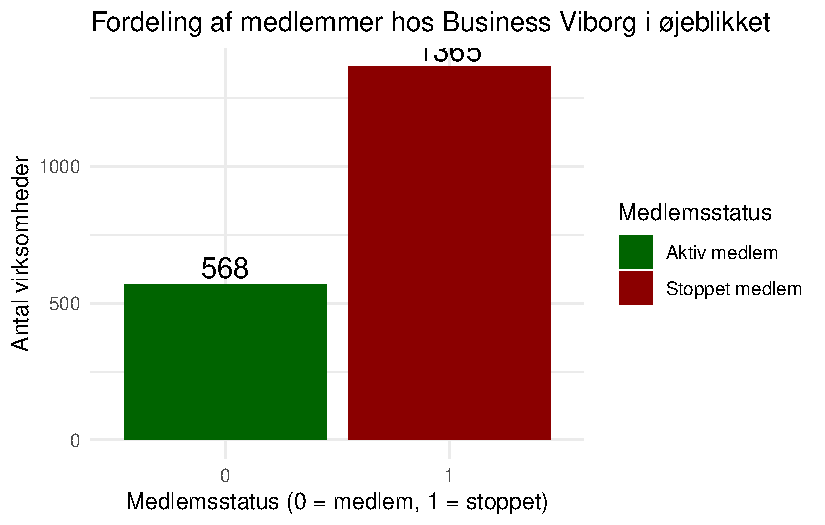
\includegraphics{Quarto_files/figure-pdf/unnamed-chunk-6-1.pdf}

\begin{Shaded}
\begin{Highlighting}[]
\FunctionTok{ggsave}\NormalTok{(}\StringTok{"images/EDA\_1\_fordeling\_medlemmer.png"}\NormalTok{, }\AttributeTok{width =} \DecValTok{7}\NormalTok{, }\AttributeTok{height =} \DecValTok{4}\NormalTok{, }\AttributeTok{dpi =} \DecValTok{300}\NormalTok{)}


\CommentTok{\# 5.2 Søjlediagram: Eventdeltagelse blandt aktive medlemmer}

\CommentTok{\# Visualisering af eventdeltagelse blandt aktive medlemmer}
\CommentTok{\# Her undersøger vi om virksomheder deltager i events, fordelt på \textquotesingle{}Ja\textquotesingle{} og \textquotesingle{}Nej\textquotesingle{}}

\NormalTok{featured }\SpecialCharTok{|\textgreater{}}
  \FunctionTok{filter}\NormalTok{(churn }\SpecialCharTok{==} \DecValTok{0}\NormalTok{) }\SpecialCharTok{|\textgreater{}}
  \FunctionTok{ggplot}\NormalTok{(}\FunctionTok{aes}\NormalTok{(}\AttributeTok{x =}\NormalTok{ deltaget\_i\_event, }\AttributeTok{fill =}\NormalTok{ deltaget\_i\_event)) }\SpecialCharTok{+}
  \FunctionTok{geom\_bar}\NormalTok{() }\SpecialCharTok{+}
  \FunctionTok{geom\_text}\NormalTok{(}\AttributeTok{stat =} \StringTok{"count"}\NormalTok{, }\FunctionTok{aes}\NormalTok{(}\AttributeTok{label =}\NormalTok{ ..count..), }\AttributeTok{vjust =} \SpecialCharTok{{-}}\FloatTok{0.3}\NormalTok{, }\AttributeTok{size =} \DecValTok{5}\NormalTok{) }\SpecialCharTok{+}
  \FunctionTok{scale\_fill\_manual}\NormalTok{(}\AttributeTok{values =} \FunctionTok{c}\NormalTok{(}\StringTok{"Ja"} \OtherTok{=} \StringTok{"darkgreen"}\NormalTok{, }\StringTok{"Nej"} \OtherTok{=} \StringTok{"grey60"}\NormalTok{)) }\SpecialCharTok{+}
  \FunctionTok{labs}\NormalTok{(}
    \AttributeTok{title =} \StringTok{"Eventdeltagelse blandt aktive medlemmer"}\NormalTok{,}
    \AttributeTok{x =} \StringTok{"Deltaget i event?"}\NormalTok{,}
    \AttributeTok{y =} \StringTok{"Antal virksomheder"}\NormalTok{,}
    \AttributeTok{fill =} \StringTok{"Eventdeltagelse"}
\NormalTok{  ) }\SpecialCharTok{+}
  \FunctionTok{theme\_minimal}\NormalTok{()}
\end{Highlighting}
\end{Shaded}

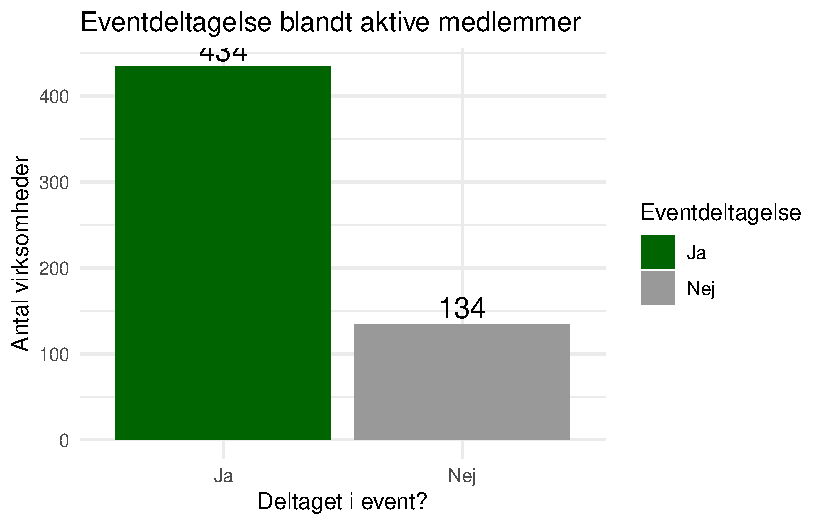
\includegraphics{Quarto_files/figure-pdf/unnamed-chunk-6-2.pdf}

\begin{Shaded}
\begin{Highlighting}[]
\FunctionTok{ggsave}\NormalTok{(}\StringTok{"images/EDA\_2\_eventdeltagelse.png"}\NormalTok{, }\AttributeTok{width =} \DecValTok{7}\NormalTok{, }\AttributeTok{height =} \DecValTok{4}\NormalTok{, }\AttributeTok{dpi =} \DecValTok{300}\NormalTok{)}


\CommentTok{\# 5.3 Søjlediagram: Kombination af kontakt og eventdeltagelse vs. medlemsstatus}


\CommentTok{\# Vi undersøger, hvordan kombinationen af kontakt og eventdeltagelse }
\CommentTok{\# relaterer sig til medlemsstatus (aktiv eller stoppet).}
\CommentTok{\# Derfor opretter vi en ny variabel "kontakt\_event", der grupperer virksomheder}
\CommentTok{\# efter disse kombinationer:}
\CommentTok{\# {-} Både haft kontakt og deltaget i event}
\CommentTok{\# {-} Kun haft kontakt}
\CommentTok{\# {-} Kun deltaget i event}
\CommentTok{\# {-} Ingen af delene}

\NormalTok{featured }\SpecialCharTok{|\textgreater{}} 
  \FunctionTok{mutate}\NormalTok{(}
    \AttributeTok{kontakt\_event =} \FunctionTok{case\_when}\NormalTok{(}
\NormalTok{      har\_haft\_kontakt }\SpecialCharTok{==} \StringTok{"Ja"} \SpecialCharTok{\&}\NormalTok{ deltaget\_i\_event }\SpecialCharTok{==} \StringTok{"Ja"}   \SpecialCharTok{\textasciitilde{}} \StringTok{"Kontakt \& Event"}\NormalTok{,    }
\NormalTok{      har\_haft\_kontakt }\SpecialCharTok{==} \StringTok{"Ja"} \SpecialCharTok{\&}\NormalTok{ deltaget\_i\_event }\SpecialCharTok{==} \StringTok{"Nej"}  \SpecialCharTok{\textasciitilde{}} \StringTok{"Kun kontakt"}\NormalTok{,        }
\NormalTok{      har\_haft\_kontakt }\SpecialCharTok{==} \StringTok{"Nej"} \SpecialCharTok{\&}\NormalTok{ deltaget\_i\_event }\SpecialCharTok{==} \StringTok{"Ja"}  \SpecialCharTok{\textasciitilde{}} \StringTok{"Kun event"}\NormalTok{,          }
      \ConstantTok{TRUE} \SpecialCharTok{\textasciitilde{}} \StringTok{"Ingen af delene"}                                                   
\NormalTok{    )}
\NormalTok{  ) }\SpecialCharTok{|\textgreater{}} 
  \CommentTok{\# Visualiser fordelingen med søjlediagram, hvor vi stabler medlemsstatus (churn)}
  \FunctionTok{ggplot}\NormalTok{(}\FunctionTok{aes}\NormalTok{(}\AttributeTok{x =}\NormalTok{ kontakt\_event, }\AttributeTok{fill =} \FunctionTok{factor}\NormalTok{(churn))) }\SpecialCharTok{+}
  
  \CommentTok{\# geom\_bar tæller antallet af observationer i hver kontakt\_event{-}kategori,}
  \CommentTok{\# og stabler dem efter medlemsstatus (aktiv = 0, stoppet = 1)}
  \FunctionTok{geom\_bar}\NormalTok{(}\AttributeTok{position =} \StringTok{"stack"}\NormalTok{) }\SpecialCharTok{+}
  
  \CommentTok{\# Tilføj antals{-}labels direkte på søjlerne med hvid tekst}
  \FunctionTok{geom\_text}\NormalTok{(}\AttributeTok{stat =} \StringTok{"count"}\NormalTok{, }\FunctionTok{aes}\NormalTok{(}\AttributeTok{label =}\NormalTok{ ..count..),}
            \AttributeTok{position =} \FunctionTok{position\_stack}\NormalTok{(}\AttributeTok{vjust =} \FloatTok{0.5}\NormalTok{), }\AttributeTok{color =} \StringTok{"white"}\NormalTok{, }\AttributeTok{size =} \DecValTok{4}\NormalTok{) }\SpecialCharTok{+}
  
  \CommentTok{\# Definér farver og labels for churn (medlemsstatus)}
  \FunctionTok{scale\_fill\_manual}\NormalTok{(}
    \AttributeTok{values =} \FunctionTok{c}\NormalTok{(}\StringTok{"0"} \OtherTok{=} \StringTok{"darkgreen"}\NormalTok{, }\StringTok{"1"} \OtherTok{=} \StringTok{"darkred"}\NormalTok{),  }\CommentTok{\# Grøn for aktiv, rød for stoppet}
    \AttributeTok{labels =} \FunctionTok{c}\NormalTok{(}\StringTok{"0"} \OtherTok{=} \StringTok{"Aktiv"}\NormalTok{, }\StringTok{"1"} \OtherTok{=} \StringTok{"Stoppet"}\NormalTok{),}
    \AttributeTok{name =} \StringTok{"Medlemsstatus"}
\NormalTok{  ) }\SpecialCharTok{+}
  
  \CommentTok{\# Tilføj titler og akse{-}labels}
  \FunctionTok{labs}\NormalTok{(}
    \AttributeTok{title =} \StringTok{"Kombination af kontakt og eventdeltagelse"}\NormalTok{,}
    \AttributeTok{subtitle =} \StringTok{"Fordelt på medlemsstatus"}\NormalTok{,}
    \AttributeTok{x =} \StringTok{"Kategorier af kontakt og event"}\NormalTok{,}
    \AttributeTok{y =} \StringTok{"Antal virksomheder"}
\NormalTok{  ) }\SpecialCharTok{+}
  
  \CommentTok{\# Brug minimalistisk tema}
  \FunctionTok{theme\_minimal}\NormalTok{() }\SpecialCharTok{+}
  
  \CommentTok{\# Drej x{-}aksens tekst lidt for bedre læsbarhed}
  \FunctionTok{theme}\NormalTok{(}\AttributeTok{axis.text.x =} \FunctionTok{element\_text}\NormalTok{(}\AttributeTok{angle =} \DecValTok{20}\NormalTok{, }\AttributeTok{hjust =} \DecValTok{1}\NormalTok{))}
\end{Highlighting}
\end{Shaded}

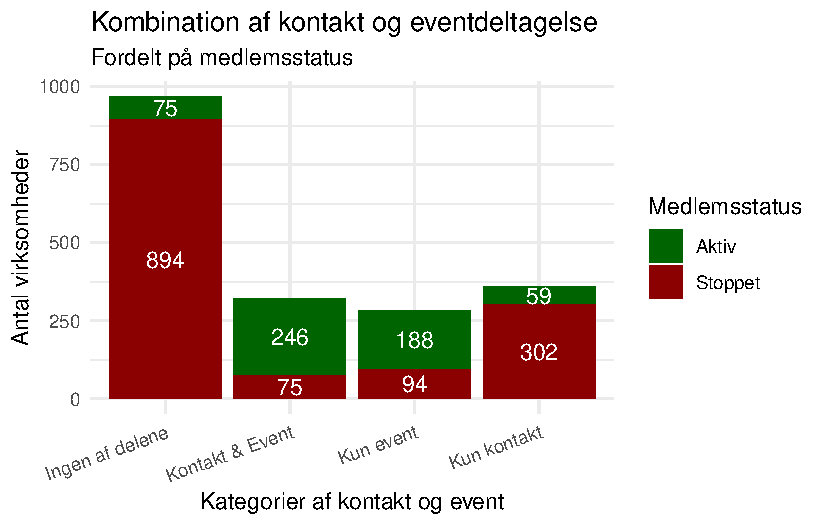
\includegraphics{Quarto_files/figure-pdf/unnamed-chunk-6-3.pdf}

\begin{Shaded}
\begin{Highlighting}[]
\FunctionTok{ggsave}\NormalTok{(}\StringTok{"images/EDA\_3\_kombination\_kontakt\_event.png"}\NormalTok{, }\AttributeTok{width =} \DecValTok{7}\NormalTok{, }\AttributeTok{height =} \DecValTok{4}\NormalTok{, }\AttributeTok{dpi =} \DecValTok{300}\NormalTok{)}

\CommentTok{\# 5.4 Søjlediagram: Branchefordeling blandt aktive medlemmer}


\CommentTok{\# Vi undersøger hvilke brancher de *aktive* virksomheder (medlemmer) tilhører.}
\CommentTok{\# Formålet er at få et overblik over, hvilke brancher der er mest repræsenteret}
\CommentTok{\# blandt dem, der stadig er med i fællesskabet (churn == 0).}
\CommentTok{\# Kun brancher med mindst 10 virksomheder vises, for at sikre et læsbart plot.}

\NormalTok{featured }\SpecialCharTok{|\textgreater{}}
  \CommentTok{\# Filtrér: medtag kun virksomheder der stadig er medlemmer (aktive)}
  \FunctionTok{filter}\NormalTok{(churn }\SpecialCharTok{==} \DecValTok{0}\NormalTok{) }\SpecialCharTok{|\textgreater{}}

  \CommentTok{\# Tæl antallet af virksomheder pr. branche}
  \FunctionTok{count}\NormalTok{(Branche\_navn, }\AttributeTok{name =} \StringTok{"antal"}\NormalTok{) }\SpecialCharTok{|\textgreater{}}

  \CommentTok{\# Fjern brancher med færre end 10 aktive virksomheder}
  \FunctionTok{filter}\NormalTok{(antal }\SpecialCharTok{\textgreater{}=} \DecValTok{10}\NormalTok{) }\SpecialCharTok{|\textgreater{}}

  \CommentTok{\# Sortér brancherne efter antal, så de vises i rigtig rækkefølge i plottet}
  \FunctionTok{mutate}\NormalTok{(}\AttributeTok{Branche\_navn =} \FunctionTok{fct\_reorder}\NormalTok{(Branche\_navn, antal)) }\SpecialCharTok{|\textgreater{}}

  \CommentTok{\# Visualiser fordelingen med søjlediagram}
  \FunctionTok{ggplot}\NormalTok{(}\FunctionTok{aes}\NormalTok{(}\AttributeTok{x =}\NormalTok{ Branche\_navn, }\AttributeTok{y =}\NormalTok{ antal)) }\SpecialCharTok{+}

  \CommentTok{\# geom\_col bruger vores forudberegnede \textquotesingle{}antal\textquotesingle{} til at tegne søjler}
  \FunctionTok{geom\_col}\NormalTok{(}\AttributeTok{fill =} \StringTok{"darkgreen"}\NormalTok{) }\SpecialCharTok{+}

  \CommentTok{\# Tilføj antals{-}labels til søjlerne (antal virksomheder)}
  \FunctionTok{geom\_text}\NormalTok{(}\FunctionTok{aes}\NormalTok{(}\AttributeTok{label =}\NormalTok{ antal), }\AttributeTok{hjust =} \SpecialCharTok{{-}}\FloatTok{0.1}\NormalTok{, }\AttributeTok{size =} \DecValTok{4}\NormalTok{) }\SpecialCharTok{+}

  \CommentTok{\# Vend koordinaterne, så brancherne vises lodret og er nemmere at læse}
  \FunctionTok{coord\_flip}\NormalTok{() }\SpecialCharTok{+}

  \CommentTok{\# Tilføj titel, undertitel og aksetekster}
  \FunctionTok{labs}\NormalTok{(}
    \AttributeTok{title =} \StringTok{"Branchefordeling blandt aktive medlemmer"}\NormalTok{,}
    \AttributeTok{subtitle =} \StringTok{"Viser kun brancher med mindst 10 aktive virksomheder"}\NormalTok{,}
    \AttributeTok{x =} \StringTok{"Branche"}\NormalTok{,}
    \AttributeTok{y =} \StringTok{"Antal virksomheder"}
\NormalTok{  ) }\SpecialCharTok{+}

  \CommentTok{\# Brug minimalistisk tema for et rent visuelt udtryk}
  \FunctionTok{theme\_minimal}\NormalTok{()}
\end{Highlighting}
\end{Shaded}

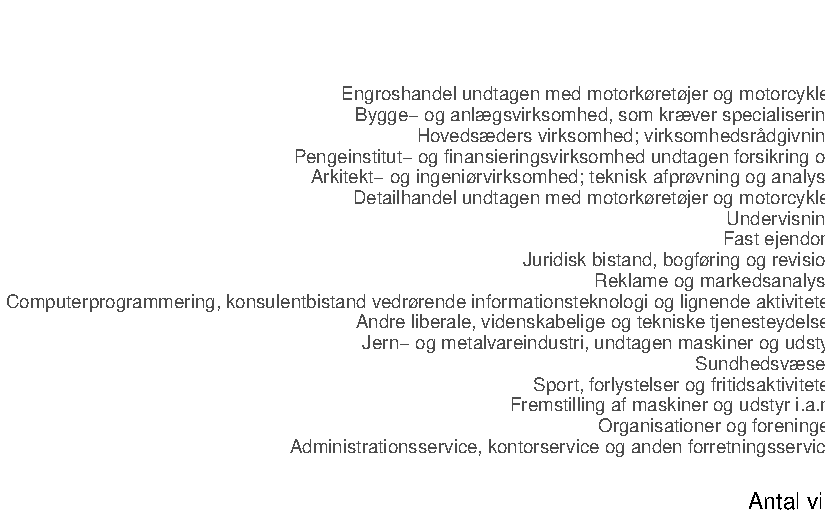
\includegraphics{Quarto_files/figure-pdf/unnamed-chunk-6-4.pdf}

\begin{Shaded}
\begin{Highlighting}[]
\FunctionTok{ggsave}\NormalTok{(}\StringTok{"images/EDA\_4\_branchefordeling.png"}\NormalTok{, }\AttributeTok{width =} \DecValTok{7}\NormalTok{, }\AttributeTok{height =} \DecValTok{4}\NormalTok{, }\AttributeTok{dpi =} \DecValTok{300}\NormalTok{)}


\CommentTok{\# 5.5 Søjlediagram: Eventdeltagelse pr. postnummer (Aktive medlemmer)}


\CommentTok{\# Vi undersøger, hvordan aktive virksomheders eventdeltagelse fordeler sig geografisk,}
\CommentTok{\# baseret på postnummer. Vi viser både deltagelse ("Ja") og ikke{-}deltagelse ("Nej"),}
\CommentTok{\# og sorterer postnumrene efter hvor stor andelen af \textquotesingle{}Ja\textquotesingle{}{-}svar er.}

\CommentTok{\# Beregn antal og andel for hver kombination af postnummer og eventdeltagelse}
\NormalTok{post\_event }\OtherTok{\textless{}{-}}\NormalTok{ featured }\SpecialCharTok{|\textgreater{}} 
  \CommentTok{\# Filtrér: medtag kun aktive virksomheder}
  \FunctionTok{filter}\NormalTok{(churn }\SpecialCharTok{==} \DecValTok{0}\NormalTok{) }\SpecialCharTok{|\textgreater{}} 
  
  \CommentTok{\# Tæl antallet af virksomheder pr. postnummer og eventstatus}
  \FunctionTok{count}\NormalTok{(PostalCode, deltaget\_i\_event, }\AttributeTok{name =} \StringTok{"antal"}\NormalTok{) }\SpecialCharTok{|\textgreater{}} 
  
  \CommentTok{\# Beregn total antal og procentuel andel inden for hvert postnummer}
  \FunctionTok{group\_by}\NormalTok{(PostalCode) }\SpecialCharTok{|\textgreater{}} 
  \FunctionTok{mutate}\NormalTok{(}
    \AttributeTok{total =} \FunctionTok{sum}\NormalTok{(antal),                              }\CommentTok{\# Total antal virksomheder}
    \AttributeTok{andel =} \FunctionTok{round}\NormalTok{(antal }\SpecialCharTok{/}\NormalTok{ total }\SpecialCharTok{*} \DecValTok{100}\NormalTok{, }\DecValTok{1}\NormalTok{)            }\CommentTok{\# Andel i procent}
\NormalTok{  ) }\SpecialCharTok{|\textgreater{}} 
  \FunctionTok{ungroup}\NormalTok{()}

\CommentTok{\# Sortér postnumre efter andel af virksomheder der har deltaget i events ("Ja")}
\NormalTok{post\_order }\OtherTok{\textless{}{-}}\NormalTok{ post\_event }\SpecialCharTok{|\textgreater{}} 
  \FunctionTok{filter}\NormalTok{(deltaget\_i\_event }\SpecialCharTok{==} \StringTok{"Ja"}\NormalTok{) }\SpecialCharTok{|\textgreater{}} 
  \FunctionTok{arrange}\NormalTok{(}\FunctionTok{desc}\NormalTok{(andel)) }\SpecialCharTok{|\textgreater{}} 
  \FunctionTok{pull}\NormalTok{(PostalCode)}

\CommentTok{\# Visualiser data som stacked søjlediagram}
\NormalTok{post\_event }\SpecialCharTok{|\textgreater{}} 
  \CommentTok{\# Sortér postnumrene i plottet efter andel \textquotesingle{}Ja\textquotesingle{}}
  \FunctionTok{mutate}\NormalTok{(}\AttributeTok{PostalCode =} \FunctionTok{factor}\NormalTok{(PostalCode, }\AttributeTok{levels =}\NormalTok{ post\_order)) }\SpecialCharTok{|\textgreater{}} 
  
  \CommentTok{\# Opret plot med antal virksomheder pr. postnummer, farvet efter eventdeltagelse}
  \FunctionTok{ggplot}\NormalTok{(}\FunctionTok{aes}\NormalTok{(}\AttributeTok{x =}\NormalTok{ PostalCode, }\AttributeTok{y =}\NormalTok{ antal, }\AttributeTok{fill =}\NormalTok{ deltaget\_i\_event)) }\SpecialCharTok{+}
  
  \CommentTok{\# geom\_col tegner stablede søjler}
  \FunctionTok{geom\_col}\NormalTok{() }\SpecialCharTok{+}
  
  \CommentTok{\# Tilføj antalslabels midt i søjlerne}
  \FunctionTok{geom\_text}\NormalTok{(}\FunctionTok{aes}\NormalTok{(}\AttributeTok{label =}\NormalTok{ antal), }\AttributeTok{position =} \FunctionTok{position\_stack}\NormalTok{(}\AttributeTok{vjust =} \FloatTok{0.5}\NormalTok{), }
            \AttributeTok{color =} \StringTok{"white"}\NormalTok{, }\AttributeTok{size =} \FloatTok{3.5}\NormalTok{) }\SpecialCharTok{+}
  
  \CommentTok{\# Brug manuelle farver: grøn = deltager, grå = deltager ikke}
  \FunctionTok{scale\_fill\_manual}\NormalTok{(}\AttributeTok{values =} \FunctionTok{c}\NormalTok{(}\StringTok{"Ja"} \OtherTok{=} \StringTok{"darkgreen"}\NormalTok{, }\StringTok{"Nej"} \OtherTok{=} \StringTok{"grey60"}\NormalTok{)) }\SpecialCharTok{+}
  
  \CommentTok{\# Vend koordinatsystemet for bedre læsbarhed}
  \FunctionTok{coord\_flip}\NormalTok{() }\SpecialCharTok{+}
  
  \CommentTok{\# Tilføj titel, aksetitler og farveforklaring}
  \FunctionTok{labs}\NormalTok{(}
    \AttributeTok{title =} \StringTok{"Eventdeltagelse pr. postnummer (aktive virksomheder)"}\NormalTok{,}
    \AttributeTok{subtitle =} \StringTok{"Sorteret efter postnumre med flest \textquotesingle{}Ja\textquotesingle{}{-}svar"}\NormalTok{,}
    \AttributeTok{x =} \StringTok{"Postnummer"}\NormalTok{,}
    \AttributeTok{y =} \StringTok{"Antal virksomheder"}\NormalTok{,}
    \AttributeTok{fill =} \StringTok{"Eventdeltagelse"}
\NormalTok{  ) }\SpecialCharTok{+}
  
  \CommentTok{\# Brug minimalistisk ggplot{-}tema}
  \FunctionTok{theme\_minimal}\NormalTok{()}
\end{Highlighting}
\end{Shaded}

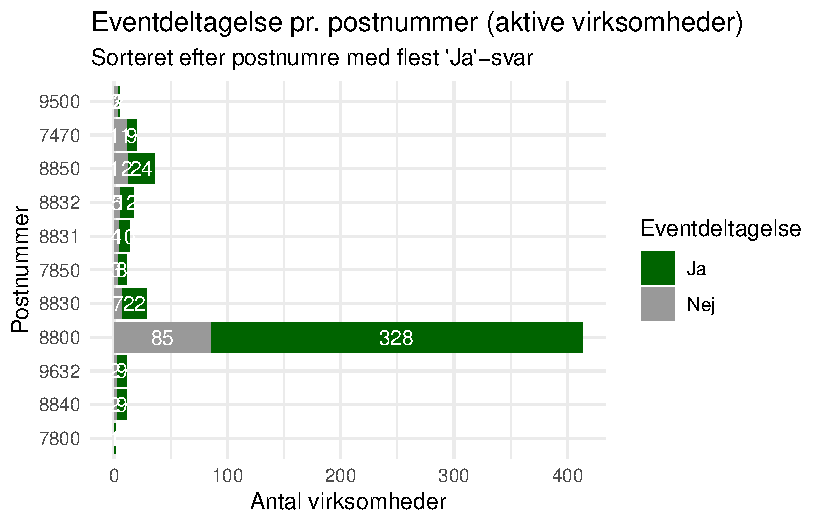
\includegraphics{Quarto_files/figure-pdf/unnamed-chunk-6-5.pdf}

\begin{Shaded}
\begin{Highlighting}[]
\FunctionTok{ggsave}\NormalTok{(}\StringTok{"images/EDA\_5\_eventdeltagelse\_postnummer.png"}\NormalTok{, }\AttributeTok{width =} \DecValTok{7}\NormalTok{, }\AttributeTok{height =} \DecValTok{4}\NormalTok{, }\AttributeTok{dpi =} \DecValTok{300}\NormalTok{)}

\CommentTok{\# 5.6 Korrellationsmatrix: Numeriske variable}

\CommentTok{\# Vi ønsker at undersøge, hvordan de numeriske variable i datasættet hænger sammen.}
\CommentTok{\# Det gør vi ved at udtrække alle numeriske kolonner og beregne en korrelationsmatrix.}
\CommentTok{\# Denne visualiseres som et cirkelplot med Pearson{-}korrelationer.}

\CommentTok{\# Udtræk kun de kolonner i datasættet, der er numeriske}
\NormalTok{featured\_numerisk }\OtherTok{\textless{}{-}}\NormalTok{ featured }\SpecialCharTok{|\textgreater{}} 
  \FunctionTok{select}\NormalTok{(}\FunctionTok{where}\NormalTok{(is.numeric)) }\SpecialCharTok{|\textgreater{}} 
  
  \CommentTok{\# Fjern rækker med NA{-}værdier, da korrelationsberegning kræver komplette værdier}
  \FunctionTok{drop\_na}\NormalTok{()}

\CommentTok{\# Beregn korrelationsmatrix ved hjælp af Pearson\textquotesingle{}s metode}
\NormalTok{cor\_matrix }\OtherTok{\textless{}{-}} \FunctionTok{cor}\NormalTok{(featured\_numerisk, }\AttributeTok{use =} \StringTok{"pairwise.complete.obs"}\NormalTok{)}

\CommentTok{\# Afrund korrelationerne til 2 decimaler for pænere visning (valgfrit trin)}
\NormalTok{cor\_matrix\_rounded }\OtherTok{\textless{}{-}} \FunctionTok{round}\NormalTok{(cor\_matrix, }\DecValTok{2}\NormalTok{)}

\CommentTok{\# Visualisér korrelationerne med et "cirkelplot" fra pakken \textquotesingle{}corrplot\textquotesingle{}}
\NormalTok{corrplot}\SpecialCharTok{::}\FunctionTok{corrplot}\NormalTok{(}
\NormalTok{  cor\_matrix,}
  
  \AttributeTok{method =} \StringTok{"circle"}\NormalTok{,       }\CommentTok{\# Brug cirkler til at vise styrke og retning af korrelation}
  \AttributeTok{type =} \StringTok{"lower"}\NormalTok{,          }\CommentTok{\# Vis kun nederste trekant (mere overskueligt)}
  
  \CommentTok{\# Tekst og talindstillinger}
  \AttributeTok{tl.cex =} \FloatTok{0.8}\NormalTok{,            }\CommentTok{\# Størrelse på tekstetiketter (variabelnavne)}
  \AttributeTok{tl.col =} \StringTok{"black"}\NormalTok{,        }\CommentTok{\# Farve på variabelnavne}
  
  \AttributeTok{addCoef.col =} \StringTok{"darkgreen"}    \CommentTok{\# Vis selve korrelationstallet inde i cirklerne}
\NormalTok{)}
\end{Highlighting}
\end{Shaded}

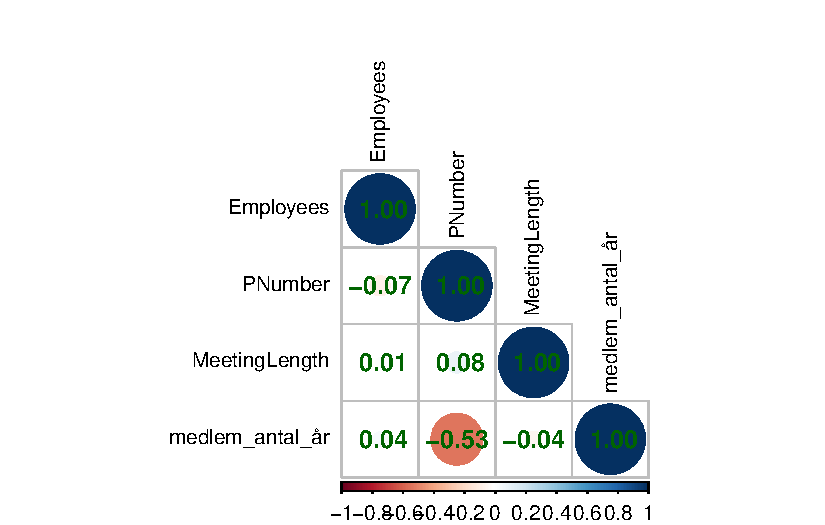
\includegraphics{Quarto_files/figure-pdf/unnamed-chunk-6-6.pdf}

\begin{Shaded}
\begin{Highlighting}[]
\CommentTok{\#ggsave("images/EDA\_6\_korrellationsmatrix.png", width = 7, height = 4, dpi = 300)}


\CommentTok{\# 5.7 Boxplot: Mødelængde vs. eventdeltagelse (kun aktive medlemmer)}

\CommentTok{\# Outlier{-}funktion med IQR{-}metoden}
\NormalTok{find\_outliers }\OtherTok{\textless{}{-}} \ControlFlowTok{function}\NormalTok{(x) \{}
\NormalTok{  iqr }\OtherTok{\textless{}{-}} \FunctionTok{IQR}\NormalTok{(x, }\AttributeTok{na.rm =} \ConstantTok{TRUE}\NormalTok{)}
\NormalTok{  lower }\OtherTok{\textless{}{-}} \FunctionTok{quantile}\NormalTok{(x, }\FloatTok{0.25}\NormalTok{, }\AttributeTok{na.rm =} \ConstantTok{TRUE}\NormalTok{) }\SpecialCharTok{{-}} \FloatTok{1.5} \SpecialCharTok{*}\NormalTok{ iqr}
\NormalTok{  upper }\OtherTok{\textless{}{-}} \FunctionTok{quantile}\NormalTok{(x, }\FloatTok{0.75}\NormalTok{, }\AttributeTok{na.rm =} \ConstantTok{TRUE}\NormalTok{) }\SpecialCharTok{+} \FloatTok{1.5} \SpecialCharTok{*}\NormalTok{ iqr}
\NormalTok{  x }\SpecialCharTok{\textless{}}\NormalTok{ lower }\SpecialCharTok{|}\NormalTok{ x }\SpecialCharTok{\textgreater{}}\NormalTok{ upper}
\NormalTok{\}}

\CommentTok{\# Gør datasættet klar: filtrér aktive, identificér outliers og opret grupper}
\NormalTok{meeting\_event }\OtherTok{\textless{}{-}}\NormalTok{ featured }\SpecialCharTok{|\textgreater{}} 
  \FunctionTok{filter}\NormalTok{(churn }\SpecialCharTok{==} \DecValTok{0}\NormalTok{, }\SpecialCharTok{!}\FunctionTok{is.na}\NormalTok{(MeetingLength)) }\SpecialCharTok{|\textgreater{}} 
  \FunctionTok{mutate}\NormalTok{(}
    \AttributeTok{Eventgruppe =} \FunctionTok{fct\_relevel}\NormalTok{(}
      \FunctionTok{if\_else}\NormalTok{(deltaget\_i\_event }\SpecialCharTok{==} \StringTok{"Ja"}\NormalTok{, }\StringTok{"Deltager i event"}\NormalTok{, }\StringTok{"Deltager ikke"}\NormalTok{),}
      \StringTok{"Deltager i event"}\NormalTok{, }\StringTok{"Deltager ikke"}
\NormalTok{    ),}
    \AttributeTok{outlier =} \FunctionTok{find\_outliers}\NormalTok{(MeetingLength)}
\NormalTok{  )}

\CommentTok{\# Statistik til annotationer}
\NormalTok{meeting\_stats }\OtherTok{\textless{}{-}}\NormalTok{ meeting\_event }\SpecialCharTok{|\textgreater{}} 
  \FunctionTok{group\_by}\NormalTok{(Eventgruppe) }\SpecialCharTok{|\textgreater{}} 
  \FunctionTok{summarise}\NormalTok{(}
    \AttributeTok{antal =} \FunctionTok{n}\NormalTok{(),}
    \AttributeTok{gennemsnit =} \FunctionTok{round}\NormalTok{(}\FunctionTok{mean}\NormalTok{(MeetingLength), }\DecValTok{1}\NormalTok{),}
    \AttributeTok{outliers =} \FunctionTok{sum}\NormalTok{(outlier),}
    \AttributeTok{.groups =} \StringTok{"drop"}
\NormalTok{  )}

\CommentTok{\# Brug max{-}værdi til annotation}
\NormalTok{max\_y }\OtherTok{\textless{}{-}} \FunctionTok{max}\NormalTok{(meeting\_event}\SpecialCharTok{$}\NormalTok{MeetingLength, }\AttributeTok{na.rm =} \ConstantTok{TRUE}\NormalTok{) }\SpecialCharTok{+} \DecValTok{5}

\CommentTok{\# Visualisering}
\NormalTok{meeting\_event }\SpecialCharTok{|\textgreater{}} 
  \FunctionTok{ggplot}\NormalTok{(}\FunctionTok{aes}\NormalTok{(}\AttributeTok{x =}\NormalTok{ Eventgruppe, }\AttributeTok{y =}\NormalTok{ MeetingLength, }\AttributeTok{fill =}\NormalTok{ Eventgruppe)) }\SpecialCharTok{+}
  
  \CommentTok{\# Boxplot uden standard outliers}
  \FunctionTok{geom\_boxplot}\NormalTok{(}\AttributeTok{alpha =} \FloatTok{0.7}\NormalTok{, }\AttributeTok{outlier.shape =} \ConstantTok{NA}\NormalTok{) }\SpecialCharTok{+}

  \CommentTok{\# Manuelle outliers med jitter}
  \FunctionTok{geom\_point}\NormalTok{(}\AttributeTok{data =} \FunctionTok{filter}\NormalTok{(meeting\_event, outlier),}
             \FunctionTok{aes}\NormalTok{(}\AttributeTok{x =}\NormalTok{ Eventgruppe, }\AttributeTok{y =}\NormalTok{ MeetingLength),}
             \AttributeTok{color =} \StringTok{"blue"}\NormalTok{, }\AttributeTok{alpha =} \FloatTok{0.6}\NormalTok{, }\AttributeTok{size =} \DecValTok{2}\NormalTok{,}
             \AttributeTok{position =} \FunctionTok{position\_jitter}\NormalTok{(}\AttributeTok{width =} \FloatTok{0.2}\NormalTok{)) }\SpecialCharTok{+}
  
  \CommentTok{\# Rød prik for gennemsnit}
  \FunctionTok{stat\_summary}\NormalTok{(}\AttributeTok{fun =}\NormalTok{ mean, }\AttributeTok{geom =} \StringTok{"point"}\NormalTok{, }\AttributeTok{shape =} \DecValTok{18}\NormalTok{, }\AttributeTok{size =} \DecValTok{3}\NormalTok{, }
               \AttributeTok{color =} \StringTok{"darkred"}\NormalTok{) }\SpecialCharTok{+}
  
  \CommentTok{\# Annotér antal pr. gruppe}
  \FunctionTok{geom\_text}\NormalTok{(}\AttributeTok{data =}\NormalTok{ meeting\_stats, }\FunctionTok{aes}\NormalTok{(}\AttributeTok{x =}\NormalTok{ Eventgruppe, }\AttributeTok{y =}\NormalTok{ max\_y,}
                                      \AttributeTok{label =} \FunctionTok{paste0}\NormalTok{(}\StringTok{"n = "}\NormalTok{, antal)),}
            \AttributeTok{size =} \DecValTok{4}\NormalTok{) }\SpecialCharTok{+}
  
  \CommentTok{\# Annotér gennemsnit}
  \FunctionTok{geom\_text}\NormalTok{(}\AttributeTok{data =}\NormalTok{ meeting\_stats, }\FunctionTok{aes}\NormalTok{(}\AttributeTok{x =}\NormalTok{ Eventgruppe, }\AttributeTok{y =}\NormalTok{ gennemsnit,}
                                      \AttributeTok{label =} \FunctionTok{paste0}\NormalTok{(}\StringTok{"Gns: "}\NormalTok{, gennemsnit, }
                                                     \StringTok{" min"}\NormalTok{)),}
            \AttributeTok{size =} \DecValTok{4}\NormalTok{, }\AttributeTok{color =} \StringTok{"darkred"}\NormalTok{, }\AttributeTok{nudge\_y =} \DecValTok{5}\NormalTok{) }\SpecialCharTok{+}
  
  \CommentTok{\# Vend akser}
  \FunctionTok{coord\_flip}\NormalTok{() }\SpecialCharTok{+}
  
  \CommentTok{\# Farver}
  \FunctionTok{scale\_fill\_manual}\NormalTok{(}\AttributeTok{values =} \FunctionTok{c}\NormalTok{(}\StringTok{"Deltager i event"} \OtherTok{=} \StringTok{"darkgreen"}\NormalTok{, }
                               \StringTok{"Deltager ikke"} \OtherTok{=} \StringTok{"red"}\NormalTok{)) }\SpecialCharTok{+}
  
  \CommentTok{\# Titler og akser}
  \FunctionTok{labs}\NormalTok{(}
    \AttributeTok{title =} \StringTok{"Mødelængde vs. eventdeltagelse (aktive medlemmer)"}\NormalTok{,}
    \AttributeTok{subtitle =} \StringTok{"Rød prik = gennemsnit • Blå prikker = outliers"}\NormalTok{,}
    \AttributeTok{x =} \ConstantTok{NULL}\NormalTok{,}
    \AttributeTok{y =} \StringTok{"Mødelængde (minutter)"}
\NormalTok{  ) }\SpecialCharTok{+}
  
  \CommentTok{\# Tema og layoutjusteringer}
  \FunctionTok{theme\_minimal}\NormalTok{(}\AttributeTok{base\_size =} \DecValTok{13}\NormalTok{) }\SpecialCharTok{+}
  \FunctionTok{theme}\NormalTok{(}
  \AttributeTok{legend.position =} \StringTok{"none"}\NormalTok{,}
  \AttributeTok{plot.title =} \FunctionTok{element\_text}\NormalTok{(}\AttributeTok{face =} \StringTok{"bold"}\NormalTok{),}
  \AttributeTok{plot.subtitle =} \FunctionTok{element\_text}\NormalTok{(}\AttributeTok{margin =} \FunctionTok{unit}\NormalTok{(}\FunctionTok{c}\NormalTok{(}\DecValTok{0}\NormalTok{, }\DecValTok{0}\NormalTok{, }\DecValTok{10}\NormalTok{, }\DecValTok{0}\NormalTok{), }\StringTok{"pt"}\NormalTok{)),}
  \AttributeTok{axis.title.y =} \FunctionTok{element\_text}\NormalTok{(}\AttributeTok{margin =} \FunctionTok{unit}\NormalTok{(}\FunctionTok{c}\NormalTok{(}\DecValTok{0}\NormalTok{, }\DecValTok{10}\NormalTok{, }\DecValTok{0}\NormalTok{, }\DecValTok{0}\NormalTok{), }\StringTok{"pt"}\NormalTok{))}
\NormalTok{  )}
\end{Highlighting}
\end{Shaded}

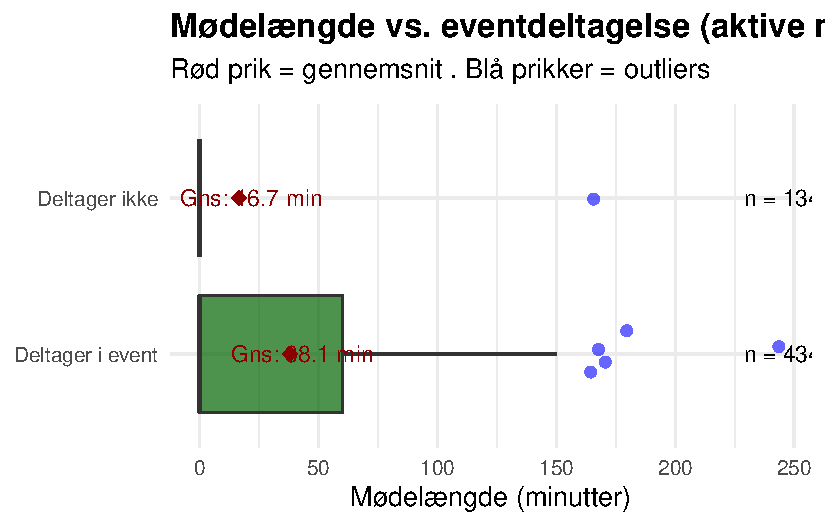
\includegraphics{Quarto_files/figure-pdf/unnamed-chunk-6-7.pdf}

\begin{Shaded}
\begin{Highlighting}[]
\FunctionTok{ggsave}\NormalTok{(}\StringTok{"images/EDA\_7\_mødelængde\_eventdeltagelse.png"}\NormalTok{, }\AttributeTok{width =} \DecValTok{7}\NormalTok{, }\AttributeTok{height =} \DecValTok{4}\NormalTok{, }
       \AttributeTok{dpi =} \DecValTok{300}\NormalTok{)}
\end{Highlighting}
\end{Shaded}

\begin{Shaded}
\begin{Highlighting}[]
\CommentTok{\# {-}{-}{-}{-}{-}{-}{-}{-}{-}{-}{-}{-}{-}{-}{-}{-}{-}{-}{-}{-}{-}{-}{-}{-}{-}{-}{-}{-}{-}{-}{-}{-}{-}{-}{-}{-}{-}{-}{-}{-}{-}{-}{-}{-}{-}{-}{-}{-}{-}{-}{-}{-}{-}{-}{-}{-}{-}{-}{-}{-}{-}{-}{-}{-}{-}{-}{-}{-}{-}{-}{-}{-}{-}{-}{-}{-}{-}{-}}
\CommentTok{\# 6. Preprocessing}
\CommentTok{\# {-}{-}{-}{-}{-}{-}{-}{-}{-}{-}{-}{-}{-}{-}{-}{-}{-}{-}{-}{-}{-}{-}{-}{-}{-}{-}{-}{-}{-}{-}{-}{-}{-}{-}{-}{-}{-}{-}{-}{-}{-}{-}{-}{-}{-}{-}{-}{-}{-}{-}{-}{-}{-}{-}{-}{-}{-}{-}{-}{-}{-}{-}{-}{-}{-}{-}{-}{-}{-}{-}{-}{-}{-}{-}{-}{-}{-}{-}}
\FunctionTok{set.seed}\NormalTok{(}\DecValTok{2025}\NormalTok{)}

\NormalTok{churn\_split }\OtherTok{\textless{}{-}} \FunctionTok{initial\_split}\NormalTok{(feature\_engineering, }\AttributeTok{prop =} \FloatTok{0.8}\NormalTok{, }\AttributeTok{strata =}\NormalTok{ churn)}
\NormalTok{churn\_train }\OtherTok{\textless{}{-}} \FunctionTok{training}\NormalTok{(churn\_split)}
\NormalTok{churn\_test  }\OtherTok{\textless{}{-}} \FunctionTok{testing}\NormalTok{(churn\_split)}

\NormalTok{churn\_folds }\OtherTok{\textless{}{-}} \FunctionTok{vfold\_cv}\NormalTok{(churn\_train, }\AttributeTok{v =} \DecValTok{10}\NormalTok{, }\AttributeTok{strata =}\NormalTok{ churn)}

\NormalTok{churn\_recipe }\OtherTok{\textless{}{-}} 
  \FunctionTok{recipe}\NormalTok{(churn }\SpecialCharTok{\textasciitilde{}}\NormalTok{ ., }\AttributeTok{data =}\NormalTok{ churn\_train) }\SpecialCharTok{|\textgreater{}}
  \FunctionTok{update\_role}\NormalTok{(PNumber, }\AttributeTok{new\_role =} \StringTok{"ID"}\NormalTok{) }\SpecialCharTok{|\textgreater{}}  \CommentTok{\# PNumber bevares, men bruges ikke som predictor}
  \FunctionTok{step\_novel}\NormalTok{(}\FunctionTok{all\_nominal\_predictors}\NormalTok{()) }\SpecialCharTok{|\textgreater{}} 
  \FunctionTok{step\_dummy}\NormalTok{(}\FunctionTok{all\_nominal\_predictors}\NormalTok{(), }\AttributeTok{one\_hot =} \ConstantTok{TRUE}\NormalTok{) }\SpecialCharTok{|\textgreater{}}
  \FunctionTok{step\_zv}\NormalTok{(}\FunctionTok{all\_predictors}\NormalTok{()) }\SpecialCharTok{|\textgreater{}} 
  \FunctionTok{step\_normalize}\NormalTok{(}\FunctionTok{all\_numeric\_predictors}\NormalTok{()) }\SpecialCharTok{|\textgreater{}} 
  \FunctionTok{step\_downsample}\NormalTok{(churn)  }\CommentTok{\# Brug evt. step\_smote(churn) hvis ekstrem ubalance}
\end{Highlighting}
\end{Shaded}

\begin{Shaded}
\begin{Highlighting}[]
\CommentTok{\# {-}{-}{-}{-}{-}{-}{-}{-}{-}{-}{-}{-}{-}{-}{-}{-}{-}{-}{-}{-}{-}{-}{-}{-}{-}{-}{-}{-}{-}{-}{-}{-}{-}{-}{-}{-}{-}{-}{-}{-}{-}{-}{-}{-}{-}{-}{-}{-}{-}{-}{-}{-}{-}{-}{-}{-}{-}{-}{-}{-}{-}{-}{-}{-}{-}{-}{-}{-}{-}{-}{-}{-}{-}{-}{-}{-}{-}{-}}
\CommentTok{\# 7. Modelling}
\CommentTok{\# {-}{-}{-}{-}{-}{-}{-}{-}{-}{-}{-}{-}{-}{-}{-}{-}{-}{-}{-}{-}{-}{-}{-}{-}{-}{-}{-}{-}{-}{-}{-}{-}{-}{-}{-}{-}{-}{-}{-}{-}{-}{-}{-}{-}{-}{-}{-}{-}{-}{-}{-}{-}{-}{-}{-}{-}{-}{-}{-}{-}{-}{-}{-}{-}{-}{-}{-}{-}{-}{-}{-}{-}{-}{-}{-}{-}{-}{-}}

\CommentTok{\# Model specs}
\NormalTok{rf\_spec }\OtherTok{\textless{}{-}} \FunctionTok{rand\_forest}\NormalTok{(}\AttributeTok{mtry =} \FunctionTok{tune}\NormalTok{(), }\AttributeTok{min\_n =} \FunctionTok{tune}\NormalTok{()) }\SpecialCharTok{|\textgreater{}}
  \FunctionTok{set\_engine}\NormalTok{(}\StringTok{"ranger"}\NormalTok{, }\AttributeTok{importance =} \StringTok{"impurity"}\NormalTok{) }\SpecialCharTok{|\textgreater{}}
  \FunctionTok{set\_mode}\NormalTok{(}\StringTok{"classification"}\NormalTok{)}

\NormalTok{xgb\_spec }\OtherTok{\textless{}{-}} \FunctionTok{boost\_tree}\NormalTok{(}\AttributeTok{trees =} \FunctionTok{tune}\NormalTok{(), }\AttributeTok{mtry =} \FunctionTok{tune}\NormalTok{(), }\AttributeTok{learn\_rate =} \FunctionTok{tune}\NormalTok{()) }\SpecialCharTok{|\textgreater{}}
  \FunctionTok{set\_engine}\NormalTok{(}\StringTok{"xgboost"}\NormalTok{) }\SpecialCharTok{|\textgreater{}}
  \FunctionTok{set\_mode}\NormalTok{(}\StringTok{"classification"}\NormalTok{)}

\NormalTok{log\_reg\_spec }\OtherTok{\textless{}{-}} \FunctionTok{logistic\_reg}\NormalTok{(}\AttributeTok{penalty =} \FunctionTok{tune}\NormalTok{(), }\AttributeTok{mixture =} \FunctionTok{tune}\NormalTok{()) }\SpecialCharTok{|\textgreater{}}
  \FunctionTok{set\_engine}\NormalTok{(}\StringTok{"glmnet"}\NormalTok{) }\SpecialCharTok{|\textgreater{}}
  \FunctionTok{set\_mode}\NormalTok{(}\StringTok{"classification"}\NormalTok{)}

\NormalTok{knn\_spec }\OtherTok{\textless{}{-}} \FunctionTok{nearest\_neighbor}\NormalTok{(}\AttributeTok{neighbors =} \FunctionTok{tune}\NormalTok{(), }\AttributeTok{weight\_func =} \FunctionTok{tune}\NormalTok{()) }\SpecialCharTok{|\textgreater{}}
  \FunctionTok{set\_engine}\NormalTok{(}\StringTok{"kknn"}\NormalTok{) }\SpecialCharTok{|\textgreater{}}
  \FunctionTok{set\_mode}\NormalTok{(}\StringTok{"classification"}\NormalTok{)}

\NormalTok{nb\_spec }\OtherTok{\textless{}{-}} \FunctionTok{naive\_Bayes}\NormalTok{(}\AttributeTok{smoothness =} \FunctionTok{tune}\NormalTok{(), }\AttributeTok{Laplace =} \FunctionTok{tune}\NormalTok{()) }\SpecialCharTok{|\textgreater{}}
  \FunctionTok{set\_engine}\NormalTok{(}\StringTok{"naivebayes"}\NormalTok{) }\SpecialCharTok{|\textgreater{}}
  \FunctionTok{set\_mode}\NormalTok{(}\StringTok{"classification"}\NormalTok{)}

\NormalTok{svm\_spec }\OtherTok{\textless{}{-}} \FunctionTok{svm\_rbf}\NormalTok{(}\AttributeTok{cost =} \FunctionTok{tune}\NormalTok{(), }\AttributeTok{rbf\_sigma =} \FunctionTok{tune}\NormalTok{()) }\SpecialCharTok{|\textgreater{}}
  \FunctionTok{set\_engine}\NormalTok{(}\StringTok{"kernlab"}\NormalTok{) }\SpecialCharTok{|\textgreater{}}
  \FunctionTok{set\_mode}\NormalTok{(}\StringTok{"classification"}\NormalTok{)}

\CommentTok{\# Samlet workflow set}
\NormalTok{churn\_workflow\_set }\OtherTok{\textless{}{-}} \FunctionTok{workflow\_set}\NormalTok{(}
  \AttributeTok{preproc =} \FunctionTok{list}\NormalTok{(}\AttributeTok{churn\_recipe =}\NormalTok{ churn\_recipe),}
  \AttributeTok{models =} \FunctionTok{list}\NormalTok{(}
    \AttributeTok{rf =}\NormalTok{ rf\_spec,}
    \AttributeTok{xgboost =}\NormalTok{ xgb\_spec,}
    \AttributeTok{logistic =}\NormalTok{ log\_reg\_spec,}
    \AttributeTok{knn =}\NormalTok{ knn\_spec,}
    \AttributeTok{naive\_bayes =}\NormalTok{ nb\_spec,}
    \AttributeTok{svm\_rbf =}\NormalTok{ svm\_spec}
\NormalTok{  )}
\NormalTok{)}
\end{Highlighting}
\end{Shaded}

\begin{Shaded}
\begin{Highlighting}[]
\CommentTok{\# {-}{-}{-}{-}{-}{-}{-}{-}{-}{-}{-}{-}{-}{-}{-}{-}{-}{-}{-}{-}{-}{-}{-}{-}{-}{-}{-}{-}{-}{-}{-}{-}{-}{-}{-}{-}{-}{-}{-}{-}{-}{-}{-}{-}{-}{-}{-}{-}{-}{-}{-}{-}{-}{-}{-}{-}{-}{-}{-}{-}{-}{-}{-}{-}{-}{-}{-}{-}{-}{-}{-}{-}{-}{-}{-}{-}{-}{-}}
\CommentTok{\# 8. Evaluate metrics}
\CommentTok{\# {-}{-}{-}{-}{-}{-}{-}{-}{-}{-}{-}{-}{-}{-}{-}{-}{-}{-}{-}{-}{-}{-}{-}{-}{-}{-}{-}{-}{-}{-}{-}{-}{-}{-}{-}{-}{-}{-}{-}{-}{-}{-}{-}{-}{-}{-}{-}{-}{-}{-}{-}{-}{-}{-}{-}{-}{-}{-}{-}{-}{-}{-}{-}{-}{-}{-}{-}{-}{-}{-}{-}{-}{-}{-}{-}{-}{-}{-}}
\NormalTok{churn\_metrics }\OtherTok{\textless{}{-}} \FunctionTok{metric\_set}\NormalTok{(accuracy, roc\_auc, f\_meas, sens, spec)}

\NormalTok{grid\_ctrl }\OtherTok{\textless{}{-}} \FunctionTok{control\_grid}\NormalTok{(}
  \AttributeTok{verbose =} \ConstantTok{TRUE}\NormalTok{,}
  \AttributeTok{save\_pred =} \ConstantTok{TRUE}\NormalTok{,}
  \AttributeTok{parallel\_over =} \StringTok{"everything"}\NormalTok{,}
  \AttributeTok{save\_workflow =} \ConstantTok{TRUE}
\NormalTok{)}

\FunctionTok{plan}\NormalTok{(multisession)}
\NormalTok{strt.time }\OtherTok{\textless{}{-}} \FunctionTok{Sys.time}\NormalTok{()}
\end{Highlighting}
\end{Shaded}

\begin{Shaded}
\begin{Highlighting}[]
\CommentTok{\# Vi kører modellerne {-} den står og arbejder}
\NormalTok{churn\_results }\OtherTok{\textless{}{-}}\NormalTok{ churn\_workflow\_set }\SpecialCharTok{|\textgreater{}} 
  \FunctionTok{workflow\_map}\NormalTok{(}
    \AttributeTok{resamples =}\NormalTok{ churn\_folds, }
    \AttributeTok{grid =} \DecValTok{5}\NormalTok{,}
    \AttributeTok{metrics =}\NormalTok{ churn\_metrics,}
    \AttributeTok{control =}\NormalTok{ grid\_ctrl,}
    \AttributeTok{seed =} \DecValTok{2025}
\NormalTok{  )}
\end{Highlighting}
\end{Shaded}

\begin{Shaded}
\begin{Highlighting}[]
\FunctionTok{Sys.time}\NormalTok{() }\SpecialCharTok{{-}}\NormalTok{ strt.time}
\end{Highlighting}
\end{Shaded}

\begin{verbatim}
Time difference of 58.05142 secs
\end{verbatim}

\begin{Shaded}
\begin{Highlighting}[]
\FunctionTok{plan}\NormalTok{(sequential)}

\CommentTok{\# Sammenlign resultater}
\NormalTok{churn\_results }\SpecialCharTok{|\textgreater{}} 
  \FunctionTok{rank\_results}\NormalTok{(}\AttributeTok{select\_best =} \ConstantTok{TRUE}\NormalTok{) }\SpecialCharTok{|\textgreater{}} 
  \FunctionTok{select}\NormalTok{(wflow\_id, .metric, mean) }\SpecialCharTok{|\textgreater{}} 
  \FunctionTok{pivot\_wider}\NormalTok{(}\AttributeTok{names\_from =}\NormalTok{ .metric, }\AttributeTok{values\_from =}\NormalTok{ mean) }\SpecialCharTok{|\textgreater{}} 
  \FunctionTok{arrange}\NormalTok{(}\SpecialCharTok{{-}}\NormalTok{f\_meas)}
\end{Highlighting}
\end{Shaded}

\begin{verbatim}
# A tibble: 6 x 6
  wflow_id                 accuracy f_meas roc_auc  sens  spec
  <chr>                       <dbl>  <dbl>   <dbl> <dbl> <dbl>
1 churn_recipe_rf             0.822  0.722   0.888 0.784 0.837
2 churn_recipe_xgboost        0.822  0.716   0.880 0.764 0.846
3 churn_recipe_svm_rbf        0.845  0.708   0.439 0.643 0.929
4 churn_recipe_logistic       0.807  0.697   0.858 0.755 0.828
5 churn_recipe_knn            0.741  0.591   0.779 0.634 0.786
6 churn_recipe_naive_bayes    0.710  0.278   0.857 0.265 0.895
\end{verbatim}

\begin{Shaded}
\begin{Highlighting}[]
\FunctionTok{autoplot}\NormalTok{(churn\_results, }\AttributeTok{select\_best =} \ConstantTok{TRUE}\NormalTok{)}
\end{Highlighting}
\end{Shaded}

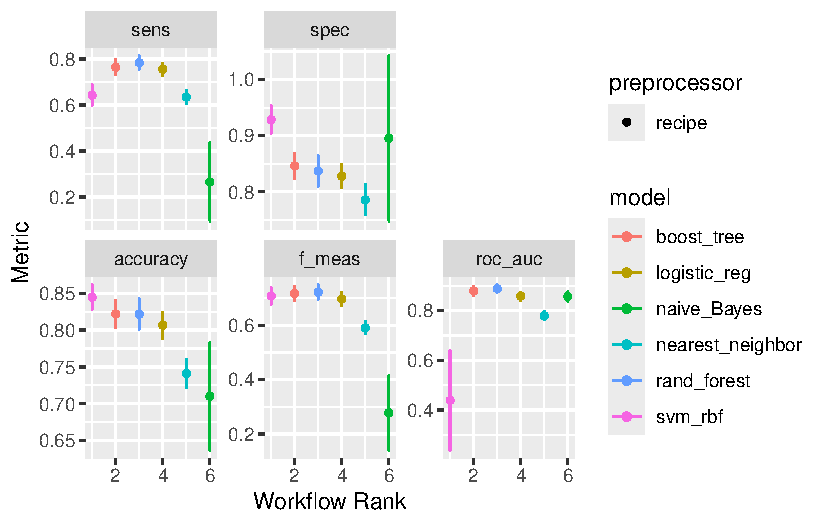
\includegraphics{Quarto_files/figure-pdf/unnamed-chunk-11-1.pdf}

\begin{Shaded}
\begin{Highlighting}[]
\CommentTok{\# {-}{-}{-}{-}{-}{-}{-}{-}{-}{-}{-}{-}{-}{-}{-}{-}{-}{-}{-}{-}{-}{-}{-}{-}{-}{-}{-}{-}{-}{-}{-}{-}{-}{-}{-}{-}{-}{-}{-}{-}{-}{-}{-}{-}{-}{-}{-}{-}{-}{-}{-}{-}{-}{-}{-}{-}{-}{-}{-}{-}{-}{-}{-}{-}{-}{-}{-}{-}{-}{-}{-}{-}{-}{-}{-}{-}{-}{-}}
\CommentTok{\# 9. Plot modeller efter deres performance}
\CommentTok{\# {-}{-}{-}{-}{-}{-}{-}{-}{-}{-}{-}{-}{-}{-}{-}{-}{-}{-}{-}{-}{-}{-}{-}{-}{-}{-}{-}{-}{-}{-}{-}{-}{-}{-}{-}{-}{-}{-}{-}{-}{-}{-}{-}{-}{-}{-}{-}{-}{-}{-}{-}{-}{-}{-}{-}{-}{-}{-}{-}{-}{-}{-}{-}{-}{-}{-}{-}{-}{-}{-}{-}{-}{-}{-}{-}{-}{-}{-}}

\CommentTok{\# Tibble}
\NormalTok{metrics\_df }\OtherTok{\textless{}{-}}\NormalTok{ tibble}\SpecialCharTok{::}\FunctionTok{tibble}\NormalTok{(}
  \AttributeTok{wflow\_id =} \FunctionTok{c}\NormalTok{(}\StringTok{"churn\_recipe\_rf"}\NormalTok{, }\StringTok{"churn\_recipe\_xgboost"}\NormalTok{, }\StringTok{"churn\_recipe\_svm\_rbf"}\NormalTok{,}
               \StringTok{"churn\_recipe\_logistic"}\NormalTok{, }\StringTok{"churn\_recipe\_knn"}\NormalTok{, }\StringTok{"churn\_recipe\_naive\_bayes"}\NormalTok{),}
  \AttributeTok{accuracy =} \FunctionTok{c}\NormalTok{(}\FloatTok{0.825}\NormalTok{, }\FloatTok{0.827}\NormalTok{, }\FloatTok{0.845}\NormalTok{, }\FloatTok{0.807}\NormalTok{, }\FloatTok{0.743}\NormalTok{, }\FloatTok{0.710}\NormalTok{),}
  \AttributeTok{f\_meas   =} \FunctionTok{c}\NormalTok{(}\FloatTok{0.724}\NormalTok{, }\FloatTok{0.723}\NormalTok{, }\FloatTok{0.708}\NormalTok{, }\FloatTok{0.697}\NormalTok{, }\FloatTok{0.592}\NormalTok{, }\FloatTok{0.287}\NormalTok{),}
  \AttributeTok{roc\_auc  =} \FunctionTok{c}\NormalTok{(}\FloatTok{0.877}\NormalTok{, }\FloatTok{0.881}\NormalTok{, }\FloatTok{0.439}\NormalTok{, }\FloatTok{0.858}\NormalTok{, }\FloatTok{0.778}\NormalTok{, }\FloatTok{0.855}\NormalTok{),}
  \AttributeTok{sens     =} \FunctionTok{c}\NormalTok{(}\FloatTok{0.777}\NormalTok{, }\FloatTok{0.766}\NormalTok{, }\FloatTok{0.643}\NormalTok{, }\FloatTok{0.755}\NormalTok{, }\FloatTok{0.634}\NormalTok{, }\FloatTok{0.272}\NormalTok{),}
  \AttributeTok{spec     =} \FunctionTok{c}\NormalTok{(}\FloatTok{0.845}\NormalTok{, }\FloatTok{0.852}\NormalTok{, }\FloatTok{0.929}\NormalTok{, }\FloatTok{0.828}\NormalTok{, }\FloatTok{0.788}\NormalTok{, }\FloatTok{0.893}\NormalTok{)}
\NormalTok{)}

\CommentTok{\# Pivot til langt format}
\NormalTok{metrics\_long }\OtherTok{\textless{}{-}}\NormalTok{ metrics\_df }\SpecialCharTok{\%\textgreater{}\%}
  \FunctionTok{pivot\_longer}\NormalTok{(}\AttributeTok{cols =} \SpecialCharTok{{-}}\NormalTok{wflow\_id, }\AttributeTok{names\_to =} \StringTok{"metric"}\NormalTok{, }\AttributeTok{values\_to =} \StringTok{"score"}\NormalTok{)}

\CommentTok{\# Gør labels pænere}
\NormalTok{metrics\_focus }\OtherTok{\textless{}{-}}\NormalTok{ metrics\_long }\SpecialCharTok{\%\textgreater{}\%}
  \FunctionTok{filter}\NormalTok{(metric }\SpecialCharTok{\%in\%} \FunctionTok{c}\NormalTok{(}\StringTok{"accuracy"}\NormalTok{, }\StringTok{"f\_meas"}\NormalTok{, }\StringTok{"roc\_auc"}\NormalTok{)) }\SpecialCharTok{\%\textgreater{}\%}
  \FunctionTok{mutate}\NormalTok{(}\AttributeTok{metric =} \FunctionTok{case\_when}\NormalTok{(}
\NormalTok{    metric }\SpecialCharTok{==} \StringTok{"accuracy"} \SpecialCharTok{\textasciitilde{}} \StringTok{"Accuracy"}\NormalTok{,}
\NormalTok{    metric }\SpecialCharTok{==} \StringTok{"f\_meas"} \SpecialCharTok{\textasciitilde{}} \StringTok{"F1{-}score"}\NormalTok{,}
\NormalTok{    metric }\SpecialCharTok{==} \StringTok{"roc\_auc"} \SpecialCharTok{\textasciitilde{}} \StringTok{"ROC AUC"}\NormalTok{,}
    \ConstantTok{TRUE} \SpecialCharTok{\textasciitilde{}}\NormalTok{ metric}
\NormalTok{  ))}

\CommentTok{\# 9.1 BarPlot med værdier for denne 3 metrikker}

\FunctionTok{ggplot}\NormalTok{(metrics\_focus, }\FunctionTok{aes}\NormalTok{(}\AttributeTok{x =}\NormalTok{ metric, }\AttributeTok{y =}\NormalTok{ score, }\AttributeTok{fill =}\NormalTok{ metric)) }\SpecialCharTok{+}
  \FunctionTok{geom\_col}\NormalTok{(}\AttributeTok{show.legend =} \ConstantTok{FALSE}\NormalTok{) }\SpecialCharTok{+}
  \FunctionTok{geom\_text}\NormalTok{(}\FunctionTok{aes}\NormalTok{(}\AttributeTok{label =} \FunctionTok{round}\NormalTok{(score, }\DecValTok{2}\NormalTok{)), }\AttributeTok{vjust =} \SpecialCharTok{{-}}\FloatTok{0.3}\NormalTok{, }\AttributeTok{size =} \FloatTok{3.5}\NormalTok{) }\SpecialCharTok{+}
  \FunctionTok{facet\_wrap}\NormalTok{(}\SpecialCharTok{\textasciitilde{}}\NormalTok{ wflow\_id) }\SpecialCharTok{+}
  \FunctionTok{ylim}\NormalTok{(}\DecValTok{0}\NormalTok{, }\FloatTok{1.05}\NormalTok{) }\SpecialCharTok{+}
  \FunctionTok{labs}\NormalTok{(}
    \AttributeTok{title =} \StringTok{"Model performance (Accuracy, F1 og ROC AUC)"}\NormalTok{,}
    \AttributeTok{x =} \ConstantTok{NULL}\NormalTok{,}
    \AttributeTok{y =} \StringTok{"Score"}
\NormalTok{  ) }\SpecialCharTok{+}
  \FunctionTok{theme\_minimal}\NormalTok{() }\SpecialCharTok{+}
  \FunctionTok{theme}\NormalTok{(}
    \AttributeTok{axis.text.x =} \FunctionTok{element\_text}\NormalTok{(}\AttributeTok{angle =} \DecValTok{0}\NormalTok{),}
    \AttributeTok{plot.title =} \FunctionTok{element\_text}\NormalTok{(}\AttributeTok{hjust =} \FloatTok{0.5}\NormalTok{, }\AttributeTok{size =} \DecValTok{14}\NormalTok{, }\AttributeTok{face =} \StringTok{"bold"}\NormalTok{)}
\NormalTok{  ) }\SpecialCharTok{+}
  \FunctionTok{scale\_fill\_brewer}\NormalTok{(}\AttributeTok{palette =} \StringTok{"Set3"}\NormalTok{)}
\end{Highlighting}
\end{Shaded}

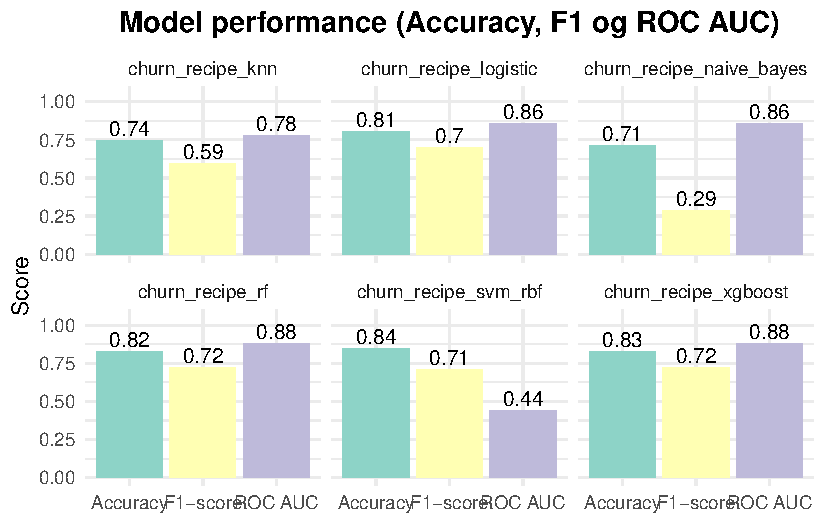
\includegraphics{Quarto_files/figure-pdf/unnamed-chunk-12-1.pdf}

\begin{Shaded}
\begin{Highlighting}[]
\FunctionTok{ggsave}\NormalTok{(}\StringTok{"images/1\_model\_performance.png"}\NormalTok{, }\AttributeTok{width =} \DecValTok{7}\NormalTok{, }\AttributeTok{height =} \DecValTok{4}\NormalTok{, }\AttributeTok{dpi =} \DecValTok{300}\NormalTok{)}


\CommentTok{\# 9.2 Linjeplot}


\FunctionTok{ggplot}\NormalTok{(metrics\_focus, }\FunctionTok{aes}\NormalTok{(}\AttributeTok{x =}\NormalTok{ wflow\_id, }\AttributeTok{y =}\NormalTok{ score, }\AttributeTok{color =}\NormalTok{ metric, }\AttributeTok{group =}\NormalTok{ metric)) }\SpecialCharTok{+}
  \FunctionTok{geom\_line}\NormalTok{(}\AttributeTok{size =} \DecValTok{1}\NormalTok{) }\SpecialCharTok{+}
  \FunctionTok{geom\_point}\NormalTok{(}\AttributeTok{size =} \DecValTok{3}\NormalTok{) }\SpecialCharTok{+}
  \FunctionTok{geom\_text}\NormalTok{(}\FunctionTok{aes}\NormalTok{(}\AttributeTok{label =} \FunctionTok{round}\NormalTok{(score, }\DecValTok{2}\NormalTok{)), }\AttributeTok{vjust =} \SpecialCharTok{{-}}\FloatTok{0.7}\NormalTok{, }\AttributeTok{size =} \DecValTok{3}\NormalTok{) }\SpecialCharTok{+}
  \FunctionTok{scale\_color\_brewer}\NormalTok{(}\AttributeTok{palette =} \StringTok{"Dark2"}\NormalTok{) }\SpecialCharTok{+}
  \FunctionTok{labs}\NormalTok{(}
    \AttributeTok{title =} \StringTok{"Sammenligning på tværs af modeller"}\NormalTok{,}
    \AttributeTok{x =} \StringTok{"Model"}\NormalTok{,}
    \AttributeTok{y =} \StringTok{"Score"}
\NormalTok{  ) }\SpecialCharTok{+}
  \FunctionTok{theme\_minimal}\NormalTok{() }\SpecialCharTok{+}
  \FunctionTok{theme}\NormalTok{(}
    \AttributeTok{axis.text.x =} \FunctionTok{element\_text}\NormalTok{(}\AttributeTok{angle =} \DecValTok{45}\NormalTok{, }\AttributeTok{hjust =} \DecValTok{1}\NormalTok{),}
    \AttributeTok{plot.title =} \FunctionTok{element\_text}\NormalTok{(}\AttributeTok{hjust =} \FloatTok{0.5}\NormalTok{)}
\NormalTok{  )}
\end{Highlighting}
\end{Shaded}

\begin{verbatim}
Warning: Using `size` aesthetic for lines was deprecated in ggplot2 3.4.0.
i Please use `linewidth` instead.
\end{verbatim}

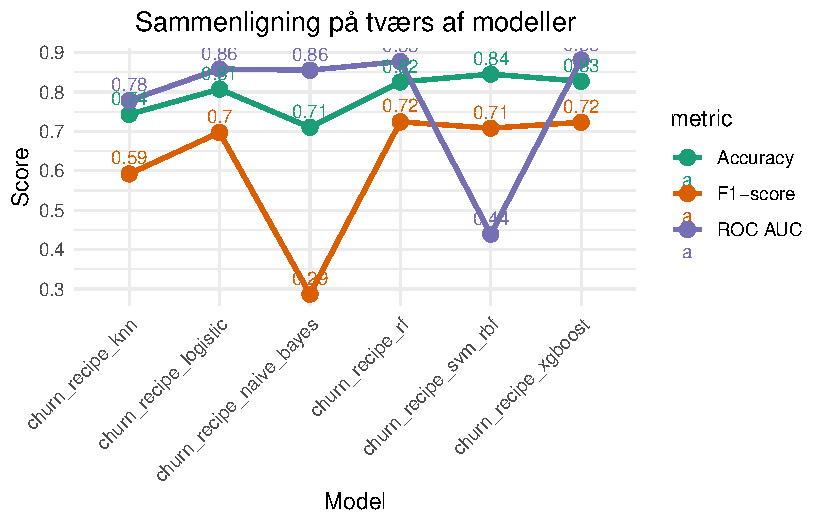
\includegraphics{Quarto_files/figure-pdf/unnamed-chunk-12-2.pdf}

\begin{Shaded}
\begin{Highlighting}[]
\FunctionTok{ggsave}\NormalTok{(}\StringTok{"images/2\_linje\_plot.png"}\NormalTok{, }\AttributeTok{width =} \DecValTok{7}\NormalTok{, }\AttributeTok{height =} \DecValTok{4}\NormalTok{, }\AttributeTok{dpi =} \DecValTok{300}\NormalTok{)}


\CommentTok{\# 9.3 Heatmap pr. model og metrik}


\FunctionTok{ggplot}\NormalTok{(metrics\_focus, }\FunctionTok{aes}\NormalTok{(}\AttributeTok{x =}\NormalTok{ metric, }\AttributeTok{y =}\NormalTok{ wflow\_id, }\AttributeTok{fill =}\NormalTok{ score)) }\SpecialCharTok{+}
  \FunctionTok{geom\_tile}\NormalTok{(}\AttributeTok{color =} \StringTok{"white"}\NormalTok{) }\SpecialCharTok{+}
  \FunctionTok{geom\_text}\NormalTok{(}\FunctionTok{aes}\NormalTok{(}\AttributeTok{label =} \FunctionTok{round}\NormalTok{(score, }\DecValTok{2}\NormalTok{)), }\AttributeTok{size =} \DecValTok{3}\NormalTok{) }\SpecialCharTok{+}
  \FunctionTok{scale\_fill\_gradient}\NormalTok{(}\AttributeTok{low =} \StringTok{"white"}\NormalTok{, }\AttributeTok{high =} \StringTok{"steelblue"}\NormalTok{) }\SpecialCharTok{+}
  \FunctionTok{labs}\NormalTok{(}
    \AttributeTok{title =} \StringTok{"Performance heatmap pr. model og metrik"}\NormalTok{,}
    \AttributeTok{x =} \StringTok{"Metric"}\NormalTok{,}
    \AttributeTok{y =} \StringTok{"Model"}
\NormalTok{  ) }\SpecialCharTok{+}
  \FunctionTok{theme\_minimal}\NormalTok{() }\SpecialCharTok{+}
  \FunctionTok{theme}\NormalTok{(}\AttributeTok{plot.title =} \FunctionTok{element\_text}\NormalTok{(}\AttributeTok{hjust =} \FloatTok{0.5}\NormalTok{))}
\end{Highlighting}
\end{Shaded}

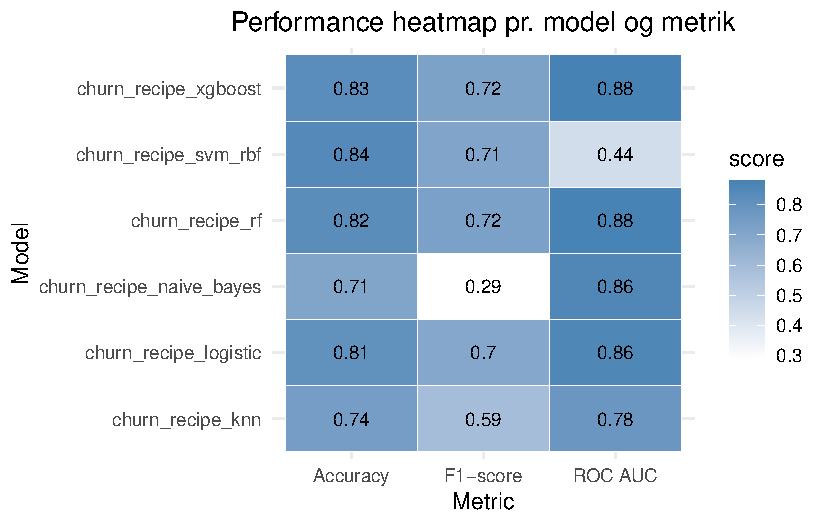
\includegraphics{Quarto_files/figure-pdf/unnamed-chunk-12-3.pdf}

\begin{Shaded}
\begin{Highlighting}[]
\FunctionTok{ggsave}\NormalTok{(}\StringTok{"images/3\_heatmap\_pr\_model.png"}\NormalTok{, }\AttributeTok{width =} \DecValTok{7}\NormalTok{, }\AttributeTok{height =} \DecValTok{4}\NormalTok{, }\AttributeTok{dpi =} \DecValTok{300}\NormalTok{)}


\CommentTok{\# 9.4 Plot for xgboost og Random forest med de vigtigste variabler }


\CommentTok{\# Hent tuning{-}resultater for rf og xgboost}
\NormalTok{rf\_result }\OtherTok{\textless{}{-}}\NormalTok{ churn\_results }\SpecialCharTok{\%\textgreater{}\%} \FunctionTok{extract\_workflow\_set\_result}\NormalTok{(}\StringTok{"churn\_recipe\_rf"}\NormalTok{)}
\NormalTok{xgb\_result }\OtherTok{\textless{}{-}}\NormalTok{ churn\_results }\SpecialCharTok{\%\textgreater{}\%} \FunctionTok{extract\_workflow\_set\_result}\NormalTok{(}\StringTok{"churn\_recipe\_xgboost"}\NormalTok{)}

\CommentTok{\# Hent workflow (før det er fit)}
\NormalTok{rf\_workflow }\OtherTok{\textless{}{-}}\NormalTok{ churn\_results }\SpecialCharTok{\%\textgreater{}\%} \FunctionTok{extract\_workflow}\NormalTok{(}\StringTok{"churn\_recipe\_rf"}\NormalTok{)}
\NormalTok{xgb\_workflow }\OtherTok{\textless{}{-}}\NormalTok{ churn\_results }\SpecialCharTok{\%\textgreater{}\%} \FunctionTok{extract\_workflow}\NormalTok{(}\StringTok{"churn\_recipe\_xgboost"}\NormalTok{)}

\CommentTok{\# Vælg bedste parametre og fit modellen}
\NormalTok{best\_rf }\OtherTok{\textless{}{-}}\NormalTok{ rf\_workflow }\SpecialCharTok{\%\textgreater{}\%}
  \FunctionTok{finalize\_workflow}\NormalTok{(}\FunctionTok{select\_best}\NormalTok{(rf\_result, }\AttributeTok{metric =} \StringTok{"f\_meas"}\NormalTok{)) }\SpecialCharTok{\%\textgreater{}\%}
  \FunctionTok{fit}\NormalTok{(}\AttributeTok{data =}\NormalTok{ churn\_train)}

\NormalTok{best\_xgb }\OtherTok{\textless{}{-}}\NormalTok{ xgb\_workflow }\SpecialCharTok{\%\textgreater{}\%}
  \FunctionTok{finalize\_workflow}\NormalTok{(}\FunctionTok{select\_best}\NormalTok{(xgb\_result, }\AttributeTok{metric =} \StringTok{"f\_meas"}\NormalTok{)) }\SpecialCharTok{\%\textgreater{}\%}
  \FunctionTok{fit}\NormalTok{(}\AttributeTok{data =}\NormalTok{ churn\_train)}

\CommentTok{\# Feature importance}
\NormalTok{vip\_rf }\OtherTok{\textless{}{-}} \FunctionTok{vi}\NormalTok{(}\FunctionTok{extract\_fit\_parsnip}\NormalTok{(best\_rf)) }\SpecialCharTok{\%\textgreater{}\%} \FunctionTok{mutate}\NormalTok{(}\AttributeTok{model =} \StringTok{"Random Forest"}\NormalTok{)}
\NormalTok{vip\_xgb }\OtherTok{\textless{}{-}} \FunctionTok{vi}\NormalTok{(}\FunctionTok{extract\_fit\_parsnip}\NormalTok{(best\_xgb)) }\SpecialCharTok{\%\textgreater{}\%} \FunctionTok{mutate}\NormalTok{(}\AttributeTok{model =} \StringTok{"XGBoost"}\NormalTok{)}

\CommentTok{\# Kombinér og vis kun top 10 vigtigste variabler pr. model}
\NormalTok{vip\_combined }\OtherTok{\textless{}{-}} \FunctionTok{bind\_rows}\NormalTok{(vip\_rf, vip\_xgb) }\SpecialCharTok{\%\textgreater{}\%}
  \FunctionTok{group\_by}\NormalTok{(model) }\SpecialCharTok{\%\textgreater{}\%}
  \FunctionTok{slice\_max}\NormalTok{(}\AttributeTok{order\_by =}\NormalTok{ Importance, }\AttributeTok{n =} \DecValTok{10}\NormalTok{) }\SpecialCharTok{\%\textgreater{}\%}
  \FunctionTok{ungroup}\NormalTok{() }\SpecialCharTok{\%\textgreater{}\%}
  \FunctionTok{mutate}\NormalTok{(}\AttributeTok{Variable =} \FunctionTok{str\_wrap}\NormalTok{(Variable, }\AttributeTok{width =} \DecValTok{25}\NormalTok{))}

\CommentTok{\# Plot med labels og tekstrotation optimeret}
\FunctionTok{ggplot}\NormalTok{(vip\_combined, }\FunctionTok{aes}\NormalTok{(}\AttributeTok{x =} \FunctionTok{reorder}\NormalTok{(Variable, Importance), }\AttributeTok{y =}\NormalTok{ Importance, }\AttributeTok{fill =}\NormalTok{ model)) }\SpecialCharTok{+}
  \FunctionTok{geom\_col}\NormalTok{(}\AttributeTok{show.legend =} \ConstantTok{FALSE}\NormalTok{) }\SpecialCharTok{+}
  \FunctionTok{geom\_text}\NormalTok{(}\FunctionTok{aes}\NormalTok{(}\AttributeTok{label =} \FunctionTok{round}\NormalTok{(Importance, }\DecValTok{2}\NormalTok{)), }\AttributeTok{hjust =} \SpecialCharTok{{-}}\FloatTok{0.1}\NormalTok{, }\AttributeTok{size =} \DecValTok{3}\NormalTok{) }\SpecialCharTok{+}
  \FunctionTok{facet\_wrap}\NormalTok{(}\SpecialCharTok{\textasciitilde{}}\NormalTok{ model, }\AttributeTok{scales =} \StringTok{"free"}\NormalTok{) }\SpecialCharTok{+}
  \FunctionTok{coord\_flip}\NormalTok{() }\SpecialCharTok{+}
  \FunctionTok{labs}\NormalTok{(}
    \AttributeTok{title =} \StringTok{"Top 10 vigtigste variabler pr. model"}\NormalTok{,}
    \AttributeTok{x =} \StringTok{"Variabel"}\NormalTok{,}
    \AttributeTok{y =} \StringTok{"Vigtighed"}
\NormalTok{  ) }\SpecialCharTok{+}
  \FunctionTok{theme\_minimal}\NormalTok{() }\SpecialCharTok{+}
  \FunctionTok{theme}\NormalTok{(}
    \AttributeTok{plot.title =} \FunctionTok{element\_text}\NormalTok{(}\AttributeTok{hjust =} \FloatTok{0.5}\NormalTok{, }\AttributeTok{size =} \DecValTok{14}\NormalTok{, }\AttributeTok{face =} \StringTok{"bold"}\NormalTok{),}
    \AttributeTok{strip.text =} \FunctionTok{element\_text}\NormalTok{(}\AttributeTok{size =} \DecValTok{12}\NormalTok{, }\AttributeTok{face =} \StringTok{"bold"}\NormalTok{),}
    \AttributeTok{axis.text.y =} \FunctionTok{element\_text}\NormalTok{(}\AttributeTok{size =} \DecValTok{9}\NormalTok{)}
\NormalTok{  ) }\SpecialCharTok{+}
  \FunctionTok{scale\_y\_continuous}\NormalTok{(}\AttributeTok{expand =} \FunctionTok{expansion}\NormalTok{(}\AttributeTok{mult =} \FunctionTok{c}\NormalTok{(}\DecValTok{0}\NormalTok{, }\FloatTok{0.10}\NormalTok{))) }\CommentTok{\#ektra space til labels}
\end{Highlighting}
\end{Shaded}

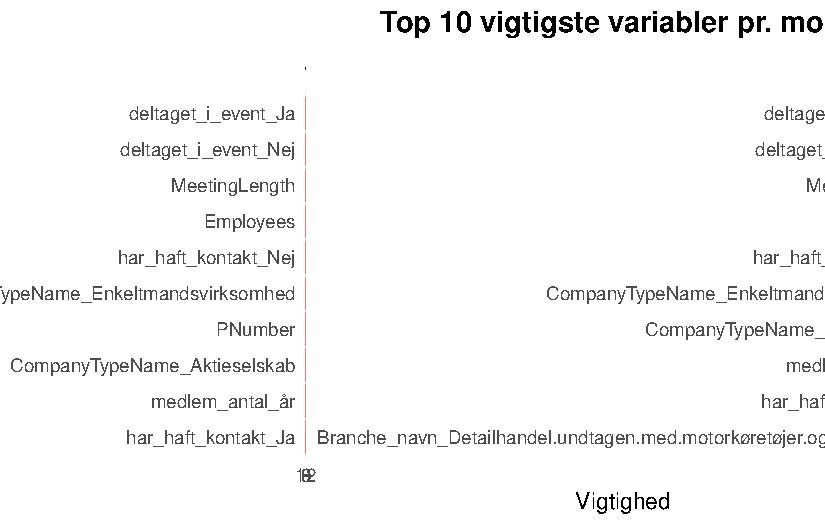
\includegraphics{Quarto_files/figure-pdf/unnamed-chunk-12-4.pdf}

\begin{Shaded}
\begin{Highlighting}[]
\FunctionTok{ggsave}\NormalTok{(}\StringTok{"images/4\_top\_10\_variabler\_pr\_model.png"}\NormalTok{, }\AttributeTok{width =} \DecValTok{7}\NormalTok{, }\AttributeTok{height =} \DecValTok{4}\NormalTok{, }\AttributeTok{dpi =} \DecValTok{300}\NormalTok{)}
\end{Highlighting}
\end{Shaded}

\begin{Shaded}
\begin{Highlighting}[]
\CommentTok{\# {-}{-}{-}{-}{-}{-}{-}{-}{-}{-}{-}{-}{-}{-}{-}{-}{-}{-}{-}{-}{-}{-}{-}{-}{-}{-}{-}{-}{-}{-}{-}{-}{-}{-}{-}{-}{-}{-}{-}{-}{-}{-}{-}{-}{-}{-}{-}{-}{-}{-}{-}{-}{-}{-}{-}{-}{-}{-}{-}{-}{-}{-}{-}{-}{-}{-}{-}{-}{-}{-}{-}{-}{-}{-}{-}{-}{-}{-}}
\CommentTok{\# 10. Endelig model – Finetuning af Random Forest}
\CommentTok{\# {-}{-}{-}{-}{-}{-}{-}{-}{-}{-}{-}{-}{-}{-}{-}{-}{-}{-}{-}{-}{-}{-}{-}{-}{-}{-}{-}{-}{-}{-}{-}{-}{-}{-}{-}{-}{-}{-}{-}{-}{-}{-}{-}{-}{-}{-}{-}{-}{-}{-}{-}{-}{-}{-}{-}{-}{-}{-}{-}{-}{-}{-}{-}{-}{-}{-}{-}{-}{-}{-}{-}{-}{-}{-}{-}{-}{-}{-}}

\CommentTok{\# Undersøg på hele datasæt}

\CommentTok{\# 10.1 Vi laver et workflow med kun én model: Random Forest}
\NormalTok{churn\_workflow\_set\_rf }\OtherTok{\textless{}{-}} \FunctionTok{workflow\_set}\NormalTok{(}
  \AttributeTok{preproc =} \FunctionTok{list}\NormalTok{(}\AttributeTok{churn\_recipe =}\NormalTok{ churn\_recipe),}
  \AttributeTok{models  =} \FunctionTok{list}\NormalTok{(}\AttributeTok{rf =}\NormalTok{ rf\_spec)  }\CommentTok{\# kun én model}
\NormalTok{)}

\CommentTok{\# 10.2 Tænd for parallelisering}
\FunctionTok{plan}\NormalTok{(multisession)}

\CommentTok{\# 10.3 Start tidstagning}
\NormalTok{strt.time }\OtherTok{\textless{}{-}} \FunctionTok{Sys.time}\NormalTok{()}
\end{Highlighting}
\end{Shaded}

\begin{Shaded}
\begin{Highlighting}[]
\CommentTok{\# 10.4 Tuning af kun Random Forest med 25 kombinationer}
\NormalTok{churn\_results\_rf }\OtherTok{\textless{}{-}}\NormalTok{ churn\_workflow\_set\_rf }\SpecialCharTok{|\textgreater{}}
  \FunctionTok{workflow\_map}\NormalTok{(}
    \AttributeTok{resamples =}\NormalTok{ churn\_folds,}
    \AttributeTok{grid =} \DecValTok{25}\NormalTok{,}
    \AttributeTok{metrics =}\NormalTok{ churn\_metrics,}
    \AttributeTok{control =}\NormalTok{ grid\_ctrl,}
    \AttributeTok{seed =} \DecValTok{2025}
\NormalTok{  )}
\end{Highlighting}
\end{Shaded}

\begin{Shaded}
\begin{Highlighting}[]
\CommentTok{\# 10.5 Tid brugt}
\FunctionTok{Sys.time}\NormalTok{() }\SpecialCharTok{{-}}\NormalTok{ strt.time}
\end{Highlighting}
\end{Shaded}

\begin{verbatim}
Time difference of 58.99045 secs
\end{verbatim}

\begin{Shaded}
\begin{Highlighting}[]
\CommentTok{\# 10.6 Sluk for parallelisering}
\FunctionTok{plan}\NormalTok{(sequential)}

\CommentTok{\# 10.7 Vis bedste resultater pr. metrik}
\NormalTok{churn\_results\_rf }\SpecialCharTok{|\textgreater{}} 
  \FunctionTok{rank\_results}\NormalTok{(}\AttributeTok{select\_best =} \ConstantTok{TRUE}\NormalTok{) }\SpecialCharTok{|\textgreater{}} 
  \FunctionTok{select}\NormalTok{(wflow\_id, .metric, mean) }\SpecialCharTok{|\textgreater{}} 
  \FunctionTok{pivot\_wider}\NormalTok{(}\AttributeTok{names\_from =}\NormalTok{ .metric, }\AttributeTok{values\_from =}\NormalTok{ mean) }\SpecialCharTok{|\textgreater{}} 
  \FunctionTok{arrange}\NormalTok{(}\SpecialCharTok{{-}}\NormalTok{f\_meas)}
\end{Highlighting}
\end{Shaded}

\begin{verbatim}
# A tibble: 1 x 6
  wflow_id        accuracy f_meas roc_auc  sens  spec
  <chr>              <dbl>  <dbl>   <dbl> <dbl> <dbl>
1 churn_recipe_rf    0.827  0.728   0.891 0.784 0.845
\end{verbatim}

\begin{Shaded}
\begin{Highlighting}[]
\CommentTok{\# 10.8 Visualisér den bedste model}
\FunctionTok{autoplot}\NormalTok{(churn\_results\_rf, }\AttributeTok{select\_best =} \ConstantTok{TRUE}\NormalTok{)}
\end{Highlighting}
\end{Shaded}

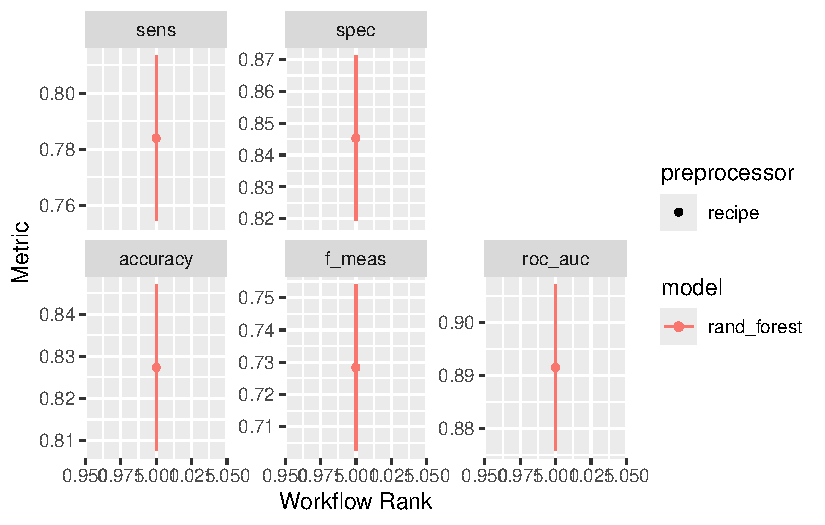
\includegraphics{Quarto_files/figure-pdf/unnamed-chunk-15-1.pdf}

\begin{Shaded}
\begin{Highlighting}[]
\CommentTok{\# {-}{-}{-}{-}{-}{-}{-}{-}{-}{-}{-}{-}{-}{-}{-}{-}{-}{-}{-}{-}{-}{-}{-}{-}{-}{-}{-}{-}{-}{-}{-}{-}{-}{-}{-}{-}{-}{-}{-}{-}{-}{-}{-}{-}{-}{-}{-}{-}{-}{-}{-}{-}{-}{-}{-}{-}{-}{-}{-}{-}{-}{-}{-}{-}{-}{-}{-}{-}{-}{-}{-}{-}{-}{-}{-}{-}{-}{-}}
\CommentTok{\# 11. Evaluering af bedste model på testdatasættet (Random Forest) }
\CommentTok{\# {-}{-}{-}{-}{-}{-}{-}{-}{-}{-}{-}{-}{-}{-}{-}{-}{-}{-}{-}{-}{-}{-}{-}{-}{-}{-}{-}{-}{-}{-}{-}{-}{-}{-}{-}{-}{-}{-}{-}{-}{-}{-}{-}{-}{-}{-}{-}{-}{-}{-}{-}{-}{-}{-}{-}{-}{-}{-}{-}{-}{-}{-}{-}{-}{-}{-}{-}{-}{-}{-}{-}{-}{-}{-}{-}{-}{-}{-}}

\CommentTok{\# Bemærk: Modellen i dette afsnit er baseret på finetuning med 25 kombinationer}

\CommentTok{\# 1. Find bedste parametre for den bedste model}
\NormalTok{best\_results }\OtherTok{\textless{}{-}}\NormalTok{ churn\_results\_rf }\SpecialCharTok{|\textgreater{}}
  \FunctionTok{extract\_workflow\_set\_result}\NormalTok{(}\StringTok{"churn\_recipe\_rf"}\NormalTok{) }\SpecialCharTok{|\textgreater{}}
  \FunctionTok{select\_best}\NormalTok{(}\AttributeTok{metric =} \StringTok{"f\_meas"}\NormalTok{)}

\CommentTok{\# 2. Finaliser workflow med de fundne parametre}
\NormalTok{final\_wf }\OtherTok{\textless{}{-}}\NormalTok{ churn\_results\_rf }\SpecialCharTok{|\textgreater{}}
  \FunctionTok{extract\_workflow}\NormalTok{(}\StringTok{"churn\_recipe\_rf"}\NormalTok{) }\SpecialCharTok{|\textgreater{}}
  \FunctionTok{finalize\_workflow}\NormalTok{(best\_results)}

\CommentTok{\# 3. Træn modellen på træningsdata og evaluer på testdata}
\NormalTok{churn\_last\_fit }\OtherTok{\textless{}{-}}\NormalTok{ final\_wf }\SpecialCharTok{|\textgreater{}} 
  \FunctionTok{last\_fit}\NormalTok{(}\AttributeTok{split =}\NormalTok{ churn\_split, }\AttributeTok{metrics =}\NormalTok{ churn\_metrics)}

\CommentTok{\# 4. Udskriv evalueringsmetrikker}
\FunctionTok{collect\_metrics}\NormalTok{(churn\_last\_fit)}
\end{Highlighting}
\end{Shaded}

\begin{verbatim}
# A tibble: 5 x 4
  .metric  .estimator .estimate .config             
  <chr>    <chr>          <dbl> <chr>               
1 accuracy binary         0.863 Preprocessor1_Model1
2 f_meas   binary         0.789 Preprocessor1_Model1
3 sens     binary         0.868 Preprocessor1_Model1
4 spec     binary         0.861 Preprocessor1_Model1
5 roc_auc  binary         0.931 Preprocessor1_Model1
\end{verbatim}

\begin{Shaded}
\begin{Highlighting}[]
\CommentTok{\# 5. Gem confusion matrix som objekt (brugbar til præsentation)}
\NormalTok{conf\_matrix }\OtherTok{\textless{}{-}}\NormalTok{ churn\_last\_fit }\SpecialCharTok{|\textgreater{}} 
  \FunctionTok{collect\_predictions}\NormalTok{() }\SpecialCharTok{|\textgreater{}} 
  \FunctionTok{conf\_mat}\NormalTok{(}\AttributeTok{estimate =}\NormalTok{ .pred\_class, }\AttributeTok{truth =}\NormalTok{ churn)}

\CommentTok{\# 6. Gem test{-}prædiktioner hvis ønsket}
\NormalTok{test\_preds }\OtherTok{\textless{}{-}} \FunctionTok{collect\_predictions}\NormalTok{(churn\_last\_fit)}

\CommentTok{\# 7. Træn endelig model på hele datasættet}
\NormalTok{final\_model }\OtherTok{\textless{}{-}} \FunctionTok{fit}\NormalTok{(final\_wf, }\AttributeTok{data =}\NormalTok{ feature\_engineering)}

\CommentTok{\# 8. Gem modellen}
\FunctionTok{saveRDS}\NormalTok{(final\_model, }\StringTok{"final\_churn\_model.rds"}\NormalTok{)}


\CommentTok{\# 11.1 Eksempel: Forudsig churn for én ny virksomhed}


\NormalTok{new\_company }\OtherTok{\textless{}{-}} \FunctionTok{tibble}\NormalTok{(}
  \AttributeTok{Employees =} \DecValTok{15}\NormalTok{,}
  \AttributeTok{PostalCode =} \FunctionTok{factor}\NormalTok{(}\StringTok{"8800"}\NormalTok{),}
  \AttributeTok{CompanyTypeName =} \FunctionTok{factor}\NormalTok{(}\StringTok{"Aktieselskab"}\NormalTok{),}
  \AttributeTok{har\_haft\_kontakt =} \FunctionTok{factor}\NormalTok{(}\StringTok{"Ja"}\NormalTok{),}
  \AttributeTok{deltaget\_i\_event =} \FunctionTok{factor}\NormalTok{(}\StringTok{"Nej"}\NormalTok{),}
\NormalTok{  hjælp}\AttributeTok{\_kategori =} \FunctionTok{factor}\NormalTok{(}\StringTok{"Strategi Udvikling"}\NormalTok{),}
\NormalTok{  medlem\_antal\_å}\AttributeTok{r =} \DecValTok{2}\NormalTok{,}
  \AttributeTok{Branche\_navn =} \FunctionTok{factor}\NormalTok{(}\StringTok{"Fremstilling af maskiner og udstyr i.a.n."}\NormalTok{),}
  \AttributeTok{MeetingLength =} \DecValTok{180}\NormalTok{,}
  \AttributeTok{PNumber =} \DecValTok{12345678}
\NormalTok{)}

\CommentTok{\# Forudsiger klassifikation og sandsynlighed}
\FunctionTok{predict}\NormalTok{(final\_model, new\_company)                    }\CommentTok{\# 0 = bliver, 1 = churn}
\end{Highlighting}
\end{Shaded}

\begin{verbatim}
# A tibble: 1 x 1
  .pred_class
  <fct>      
1 0          
\end{verbatim}

\begin{Shaded}
\begin{Highlighting}[]
\FunctionTok{predict}\NormalTok{(final\_model, new\_company, }\AttributeTok{type =} \StringTok{"prob"}\NormalTok{)     }\CommentTok{\# churn{-}sandsynlighed}
\end{Highlighting}
\end{Shaded}

\begin{verbatim}
# A tibble: 1 x 2
  .pred_0 .pred_1
    <dbl>   <dbl>
1   0.668   0.332
\end{verbatim}

\begin{Shaded}
\begin{Highlighting}[]
\CommentTok{\# 11.2 Forudsig churn for ALLE virksomheder og tilføj resultater}


\CommentTok{\# Modellen anvendes nu på hele medlemsdatabasen for at identificere churn{-}risiko}

\CommentTok{\# Forudsiger sandsynlighed og klasse}
\NormalTok{churn\_probs   }\OtherTok{\textless{}{-}} \FunctionTok{predict}\NormalTok{(final\_model, feature\_engineering, }\AttributeTok{type =} \StringTok{"prob"}\NormalTok{)}
\NormalTok{churn\_classes }\OtherTok{\textless{}{-}} \FunctionTok{predict}\NormalTok{(final\_model, feature\_engineering)}

\CommentTok{\# Kombiner og omdøb kolonner}
\NormalTok{all\_predictions }\OtherTok{\textless{}{-}} \FunctionTok{bind\_cols}\NormalTok{(churn\_probs, churn\_classes) }\SpecialCharTok{|\textgreater{}} 
  \FunctionTok{rename}\NormalTok{(}
    \AttributeTok{churn\_prob =}\NormalTok{ .pred\_1,      }\CommentTok{\# Sandsynlighed for churn}
    \AttributeTok{churn\_class =}\NormalTok{ .pred\_class  }\CommentTok{\# Klassifikation (0/1)}
\NormalTok{  )}

\CommentTok{\# Tilføj til datasættet og konvertér sandsynlighed til procent}
\NormalTok{full\_results }\OtherTok{\textless{}{-}}\NormalTok{ feature\_engineering }\SpecialCharTok{|\textgreater{}} 
  \FunctionTok{bind\_cols}\NormalTok{(all\_predictions) }\SpecialCharTok{|\textgreater{}} 
  \FunctionTok{mutate}\NormalTok{(}
    \AttributeTok{churn\_prob =} \FunctionTok{round}\NormalTok{(churn\_prob }\SpecialCharTok{*} \DecValTok{100}\NormalTok{, }\DecValTok{1}\NormalTok{)}
\NormalTok{  ) }

\CommentTok{\# Tilføj churn{-}risikokategorier tidligt (bruges i visualiseringer og rapporter)}
\NormalTok{full\_results }\OtherTok{\textless{}{-}}\NormalTok{ full\_results }\SpecialCharTok{|\textgreater{}} 
  \FunctionTok{mutate}\NormalTok{(}
    \AttributeTok{churn\_risiko =} \FunctionTok{case\_when}\NormalTok{(}
\NormalTok{      churn\_prob }\SpecialCharTok{\textgreater{}=} \DecValTok{80} \SpecialCharTok{\textasciitilde{}} \StringTok{"Høj risiko"}\NormalTok{,}
\NormalTok{      churn\_prob }\SpecialCharTok{\textgreater{}=} \DecValTok{60} \SpecialCharTok{\textasciitilde{}} \StringTok{"Moderat risiko"}\NormalTok{,}
\NormalTok{      churn\_prob }\SpecialCharTok{\textgreater{}=} \DecValTok{40} \SpecialCharTok{\textasciitilde{}} \StringTok{"Lav risiko"}\NormalTok{,}
      \ConstantTok{TRUE}             \SpecialCharTok{\textasciitilde{}} \StringTok{"Minimal risiko"}
\NormalTok{    )}
\NormalTok{  )}


\CommentTok{\# 11.3 Visualisering: Fordeling af churn{-}risikokategorier (kun aktive medlemmer)}


\NormalTok{full\_results }\SpecialCharTok{|\textgreater{}} 
  \FunctionTok{filter}\NormalTok{(churn }\SpecialCharTok{==} \DecValTok{0}\NormalTok{) }\SpecialCharTok{|\textgreater{}}  
  \FunctionTok{count}\NormalTok{(churn\_risiko) }\SpecialCharTok{|\textgreater{}} 
  \FunctionTok{ggplot}\NormalTok{(}\FunctionTok{aes}\NormalTok{(}\AttributeTok{x =} \FunctionTok{reorder}\NormalTok{(churn\_risiko, }\SpecialCharTok{{-}}\NormalTok{n), }\AttributeTok{y =}\NormalTok{ n, }\AttributeTok{fill =}\NormalTok{ churn\_risiko)) }\SpecialCharTok{+}
  \FunctionTok{geom\_col}\NormalTok{(}\AttributeTok{show.legend =} \ConstantTok{FALSE}\NormalTok{) }\SpecialCharTok{+}
  \FunctionTok{geom\_text}\NormalTok{(}\FunctionTok{aes}\NormalTok{(}\AttributeTok{label =}\NormalTok{ n), }\AttributeTok{vjust =} \SpecialCharTok{{-}}\DecValTok{1}\NormalTok{, }\AttributeTok{size =} \DecValTok{5}\NormalTok{) }\SpecialCharTok{+}
  \FunctionTok{scale\_fill\_manual}\NormalTok{(}\AttributeTok{values =} \FunctionTok{c}\NormalTok{(}
    \StringTok{"Minimal risiko"} \OtherTok{=} \StringTok{"darkgreen"}\NormalTok{,}
    \StringTok{"Lav risiko"}     \OtherTok{=} \StringTok{"green4"}\NormalTok{,}
    \StringTok{"Moderat risiko"} \OtherTok{=} \StringTok{"orange"}\NormalTok{,}
    \StringTok{"Høj risiko"}     \OtherTok{=} \StringTok{"darkred"}
\NormalTok{  )) }\SpecialCharTok{+}
  \FunctionTok{scale\_y\_continuous}\NormalTok{(}\AttributeTok{expand =} \FunctionTok{expansion}\NormalTok{(}\AttributeTok{mult =} \FunctionTok{c}\NormalTok{(}\DecValTok{0}\NormalTok{, }\FloatTok{0.1}\NormalTok{))) }\SpecialCharTok{+}  
  \FunctionTok{coord\_cartesian}\NormalTok{(}\AttributeTok{clip =} \StringTok{"off"}\NormalTok{) }\SpecialCharTok{+}
  \FunctionTok{labs}\NormalTok{(}
    \AttributeTok{title =} \StringTok{"Fordeling af churn{-}risiko blandt aktive medlemmer"}\NormalTok{,}
    \AttributeTok{subtitle =} \StringTok{"Kategorier: Minimal (\textless{}40\%), Lav (40–59.9\%), Moderat (60–79.9\%), Høj (80–100\%)"}\NormalTok{,}
    \AttributeTok{x =} \StringTok{"Risikokategori"}\NormalTok{,}
    \AttributeTok{y =} \StringTok{"Antal virksomheder"}
\NormalTok{  ) }\SpecialCharTok{+}
  \FunctionTok{theme\_minimal}\NormalTok{()}
\end{Highlighting}
\end{Shaded}

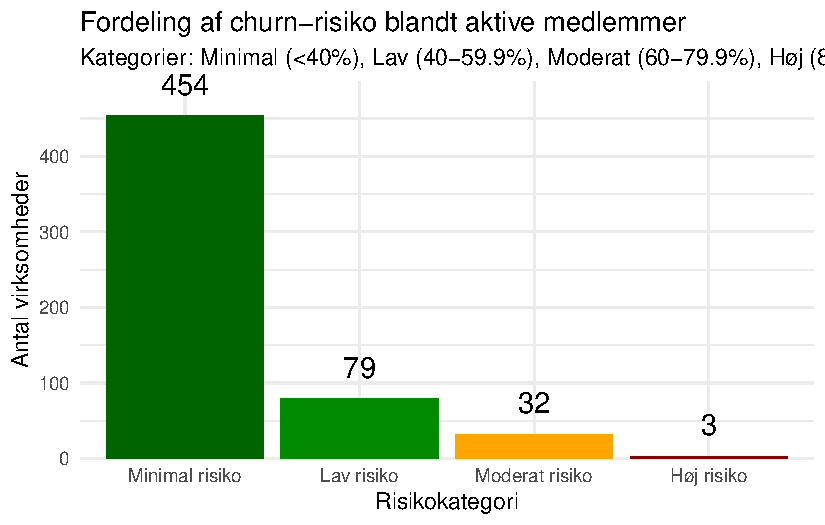
\includegraphics{Quarto_files/figure-pdf/unnamed-chunk-16-1.pdf}

\begin{Shaded}
\begin{Highlighting}[]
\FunctionTok{ggsave}\NormalTok{(}\StringTok{"images/9\_churn\_risikokategorier\_aktive.png"}\NormalTok{, }\AttributeTok{width =} \DecValTok{7}\NormalTok{, }\AttributeTok{height =} \DecValTok{4}\NormalTok{, }\AttributeTok{dpi =} \DecValTok{300}\NormalTok{)}

\CommentTok{\# 11.4 Churn{-}risiko: Filtrér medlemmer (churn == 0) med høj risiko (churn\_class == 1)}


\NormalTok{top\_risiko\_medlemmer }\OtherTok{\textless{}{-}}\NormalTok{ full\_results }\SpecialCharTok{|\textgreater{}} 
  \FunctionTok{filter}\NormalTok{(churn }\SpecialCharTok{==} \DecValTok{0}\NormalTok{, churn\_class }\SpecialCharTok{==} \DecValTok{1}\NormalTok{) }\SpecialCharTok{|\textgreater{}} 
  \FunctionTok{arrange}\NormalTok{(}\FunctionTok{desc}\NormalTok{(churn\_prob)) }\SpecialCharTok{|\textgreater{}} 
  \FunctionTok{slice\_head}\NormalTok{(}\AttributeTok{n =} \DecValTok{20}\NormalTok{)  }\CommentTok{\# Call to action: top 20}


\CommentTok{\# 11.5 Visualiseringer: Brancher og postnumre med høj churn}


\CommentTok{\# Brancher med højest gennemsnitlig churn}
\NormalTok{full\_results }\SpecialCharTok{|\textgreater{}} 
  \FunctionTok{group\_by}\NormalTok{(Branche\_navn) }\SpecialCharTok{|\textgreater{}} 
  \FunctionTok{summarise}\NormalTok{(}\AttributeTok{gennemsnitlig\_churn =} \FunctionTok{mean}\NormalTok{(churn\_prob), }\AttributeTok{n =} \FunctionTok{n}\NormalTok{()) }\SpecialCharTok{|\textgreater{}} 
  \FunctionTok{arrange}\NormalTok{(}\FunctionTok{desc}\NormalTok{(gennemsnitlig\_churn)) }\SpecialCharTok{|\textgreater{}} 
  \FunctionTok{slice\_head}\NormalTok{(}\AttributeTok{n =} \DecValTok{5}\NormalTok{) }\SpecialCharTok{|\textgreater{}} 
  \FunctionTok{ggplot}\NormalTok{(}\FunctionTok{aes}\NormalTok{(}\AttributeTok{x =} \FunctionTok{reorder}\NormalTok{(Branche\_navn, gennemsnitlig\_churn), }\AttributeTok{y =}\NormalTok{ gennemsnitlig\_churn)) }\SpecialCharTok{+}
  \FunctionTok{geom\_col}\NormalTok{(}\AttributeTok{fill =} \StringTok{"steelblue"}\NormalTok{) }\SpecialCharTok{+}
  \FunctionTok{coord\_flip}\NormalTok{() }\SpecialCharTok{+}
  \FunctionTok{labs}\NormalTok{(}\AttributeTok{title =} \StringTok{"Top 5 churn{-}risiko"}\NormalTok{, }\AttributeTok{x =} \StringTok{"Branche"}\NormalTok{, }\AttributeTok{y =} \StringTok{"Gns. churn sandsynlighed (\%)"}\NormalTok{) }\SpecialCharTok{+}
  \FunctionTok{theme\_minimal}\NormalTok{()}
\end{Highlighting}
\end{Shaded}

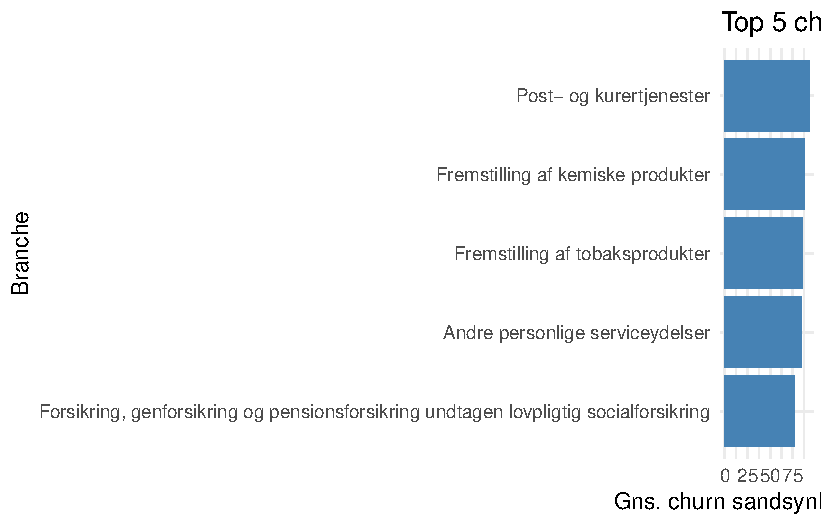
\includegraphics{Quarto_files/figure-pdf/unnamed-chunk-16-2.pdf}

\begin{Shaded}
\begin{Highlighting}[]
\FunctionTok{ggsave}\NormalTok{(}\StringTok{"images/5\_brancher\_højeste\_churn.png"}\NormalTok{, }\AttributeTok{width =} \DecValTok{7}\NormalTok{, }\AttributeTok{height =} \DecValTok{4}\NormalTok{, }\AttributeTok{dpi =} \DecValTok{300}\NormalTok{)}

\CommentTok{\# Postnumre med højest gennemsnitlig churn}
\NormalTok{full\_results }\SpecialCharTok{|\textgreater{}} 
  \FunctionTok{group\_by}\NormalTok{(PostalCode) }\SpecialCharTok{|\textgreater{}} 
  \FunctionTok{summarise}\NormalTok{(}\AttributeTok{gennemsnitlig\_churn =} \FunctionTok{mean}\NormalTok{(churn\_prob), }\AttributeTok{n =} \FunctionTok{n}\NormalTok{()) }\SpecialCharTok{|\textgreater{}} 
  \FunctionTok{arrange}\NormalTok{(}\FunctionTok{desc}\NormalTok{(gennemsnitlig\_churn)) }\SpecialCharTok{|\textgreater{}} 
  \FunctionTok{slice\_head}\NormalTok{(}\AttributeTok{n =} \DecValTok{5}\NormalTok{) }\SpecialCharTok{|\textgreater{}} 
  \FunctionTok{ggplot}\NormalTok{(}\FunctionTok{aes}\NormalTok{(}\AttributeTok{x =} \FunctionTok{reorder}\NormalTok{(}\FunctionTok{as.character}\NormalTok{(PostalCode), gennemsnitlig\_churn), }\AttributeTok{y =}\NormalTok{ gennemsnitlig\_churn)) }\SpecialCharTok{+}
  \FunctionTok{geom\_col}\NormalTok{(}\AttributeTok{fill =} \StringTok{"darkred"}\NormalTok{) }\SpecialCharTok{+}
  \FunctionTok{coord\_flip}\NormalTok{() }\SpecialCharTok{+}
  \FunctionTok{labs}\NormalTok{(}\AttributeTok{title =} \StringTok{"Top 5 postnumre med højest churn{-}risiko"}\NormalTok{, }\AttributeTok{x =} \StringTok{"Postnummer"}\NormalTok{, }\AttributeTok{y =} \StringTok{"Gns. churn sandsynlighed (\%)"}\NormalTok{) }\SpecialCharTok{+}
  \FunctionTok{theme\_minimal}\NormalTok{()}
\end{Highlighting}
\end{Shaded}

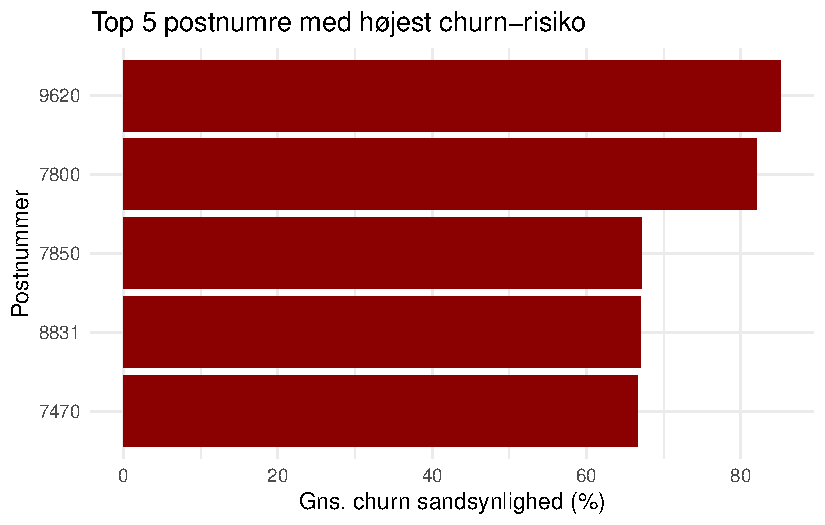
\includegraphics{Quarto_files/figure-pdf/unnamed-chunk-16-3.pdf}

\begin{Shaded}
\begin{Highlighting}[]
\FunctionTok{ggsave}\NormalTok{(}\StringTok{"images/6\_postnummer\_højeste\_churn.png"}\NormalTok{, }\AttributeTok{width =} \DecValTok{7}\NormalTok{, }\AttributeTok{height =} \DecValTok{4}\NormalTok{, }\AttributeTok{dpi =} \DecValTok{300}\NormalTok{)}

\CommentTok{\# 11.6 Hvad kendetegner virksomheder der IKKE churner?}

\NormalTok{full\_results }\SpecialCharTok{|\textgreater{}} 
  \FunctionTok{filter}\NormalTok{(churn\_class }\SpecialCharTok{==} \DecValTok{0}\NormalTok{) }\SpecialCharTok{|\textgreater{}}  \CommentTok{\# Virksomheder som modellen forudser bliver}
  \FunctionTok{count}\NormalTok{(Branche\_navn, }\AttributeTok{sort =} \ConstantTok{TRUE}\NormalTok{) }\SpecialCharTok{|\textgreater{}} 
  \FunctionTok{slice\_head}\NormalTok{(}\AttributeTok{n =} \DecValTok{5}\NormalTok{) }\SpecialCharTok{|\textgreater{}} 
  \FunctionTok{ggplot}\NormalTok{(}\FunctionTok{aes}\NormalTok{(}\AttributeTok{x =} \FunctionTok{reorder}\NormalTok{(Branche\_navn, n), }\AttributeTok{y =}\NormalTok{ n)) }\SpecialCharTok{+}
  \FunctionTok{geom\_col}\NormalTok{(}\AttributeTok{fill =} \StringTok{"forestgreen"}\NormalTok{) }\SpecialCharTok{+}
  \FunctionTok{coord\_flip}\NormalTok{() }\SpecialCharTok{+}
  \FunctionTok{labs}\NormalTok{(}
    \AttributeTok{title =} \StringTok{"Top 5 der ikke churner"}\NormalTok{,}
    \AttributeTok{x =} \StringTok{"Branche"}\NormalTok{,}
    \AttributeTok{y =} \StringTok{"Antal virksomheder"}
\NormalTok{  ) }\SpecialCharTok{+}
  \FunctionTok{theme\_minimal}\NormalTok{()}
\end{Highlighting}
\end{Shaded}

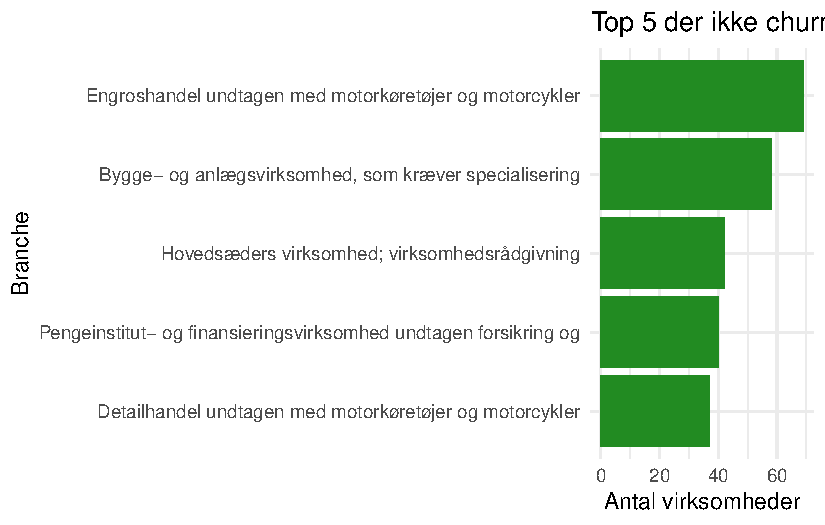
\includegraphics{Quarto_files/figure-pdf/unnamed-chunk-16-4.pdf}

\begin{Shaded}
\begin{Highlighting}[]
\FunctionTok{ggsave}\NormalTok{(}\StringTok{"images/7\_top5\_der\_ikke\_churner.png"}\NormalTok{, }\AttributeTok{width =} \DecValTok{7}\NormalTok{, }\AttributeTok{height =} \DecValTok{4}\NormalTok{, }\AttributeTok{dpi =} \DecValTok{300}\NormalTok{)}

\CommentTok{\# Sammenlignende statistik på udvalgte variabler}
\CommentTok{\# churn\_class:}
\CommentTok{\# 0 = modellen tror de bliver}
\CommentTok{\# 1 = modellen tror de churner}
\NormalTok{full\_results }\SpecialCharTok{|\textgreater{}} 
  \FunctionTok{group\_by}\NormalTok{(churn\_class) }\SpecialCharTok{|\textgreater{}} 
  \FunctionTok{summarise}\NormalTok{(}
\NormalTok{    mødelængde }\OtherTok{=} \FunctionTok{mean}\NormalTok{(MeetingLength),}
\NormalTok{    medlem\_å}\AttributeTok{r =} \FunctionTok{mean}\NormalTok{(medlem\_antal\_år),}
    \AttributeTok{kontakt\_rate =} \FunctionTok{mean}\NormalTok{(har\_haft\_kontakt }\SpecialCharTok{==} \StringTok{"Ja"}\NormalTok{),}
    \AttributeTok{event\_rate =} \FunctionTok{mean}\NormalTok{(deltaget\_i\_event }\SpecialCharTok{==} \StringTok{"Ja"}\NormalTok{)}
\NormalTok{  )}
\end{Highlighting}
\end{Shaded}

\begin{verbatim}
# A tibble: 2 x 5
  churn_class mødelængde medlem_år kontakt_rate event_rate
  <fct>            <dbl>     <dbl>        <dbl>      <dbl>
1 0                30.5       8.23        0.568     0.829 
2 1                 3.50      7.73        0.232     0.0210
\end{verbatim}

\begin{Shaded}
\begin{Highlighting}[]
\CommentTok{\# 11.7 Hvad er de vigtigste variabler}

\CommentTok{\# 1. Udtræk tuning{-}resultater og workflow}
\NormalTok{rf\_result }\OtherTok{\textless{}{-}}\NormalTok{ churn\_results\_rf }\SpecialCharTok{|\textgreater{}} \FunctionTok{extract\_workflow\_set\_result}\NormalTok{(}\StringTok{"churn\_recipe\_rf"}\NormalTok{)}
\NormalTok{rf\_workflow }\OtherTok{\textless{}{-}}\NormalTok{ churn\_results\_rf }\SpecialCharTok{|\textgreater{}} \FunctionTok{extract\_workflow}\NormalTok{(}\StringTok{"churn\_recipe\_rf"}\NormalTok{)}

\CommentTok{\# 2. Find bedste parametre og træn modellen på træningsdata}
\NormalTok{best\_rf }\OtherTok{\textless{}{-}}\NormalTok{ rf\_workflow }\SpecialCharTok{|\textgreater{}}
  \FunctionTok{finalize\_workflow}\NormalTok{(}\FunctionTok{select\_best}\NormalTok{(rf\_result, }\AttributeTok{metric =} \StringTok{"f\_meas"}\NormalTok{)) }\SpecialCharTok{|\textgreater{}}
  \FunctionTok{fit}\NormalTok{(}\AttributeTok{data =}\NormalTok{ churn\_train)}

\CommentTok{\# 3. Brug vip til at finde top 10 vigtigste variabler}
\NormalTok{vip\_rf }\OtherTok{\textless{}{-}} \FunctionTok{vi}\NormalTok{(}\FunctionTok{extract\_fit\_parsnip}\NormalTok{(best\_rf)) }\SpecialCharTok{|\textgreater{}}
  \FunctionTok{slice\_max}\NormalTok{(}\AttributeTok{order\_by =}\NormalTok{ Importance, }\AttributeTok{n =} \DecValTok{5}\NormalTok{) }\SpecialCharTok{|\textgreater{}}
  \FunctionTok{mutate}\NormalTok{(}\AttributeTok{Variable =} \FunctionTok{str\_wrap}\NormalTok{(Variable, }\AttributeTok{width =} \DecValTok{30}\NormalTok{))}

\CommentTok{\# 4. Plot}
\FunctionTok{ggplot}\NormalTok{(vip\_rf, }\FunctionTok{aes}\NormalTok{(}\AttributeTok{x =} \FunctionTok{reorder}\NormalTok{(Variable, Importance), }\AttributeTok{y =}\NormalTok{ Importance)) }\SpecialCharTok{+}
  \FunctionTok{geom\_col}\NormalTok{(}\AttributeTok{fill =} \StringTok{"steelblue"}\NormalTok{) }\SpecialCharTok{+}
  \FunctionTok{coord\_flip}\NormalTok{() }\SpecialCharTok{+}
  \FunctionTok{labs}\NormalTok{(}
    \AttributeTok{title =} \StringTok{"Top 5 variabler (RF)"}\NormalTok{,}
    \AttributeTok{x =} \StringTok{"Variabel"}\NormalTok{,}
    \AttributeTok{y =} \StringTok{"Vigtighed"}
\NormalTok{  ) }\SpecialCharTok{+}
  \FunctionTok{theme\_minimal}\NormalTok{() }\SpecialCharTok{+}
  \FunctionTok{theme}\NormalTok{(}
    \AttributeTok{plot.title =} \FunctionTok{element\_text}\NormalTok{(}\AttributeTok{hjust =} \FloatTok{0.5}\NormalTok{, }\AttributeTok{size =} \DecValTok{14}\NormalTok{, }\AttributeTok{face =} \StringTok{"bold"}\NormalTok{),}
    \AttributeTok{axis.text.y =} \FunctionTok{element\_text}\NormalTok{(}\AttributeTok{size =} \DecValTok{10}\NormalTok{)}
\NormalTok{  )}
\end{Highlighting}
\end{Shaded}

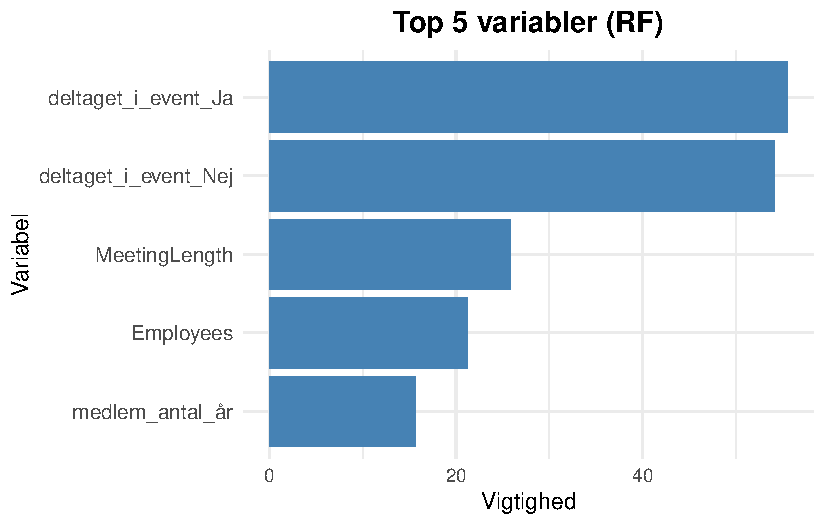
\includegraphics{Quarto_files/figure-pdf/unnamed-chunk-16-5.pdf}

\begin{Shaded}
\begin{Highlighting}[]
\CommentTok{\# 5. Gem billedet}
\FunctionTok{ggsave}\NormalTok{(}\StringTok{"images/8\_top\_5\_variabler\_rf.png"}\NormalTok{, }\AttributeTok{width =} \DecValTok{7}\NormalTok{, }\AttributeTok{height =} \DecValTok{4}\NormalTok{, }\AttributeTok{dpi =} \DecValTok{300}\NormalTok{)}

\CommentTok{\# Gemmer full\_results som RDS}
\FunctionTok{saveRDS}\NormalTok{(full\_results, }\StringTok{"full\_results.rds"}\NormalTok{)}
\end{Highlighting}
\end{Shaded}

\begin{Shaded}
\begin{Highlighting}[]
\CommentTok{\# {-}{-}{-}{-}{-}{-}{-}{-}{-}{-}{-}{-}{-}{-}{-}{-}{-}{-}{-}{-}{-}{-}{-}{-}{-}{-}{-}{-}{-}{-}{-}{-}{-}{-}{-}{-}{-}{-}{-}{-}{-}{-}{-}{-}{-}{-}{-}{-}{-}{-}{-}{-}{-}{-}{-}{-}{-}{-}{-}{-}{-}{-}{-}{-}{-}{-}{-}{-}{-}{-}{-}{-}{-}{-}{-}{-}{-}{-}}
\CommentTok{\# 12 Churn dashboard til Business Viborg}
\CommentTok{\# {-}{-}{-}{-}{-}{-}{-}{-}{-}{-}{-}{-}{-}{-}{-}{-}{-}{-}{-}{-}{-}{-}{-}{-}{-}{-}{-}{-}{-}{-}{-}{-}{-}{-}{-}{-}{-}{-}{-}{-}{-}{-}{-}{-}{-}{-}{-}{-}{-}{-}{-}{-}{-}{-}{-}{-}{-}{-}{-}{-}{-}{-}{-}{-}{-}{-}{-}{-}{-}{-}{-}{-}{-}{-}{-}{-}{-}{-}}
\end{Highlighting}
\end{Shaded}





\end{document}
